\documentclass[11pt,a4paper]{article}
\usepackage[margin=25mm]{geometry}
\usepackage[T1]{fontenc}
\usepackage{lmodern}
\usepackage{amsmath,amssymb,amsthm}
\usepackage{booktabs,tabularx,array}
\usepackage{microtype}
\usepackage{xcolor}
\usepackage{tikz}
\usepackage{graphicx}
\usetikzlibrary{arrows.meta,positioning}
\usepackage{pgfplots}
\usepgfplotslibrary{groupplots}
\usepackage[section]{placeins}
\pgfplotsset{compat=1.18}
\usepackage[hidelinks]{hyperref}
\newcommand{\E}{\mathbb{E}}
\newcommand{\R}{\mathbb{R}}
\newcommand{\BA}{\mathrm{BA}}
\newcommand{\MSE}{\mathrm{MSE}}
\newcommand{\NMSE}{\mathrm{NMSE}}
\newcommand{\BCE}{\mathrm{BCE}}
\newcommand{\pp}{\text{ percentage points}}
\newtheorem{proposition}{Proposition}
\renewcommand{\arraystretch}{1.15}
\setlength{\emergencystretch}{2em}
\title{Cross-Channel Prediction, Classification, and Individual Retention in Low-Channel EEG Adaptation}
\author{Yiming Shen$^{1,*}$ \quad Xi Jiang$^{2}$\\[0.6em]
\small $^{1}$University of Massachusetts Boston\\
\small $^{2}$University of Chicago\\
\small $^{*}$Corresponding author: Yiming Shen}
\date{}

\begin{document}
\maketitle

\begin{abstract}
Reliable low-channel electroencephalography (EEG) adaptation requires models to benefit from new information while retaining their earlier performance. When task labels and paired recordings from a larger montage are available, the practical question is which prediction functions improve after updating. We evaluated cross-channel prediction, downstream classification, and individual retention using matched information budgets, fixed feedback-release rules, and initial tests permanently excluded from fitting. In the 42-participant Lee group held out from protocol development, paired calibration reduced omitted-channel feature error relative to frozen mapping. Correct pairing also improved fixed-classifier performance relative to within-class shuffled pairing, but a classification gain over frozen mapping remained unconfirmed. In the 62-participant Stieger development cohort, reduced-label updating improved mean future balanced accuracy by 2.48 percentage points over zero new labels, using 75.3\% fewer new labels than the all-label condition. However, 19 participants scored lower on the permanent initial test than their own initialized model, despite positive future gains against the zero-label control. Separate personal-update experiments evaluated two training-risk constraints; both met future-performance tolerance, but neither confirmed the required reduction in severe old-test declines. Together, these comparisons distinguish gains in calibration accuracy, downstream classification, and retained individual performance. Evaluations of EEG adaptation should connect each information source to the function it improves and report individual retention alongside mean future performance.
\end{abstract}

\noindent\textbf{Keywords:} EEG; low-channel decoding; continual adaptation; paired calibration; cross-channel prediction; individual retention.

\section{Introduction}

Low-channel EEG adaptation aims to improve prediction as additional observations and supervision become available. Task labels inform the decision rule, whereas paired recordings from a larger montage inform the relationship between low- and high-channel measurements. Two evaluation questions follow: whether an improvement in cross-channel prediction reaches the downstream task, and whether participants retain their earlier performance after updating. Calibration accuracy, downstream classification, and performance on initial data therefore require separate evaluation. We examine these questions in systems initialized with a larger montage and subsequently operated with fewer electrodes or less supervision.

Existing EEG adaptation methods address changes between calibration and subsequent use. Unsupervised LDA adaptation targets non-class-related nonstationarity \cite{vidaurre2011}, while reviews of EEG classification distinguish adaptive classifiers, transfer learning, and covariance-based methods \cite{lotte2018}. Transfer learning reuses information across participants or recording sessions \cite{jayaram2016}. Covariance-based classification \cite{barachant2012}, covariance recentering \cite{zanini2018}, and Riemannian Procrustes alignment \cite{rodrigues2019} provide complementary approaches to EEG representation and adaptation.

Three established lines of research inform this evaluation. Learning using privileged information formalizes the use of training information that is unavailable at prediction time \cite{vapnik2009}; generalized distillation connects this setting to teacher--student transfer through softened teacher predictions \cite{lopezpaz2016}. Continual-learning methods protect earlier performance through different update rules: elastic weight consolidation penalizes changes to parameters important for earlier tasks \cite{kirkpatrick2017}, Learning without Forgetting penalizes changes to earlier-task outputs on new-task inputs \cite{li2018}, and Gradient Episodic Memory constrains updates using stored past-task examples \cite{lopezpaz2017}. For EEG evaluation, the Mother of All BCI Benchmarks supports reproducible comparisons across datasets and evaluation settings \cite{jayaram2018}. Together, these approaches address the information available for training, the constraints imposed by earlier examples, and the comparison of predictive performance. We connect these questions through explicit information-release rules, matched controls, and retention tests on initial data permanently excluded from fitting.

Cross-view EEG prediction makes the distinction between calibration and task performance explicit. The keyhole study reported relationships between ear and scalp EEG that depend on electrode location and reference configuration \cite{mikkelsen2017}. A predicted high-channel target estimates a specified representation, and its usefulness for another function requires separate evaluation. Longitudinal neural decoding also draws on different information sources: language-corrected pseudo-labels support decoder recalibration \cite{fan2023}, whereas alignment with learned latent dynamics uses temporal structure \cite{karpowicz2025}. These studies motivate comparisons that identify both the information entering an update and the function subsequently evaluated.

Two EEG studies directly address reconstruction and continual retention. Ramakrishnan and Satyanarayana reconstructed omitted signals and their spectral content using learned inter-channel correlation \cite{ramakrishnan2016}. Duan et al.\ used balanced, informative memory replay to retain EEG decoding performance as participants arrive sequentially \cite{duan2024}. Here, Lee's ERP task tests the downstream value of predicted channels using a fixed classifier, while Stieger tracks initial-test retention within the same participants across sessions. True-pair and class-preserving shuffled updates receive equal calibration budgets; frozen mappings provide the no-new-pair reference. Permanent initial tests reveal individual score changes alongside mean future gains.

The principal analyses use two public EEG datasets with distinct evidence roles. Repeated sessions in Stieger support development and retention analyses \cite{stieger2021}. Lee provides 12 development participants and a separate 42-participant group evaluated under fixed ERP protocols \cite{lee2019}. The extended analyses examine Yang's fixed downstream paired-calibration test \cite{yang2025} and Farabbi's fixed feedback-source direction test \cite{farabbi2020}. Their complete methods, outcomes, and subsequent development diagnostics are reported in Appendix~\ref{app:eeg}.

These controls yield three empirical findings. First, in Lee's 42-participant group held out from protocol development, true pairs improved cross-channel prediction and fixed-classifier performance relative to class-preserving shuffled pairs, while a classification gain over frozen mapping remained unconfirmed. Second, reduced-label updating in the Stieger development cohort improved mean future classification over zero new labels, alongside old-test declines for some participants relative to their own initialized models. Third, matched personal-update experiments showed that line and full-space training-risk constraints met future tolerance but did not confirm the reduction in old-test harm required by the joint criterion. Together, the findings connect information budgets and comparison baselines to downstream benefit and individual retention.

\section{Problem formulation}
\label{sec:problem}

For participant $i$, session $s$, and trial $j$, let $X^L_{isj}$ denote the available low-channel measurement and $X^H_{isj}$ the simultaneously recorded larger montage. The task label is $Y_{isj}$, and $Z^H_{isj}=g_H(X^H_{isj})$ denotes the high-channel prediction target. In the REVE experiments, $Z^H$ comprises fixed, whitened principal-component coordinates of a frozen encoder. In the ERP experiment, it comprises binned amplitudes from the channels omitted from the low view. Both targets are therefore fixed representations derived from the recorded measurements.

The task model $f_\theta$ predicts $Y$ from the low view, while a separate or coupled mapping $m_\phi$ predicts $Z^H$. We evaluate their performance and the change in earlier task performance through distinct endpoints:
\begin{align}
 R_{\mathrm{task}}(\theta)&=\E\{\ell(Y,f_\theta(X^L))\},\\
 R_{\mathrm{view}}(\phi)&=\E\{\|Z^H-m_\phi(X^L)\|^2/d_H\},\\
 \Delta R_{\mathrm{old}}&=R_{\mathrm{old}}(\theta_s)-R_{\mathrm{old}}(\theta_0).
\end{align}
We summarize task performance by balanced accuracy and, where specified, the area under the receiver operating characteristic curve (AUC) \cite{delong1988}. Cross-view prediction is evaluated by mean squared error (MSE), normalized MSE, and skill relative to each participant's actual initial-mean predictor. To assess retention, we compare each updated model with its own initialization on a permanently excluded initial test. Participant-specific changes complement the future and old-test means, which do not identify losses for an individual participant.

In Lee, MSE is computed in fixed ERP coordinates standardized using initial data. Appendix~\ref{app:eeg} gives the distinct definitions of NMSE and mean-predictor skill used in the extended REVE mapping analyses.

\subsection{Information and prediction time}

At prediction time, models can use initial fitting data, previously released feedback and calibration pairs, and observations available up to that time. In Stieger, Yang, and Farabbi, we save predictions from all compared methods before releasing current-session feedback. Shared models apply this rule across participants: every participant in a relative session round is predicted before feedback from any participant in that round is released. These rounds define the analysis schedule, without requiring participants to attend on the same calendar day. In Lee, the designated calibration block becomes available after it ends, and the separately scored test run follows later in the same second session.

Under this schedule, we compare no update, label-only update, pair-only update, and their combination. Pair-only updating receives low inputs and their high targets but does not use their new task labels in the classification objective. The class-preserving shuffle keeps the same new-label and pairing budgets while disrupting exact same-trial alignment. Constructing this control requires class membership, so it serves as a diagnostic comparison rather than a label-free deployment method.

\begin{figure}[t]
\centering
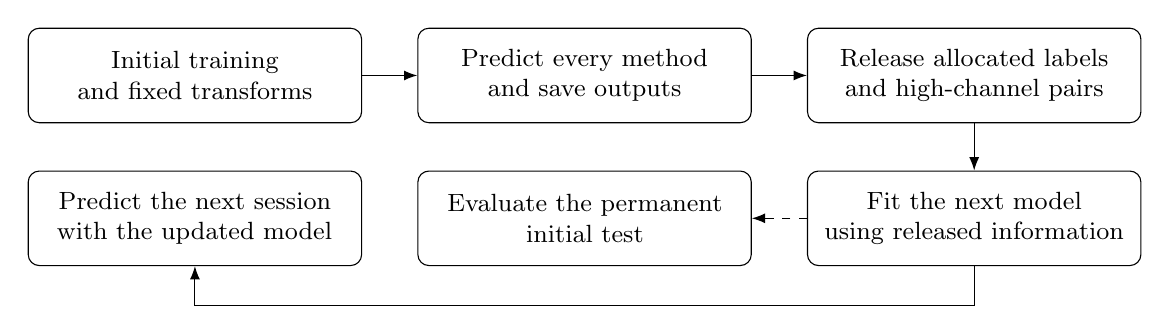
\begin{tikzpicture}[font=\small,node distance=6mm and 7mm,box/.style={draw,rounded corners,align=center,text width=40mm,minimum height=12mm},>=Latex]
\node[box] (init) {Initial training\\and fixed transforms};
\node[box,right=of init] (pred) {Predict every method\\and save outputs};
\node[box,right=of pred] (release) {Release allocated labels\\and high-channel pairs};
\node[box,below=of release] (update) {Fit the next model\\using released information};
\node[box,left=of update] (old) {Evaluate the permanent\\initial test};
\node[box,left=of old] (next) {Predict the next session\\with the updated model};
\draw[->] (init)--(pred);
\draw[->] (pred)--(release);
\draw[->] (release)--(update);
\draw[->] (update.south)--++(0,-5mm)-|(next.south);
\draw[->,dashed] (update)--(old);
\end{tikzpicture}
\caption{Information-release protocol for the session-based EEG comparisons. Predictions are saved before current-session outcomes enter a model. The permanent initial test is excluded from fitting, replay, and normalization, and its scores are excluded from model selection within each frozen stage. Shared models enforce the prediction barrier across participants in each relative session round. In Lee, the completed calibration block precedes the separate future test run.}
\label{fig:timing}
\end{figure}

\section{Materials and methods}

\subsection{Datasets, splits, and evidence roles}

Table~\ref{tab:data} summarizes the primary and extended datasets, which we analyze separately. Stieger provides development data, with the 41-participant longer-follow-up cohort nested in the 62-participant cohort. Lee's original-event comparisons use a separate 42-participant group under a fixed protocol. Yang and Farabbi retain their original fixed-test roles; their subsequent diagnostics are reported as development analyses in Appendix~\ref{app:eeg}.

\begin{table}[tbp]
\centering
\caption{Primary and extended public EEG datasets and their evaluation designs.}
\label{tab:data}
\begingroup
\small
\setlength{\tabcolsep}{5pt}
\renewcommand{\arraystretch}{1.18}
\begin{tabularx}{\linewidth}{@{}
  >{\raggedright\arraybackslash}p{.13\linewidth}
  >{\raggedright\arraybackslash}p{.22\linewidth}
  >{\raggedright\arraybackslash}p{.22\linewidth}
  >{\raggedright\arraybackslash}X@{}}
\toprule
\textbf{Dataset} & \textbf{Participants and follow-up} & \textbf{Measurement views} & \textbf{Evaluation design}\\
\midrule
\textbf{Stieger} &
62 participants\newline
7 sessions\newline
41 participants (nested)\newline
11 sessions &
Low: C3/C4\newline
High: 60 channels &
Primary development analyses: feedback budgets, paired targets, and retention. Successive sessions are predicted before feedback release.\\
\addlinespace[7pt]
\textbf{Lee ERP} &
Development: 12\newline
Confirmation: 42\newline
2 sessions &
Low: Cz/Pz\newline
High: 62 channels &
Primary fixed confirmation protocols. Session 2 training-run calibration precedes its separate test run. Original-event and common-history analyses are separate.\\
\addlinespace[7pt]
\textbf{Yang} &
51 participants\newline
3 sessions &
Low: C3/C4\newline
High: 59 channels &
Extended fixed downstream pairing test. Session 2 feedback precedes the session 3 future test.\\
\addlinespace[7pt]
\textbf{Farabbi} &
12 participants\newline
3 consecutive days &
Low: C3/C4\newline
High: not evaluated &
Extended source-direction confirmation; exploratory constraints. Day 2 updating precedes the day 3 future test.\\
\bottomrule
\end{tabularx}
\par\smallskip
\begin{minipage}{\linewidth}
\footnotesize\raggedright
The high view is the specified larger recorded montage. Farabbi recorded 32 EEG channels; only the C3/C4 view is evaluated here.
\end{minipage}
\endgroup
\end{table}

\paragraph{Stieger.}
The original Stieger dataset contains 62 participants with up to 11 sessions \cite{stieger2021}. We use the left--right task for the 62 participants available through session 7 and the nested 41 available through session 11. The high view comprises the 60 supported scalp channels after removing CB1 and CB2; the low view comprises C3 and C4. We order retained session 1 trials by their original index and divide them into 60\% initial training, 20\% initial development, and 20\% permanent old test, excluding one retained trial immediately before each boundary. The development portion supports the predefined early choice of structure-loss weight and ridge penalty. Later eligibility analyses use the same portion as the fixed initial diagnostic set. This set remains excluded from model fitting, and later stages do not repeat parameter selection on it. Permanent old-test trials are excluded from fitting and normalization. Within each frozen stage, old-test and future scores are excluded from model selection. Earlier result summaries informed subsequent development questions, which retain their development designation.

Initial transforms use the fixed 900-example PhysioNet motor-imagery source from the original experiment. We fit low-view target normalization on initial training data. High-view coordinates use the frozen source normalization and 16-component whitening transform, so the target coordinates remain fixed as new observations arrive. The source data provide common prior training information and do not count as newly acquired target feedback.

\paragraph{Lee ERP.}
The OpenBMI dataset contains two recording sessions from 54 participants \cite{lee2019}. Participants 1--12 form the development group, and participants 13--54 form the 42-participant confirmation group. We fit the initial models on the 33 complete characters in the session 1 training run and reserve the 36 complete characters in its test run as the permanent old test. Calibration uses the first 11 complete characters of the session 2 training run, corresponding to 660 flashes before the history restriction; the remaining training characters are excluded. We then evaluate the fixed models on the 36-character session 2 test run.

The low view comprises Cz/Pz, and the full reference comprises 62 EEG channels with the recorded nasion reference. We filter each run causally with a fourth-order channelwise Butterworth filter from 0.5 to 20\,Hz, starting from a zero filter state. Each epoch uses a $-0.2$ to 0\,s baseline and a 0 to 0.8\,s response window, summarized by sixteen 50\,ms means per channel. Predictions are made 0.8\,s after each flash. Responses to later flashes can overlap this window, so the endpoint is flash-event discrimination rather than character-selection accuracy. Initial means and population standard deviations remain fixed across subsequent models. This experiment uses ERP features without a REVE encoder.

The original-event comparisons include all events permitted by their fixed protocol. Appendix~\ref{sec:history} specifies the separate history-compatible event set, timing features, and history-confirmation comparisons. Those analyses retain their own event masks and interval levels, separate from the principal mapping and classification results.

\subsection{Feature extraction and prediction models}

For Stieger, we use the frozen REVE-base encoder to obtain a 512-dimensional representation by averaging channel and temporal tokens \cite{reve2025}. Low- and high-view representations are extracted independently from their permitted channel sets, without fine-tuning the encoder. Cue-locked windows cover 0--3\,s. We resample from 1,000 to 200\,Hz, then apply fourth-order channelwise 0.5--95\,Hz zero-phase filtering within each window. Within-window population standardization and clipping to $[-15,15]$ preserve the recorded reference. Low-view processing uses only the observed channels, and each prediction uses the complete epoch. Appendix~\ref{app:eeg} describes processing for the extended datasets.

In the separate-head experiments, the task classifier and ridge cross-view mapping are updated independently. Changing a ridge target therefore leaves the separate classifier unchanged. Mapping controls comprise an initial-mean predictor, frozen mapping, output-bias update, correct new pairs, class-centroid targets, and within-class shuffled targets. Comparing true pairs with shuffled targets evaluates the information contributed by exact correspondence beyond task-class grouping for the specified mapping and target.

We initialize direct classifiers using class-balanced initial-training cross-entropy plus $0.001\|w\|^2/2$. After feedback is released, the pooled initial-training loss and cumulative released-feedback loss each receive weight 0.5. The regularizer remains unchanged, and the intercept is unpenalized. The Stieger budget experiment uses shared classifiers. The constraint stages use personal classifiers with global initial-data replay and recipient-specific feedback, with risk constraints evaluated on each recipient's own initial-training trials. Each frozen protocol has its own matched reference models.

For Lee, we fit individual classifiers using linear discriminant analysis, a standard single-trial ERP readout \cite{blankertz2011}, with oracle-approximating shrinkage covariances \cite{chen2010} estimated separately for each class and equal class priors. The current low input contains 32 binned features, and the full input contains 992. An affine ridge mapping with a free intercept and penalty 0.1 predicts the sixteen-bin features of the 60 omitted channels, giving a 960-dimensional target. To evaluate downstream transfer, we apply the classifier trained on the true full view to mapped features while keeping its coefficients fixed. The input combines the observed Cz/Pz features with predictions for the omitted channels. This comparison evaluates the mapping's use by that classifier separately from waveform-feature MSE.

\subsection{Feedback budgets and matched information}

The Stieger budget experiment combines 0\%, approximately 25\%, and 100\% new low-view labels with either no new pairs or three allocations of 40 pairs per participant. The early, uniform, and late allocations each release two batches of 20 pairs. Labels and pairs are selected using fixed, separate orderings, and paired recordings supply no additional task-label budget. No update is performed after the final scored session. Initial training information continues to be replayed with fixed group-loss weights, so accumulating more observations in a group does not increase its loss weight.

Class-preserving shuffled-pair controls retain the pair count and task-class grouping while disrupting exact same-trial correspondence. We evaluate Lee's fixed classifier using each resulting mapping. Appendix~\ref{sec:source} presents the recipient-matched feedback-source comparisons and their complete results.

\subsection{Retention constraints and initial eligibility}

The personal-update stages compare an unconstrained candidate with an update restricted to the line from the initialized model to that candidate and an update optimized over the full coefficient space. Both constrained conditions allow an increase of at most 0.01 in initial-training binary cross-entropy. The line update takes the largest feasible step; the full-space update minimizes the new objective subject to the constraint. Each stage uses its own matched unconstrained reference. Constraints are evaluated on fitting data, with the permanent old test kept separate. Appendix~\ref{sec:retention-extended} reports the complete replay, penalty, optimization, and training-only generalization controls.

Initial task eligibility in Stieger requires balanced accuracy of at least 0.60 on the fixed diagnostic split. Initial target eligibility requires MSE below the participant's initial-mean predictor. The score-change analysis includes all participants, with eligibility categories reported separately. Appendix~\ref{sec:retention-extended} specifies the extended joint-adequacy and repeated-failure rules.

We assess permanent-test harm relative to each model's initial prediction. Severe old-task harm is a decline of at least five balanced-accuracy percentage points. The predefined dual criterion requires the lower 95\% bound of the future-accuracy difference relative to unconstrained personal updating to be at least $-0.5$ percentage points and the upper 95\% bound of the difference in severe-harm proportion to be strictly below zero. Both requirements must hold; meeting the future criterion alone does not meet the dual criterion. These Stieger retention comparisons are development analyses, evaluated using predefined operational thresholds and exploratory intervals.

\subsection{Statistical analysis}

We first compute participant-specific endpoints. For Stieger, we average repeated sessions within each participant before taking the equal-participant mean. The principal comparisons use 10,000 paired participant-bootstrap resamples \cite{efron1979}. Each resample draws participants with replacement and retains their records across the compared methods. Two-sided empirical percentiles give the interval endpoints. Models remain fixed during resampling, so the intervals are conditional on the realized training procedure and exclude variability from refitting shared models or reselecting donors.

Principal contrasts use 95\% intervals. Lee's original-event comparisons use unadjusted, descriptive 95\% intervals within the fixed 42-participant protocol. The extended source comparisons in Stieger 62 and Farabbi, and the Lee ordered-history comparisons, each retain their original family of two main contrasts with Bonferroni-adjusted 97.5\% intervals. Source comparisons in the nested Stieger 41 cohort remain descriptive at 95\%. We retain the comparison families defined by the original stage protocols, without retrospectively adjusting across all development stages. The accompanying statistical-methods record documents stage-specific seeds, resampling counts, comparison families, and recorded software versions. The earliest archived EEG stage used 5,000 resamples, as detailed in Appendix~\ref{app:eeg}. A nonsignificant difference is not interpreted as noninferiority.

\subsection{Evaluation specification}
\label{sec:evaluation-specification}

Table~\ref{tab:evaluation-specification} lists the information required to reproduce an adaptation comparison. We specify these fields before interpreting a gain. The complete evidence index in Appendix~\ref{app:eeg}, Table~\ref{tab:contrasts}, also identifies the role of each extended comparison.

\begin{table}[tbp]
\centering\small
\caption{Minimum specification for evaluating the contribution of an information source and retention of earlier performance. Task labels and paired measurements are counted separately.}
\label{tab:evaluation-specification}
\begin{tabularx}{\linewidth}{@{}>{\raggedright\arraybackslash}p{.20\linewidth}>{\raggedright\arraybackslash}X>{\raggedright\arraybackslash}X@{}}
\toprule
Field & Record before evaluation & Check in the comparison\\
\midrule
Target and function & Task output, specified high-view target, or initial function & Report each function on its own metric and fixed target coordinates.\\
\addlinespace
Information and budget & Task labels, same-trial pairs, and their matched controls & Match the proposed source against a control with the stated information count.\\
\addlinespace
Prediction time & Input window, feedback release, and shared-model barrier & Save predictions before current outcomes or calibration targets become available.\\
\addlinespace
Initial competence & Fixed training identities and, where specified, diagnostic identities and an adequacy rule & Record absent diagnostics or eligibility rules explicitly; report qualification separately and retain all participants.\\
\addlinespace
Retention & Permanent initial test excluded from fitting and, within each frozen stage, model selection & Pair each updated score with its own initialization and show individual changes.\\
\addlinespace
Decision and evidence role & Required contrast, operational threshold, interval, and development or confirmation role & Preserve the original decision; label subsequent diagnostics and numerical checks separately.\\
\bottomrule
\end{tabularx}
\end{table}


\section{Results}

The principal results address three questions: whether paired-calibration gains improve downstream classification, how future classification gains relate to individual old-test changes, and whether training-risk constraints meet the joint retention criterion. The extended controls are reported in Appendix~\ref{app:eeg}.

\subsection{Paired-calibration gains and downstream classification}
\label{sec:mapped-task}

In the fixed 42-participant Lee evaluation, we compared improvements in the calibration target with downstream classification. On the original-event future test, direct low-channel label updating increased AUC from 0.66051 to 0.69001, a difference of 0.02950 ($[0.01821,0.04357]$). Correct paired calibration reduced omitted-channel feature MSE from 1.10264 to 0.90873, with a difference of $-0.19391$ ($[-0.51127,-0.02478]$) relative to frozen mapping. The difference relative to the mean class-preserving shuffle was $-0.35745$ ($[-0.73245,-0.12356]$).

For downstream evaluation, the fixed full-view classifier received observed Cz/Pz and predicted omitted-channel features. Updated mapping yielded an AUC difference of $-0.00220$ relative to frozen mapping (95\% interval $[-0.00968,+0.00402]$), leaving a gain over the existing mapping unconfirmed. Correct pairing improved AUC relative to the mean class-preserving shuffle by $+0.01427$ ($[+0.00547,+0.02298]$). Thus, exact correspondence benefited this classifier compared with disrupted pairing, while lower feature error did not establish a classification gain over frozen mapping. Figure~\ref{fig:eeg-lee-endpoints} reports the original-event controls and individual paired outcomes. The separate 12-participant component diagnostics are reported in Appendix~\ref{sec:lee-diagnostics}.

The participant-level changes varied in direction and magnitude. Relative to frozen mapping, MSE decreased for 40 of 42 participants and mapped AUC increased for 30; eleven participants had lower MSE without higher AUC. These counts describe the directions of observed individual changes. Participant 24 accounted for 78.73\% of the total net MSE reduction, calculated as that participant's reduction divided by the sum across all 42 participants, with MSE increases contributing negatively. All participants remain in the original means and intervals.

% FIGURE_BEGIN:eeg-lee-primary-contrasts
\begin{figure}[p]
\centering
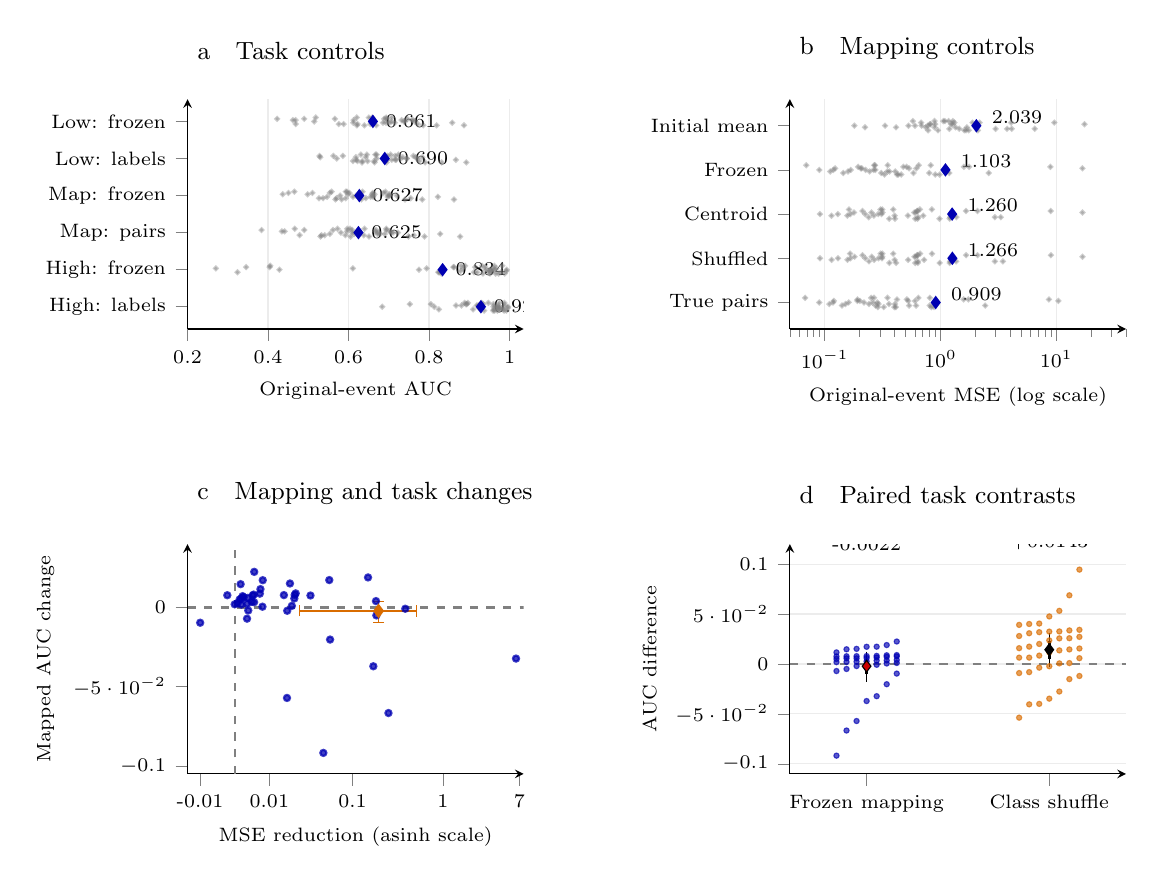
\begin{tikzpicture}
\begin{axis}[axis lines=left,tick align=outside,tick label style={font=\scriptsize},label style={font=\scriptsize},title style={font=\small,align=left},grid style={gray!15},every axis plot/.append style={line width=.8pt},enlarge x limits=false,at={(0cm,0cm)},anchor=north west,width=5.85cm,height=4.5cm,title={a\quad Task controls},title style={font=\small,align=left,at={(0,1.06)},anchor=south west},xlabel={Original-event AUC},xmin=.2,xmax=1.035,ymin=-.6,ymax=5.6,ytick={5,4,3,2,1,0},yticklabels={Low: frozen,Low: labels,Map: frozen,Map: pairs,High: frozen,High: labels},xmajorgrids=true]
\addplot[gray,only marks,mark=*,mark size=.65pt,opacity=.4] coordinates {(0.668723765432,4.895) (0.622220679012,4.93) (0.71500154321,4.965) (0.737311728395,5) (0.612604938272,5.035) (0.688425925926,5.07) (0.650436728395,5.105) (0.639442901235,4.895) (0.575901234568,4.93) (0.701672839506,4.965) (0.664,5) (0.75749382716,5.035) (0.694487654321,5.07) (0.659026234568,5.105) (0.818913580247,4.895) (0.771817901235,4.93) (0.68562345679,4.965) (0.740226851852,5) (0.760220679012,5.035) (0.746029320988,5.07) (0.620472222222,5.105) (0.620699074074,4.895) (0.587854938272,4.93) (0.857538580247,4.965) (0.70649845679,5) (0.468351851852,5.035) (0.489858024691,5.07) (0.518557098765,5.105) (0.88687345679,4.895) (0.654154320988,4.93) (0.693064814815,4.965) (0.764091049383,5) (0.731941358025,5.035) (0.566094135802,5.07) (0.707086419753,5.105) (0.785600308642,4.895) (0.468845679012,4.93) (0.611802469136,4.965) (0.514762345679,5) (0.461695987654,5.035) (0.422709876543,5.07) (0.693398148148,5.105)};
\addplot[gray,only marks,mark=*,mark size=.65pt,opacity=.4] coordinates {(0.694353395062,3.895) (0.647433641975,3.93) (0.715907407407,3.965) (0.744739197531,4) (0.618132716049,4.035) (0.696375,4.07) (0.669717592593,4.105) (0.664580246914,3.895) (0.622172839506,3.93) (0.718591049383,3.965) (0.669820987654,4) (0.783287037037,4.035) (0.715901234568,4.07) (0.66662808642,4.105) (0.831344135802,3.895) (0.775344135802,3.93) (0.696154320988,3.965) (0.744344135802,4) (0.767075617284,4.035) (0.76112345679,4.07) (0.645453703704,4.105) (0.633430555556,3.895) (0.611067901235,3.93) (0.866677469136,3.965) (0.729413580247,4) (0.52962191358,4.035) (0.527808641975,4.07) (0.630804012346,4.105) (0.892481481481,3.895) (0.663427469136,3.93) (0.707385802469,3.965) (0.77074845679,4) (0.734856481481,4.035) (0.585970679012,4.07) (0.723739197531,4.105) (0.790356481481,3.895) (0.634603395062,3.93) (0.619316358025,3.965) (0.570950617284,4) (0.642527777778,4.035) (0.562507716049,4.07) (0.704447530864,4.105)};
\addplot[gray,only marks,mark=*,mark size=.65pt,opacity=.4] coordinates {(0.631925925926,2.895) (0.593,2.93) (0.697101851852,2.965) (0.701970679012,3) (0.598483024691,3.035) (0.602617283951,3.07) (0.558012345679,3.105) (0.582691358025,2.895) (0.526569444444,2.93) (0.661212962963,2.965) (0.618814814815,3) (0.658601851852,3.035) (0.66024845679,3.07) (0.634782407407,3.105) (0.783114197531,2.895) (0.754572530864,2.93) (0.546591049383,2.965) (0.719828703704,3) (0.701942901235,3.035) (0.686938271605,3.07) (0.596091049383,3.105) (0.567399691358,2.895) (0.536649691358,2.93) (0.822035493827,2.965) (0.661114197531,3) (0.436341049383,3.035) (0.510228395062,3.07) (0.465429012346,3.105) (0.862097222222,2.895) (0.642896604938,2.93) (0.654820987654,2.965) (0.698549382716,3) (0.664271604938,3.035) (0.553581790123,3.07) (0.691708333333,3.105) (0.740200617284,2.895) (0.570233024691,2.93) (0.611049382716,2.965) (0.578969135802,3) (0.498337962963,3.035) (0.450584876543,3.07) (0.593336419753,3.105)};
\addplot[gray,only marks,mark=*,mark size=.65pt,opacity=.4] coordinates {(0.65087654321,1.895) (0.592195987654,1.93) (0.690046296296,1.965) (0.710695987654,2) (0.596404320988,2.035) (0.609098765432,2.07) (0.572734567901,2.105) (0.605171296296,1.895) (0.532591049383,1.93) (0.678509259259,1.965) (0.609194444444,2) (0.626365740741,2.035) (0.668171296296,2.07) (0.639824074074,2.105) (0.788787037037,1.895) (0.762134259259,1.93) (0.553722222222,1.965) (0.722523148148,2) (0.702429012346,2.035) (0.69450617284,2.07) (0.603901234568,2.105) (0.530302469136,1.895) (0.540677469136,1.93) (0.827706790123,1.965) (0.672699074074,2) (0.434430555556,2.035) (0.489978395062,2.07) (0.466438271605,2.105) (0.877231481481,1.895) (0.637912037037,1.93) (0.672032407407,1.965) (0.706652777778,2) (0.66662037037,2.035) (0.561313271605,2.07) (0.693550925926,2.105) (0.749101851852,1.895) (0.478475308642,1.93) (0.61462345679,1.965) (0.580984567901,2) (0.44125308642,2.035) (0.383984567901,2.07) (0.596682098765,2.105)};
\addplot[gray,only marks,mark=*,mark size=.65pt,opacity=.4] coordinates {(0.972686728395,0.895) (0.822666666667,0.93) (0.95100617284,0.965) (0.955202160494,1) (0.79412191358,1.035) (0.860532407407,1.07) (0.962240740741,1.105) (0.95149845679,0.895) (0.82525617284,0.93) (0.955115740741,0.965) (0.774962962963,1) (0.884285493827,1.035) (0.91424382716,1.07) (0.931802469136,1.105) (0.988072530864,0.895) (0.978615740741,0.93) (0.947364197531,0.965) (0.962646604938,1) (0.960098765432,1.035) (0.939294753086,1.07) (0.889625,1.105) (0.830307098765,0.895) (0.911722222222,0.93) (0.950013888889,0.965) (0.940452160494,1) (0.61075,1.035) (0.404135802469,1.07) (0.40550462963,1.105) (0.96537962963,0.895) (0.919186728395,0.93) (0.991987654321,0.965) (0.993192901235,1) (0.967041666667,1.035) (0.862135802469,1.07) (0.98186882716,1.105) (0.934058641975,0.895) (0.324024691358,0.93) (0.878195987654,0.965) (0.428311728395,1) (0.270229938272,1.035) (0.345541666667,1.07) (0.87962808642,1.105)};
\addplot[gray,only marks,mark=*,mark size=.65pt,opacity=.4] coordinates {(0.986375,-0.105) (0.909421296296,-0.07) (0.975547839506,-0.035) (0.967365740741,0) (0.866949074074,0.035) (0.891797839506,0.07) (0.974441358025,0.105) (0.962933641975,-0.105) (0.960814814815,-0.07) (0.981439814815,-0.035) (0.812969135802,0) (0.918674382716,0.035) (0.934313271605,0.07) (0.947145061728,0.105) (0.992098765432,-0.105) (0.983898148148,-0.07) (0.974097222222,-0.035) (0.970509259259,0) (0.988427469136,0.035) (0.95988117284,0.07) (0.930733024691,0.105) (0.937024691358,-0.105) (0.974484567901,-0.07) (0.969520061728,-0.035) (0.959898148148,0) (0.92187345679,0.035) (0.752304012346,0.07) (0.888353395062,0.105) (0.969956790123,-0.105) (0.927950617284,-0.07) (0.995680555556,-0.035) (0.996169753086,0) (0.972544753086,0.035) (0.893851851852,0.07) (0.98700462963,0.105) (0.958955246914,-0.105) (0.824351851852,-0.07) (0.925587962963,-0.035) (0.683544753086,0) (0.880490740741,0.035) (0.804558641975,0.07) (0.896594135802,0.105)};
\addplot[blue!70!black,only marks,mark=diamond*,mark size=1.8pt] coordinates {(0.660512676367,5) (0.690014844209,4) (0.626784428277,3) (0.624584141681,2) (0.833690696649,1) (0.928822236919,0)};
\node[anchor=west,font=\scriptsize] at (axis cs:0.668512676367,5) {0.661};
\node[anchor=west,font=\scriptsize] at (axis cs:0.698014844209,4) {0.690};
\node[anchor=west,font=\scriptsize] at (axis cs:0.634784428277,3) {0.627};
\node[anchor=west,font=\scriptsize] at (axis cs:0.632584141681,2) {0.625};
\node[anchor=west,font=\scriptsize] at (axis cs:0.841690696649,1) {0.834};
\node[anchor=west,font=\scriptsize] at (axis cs:0.936822236919,0) {0.929};
\end{axis}
\begin{axis}[axis lines=left,tick align=outside,tick label style={font=\scriptsize},label style={font=\scriptsize},title style={font=\small,align=left},grid style={gray!15},every axis plot/.append style={line width=.8pt},enlarge x limits=false,at={(7.65cm,0cm)},anchor=north west,width=5.85cm,height=4.5cm,title={b\quad Mapping controls},title style={font=\small,align=left,at={(0,1.06)},anchor=south west},xlabel={Original-event MSE (log scale)},xmode=log,xmin=.05,xmax=40,ymin=-.6,ymax=4.6,ytick={4,3,2,1,0},yticklabels={Initial mean,Frozen,Centroid,Shuffled,True pairs},xmajorgrids=true]
\addplot[gray,only marks,mark=*,mark size=.65pt,opacity=.4] coordinates {(2.10091914804,3.895) (6.51929444518,3.93) (0.745201017029,3.965) (0.528822266796,4) (1.23303364937,4.035) (0.679581941632,4.07) (0.887644253194,4.105) (0.950673908244,3.895) (1.19197028455,3.93) (1.68951058814,3.965) (0.686188252461,4) (17.5142767585,4.035) (4.06904738561,4.07) (1.17657260906,4.105) (1.75373429754,3.895) (1.45261144047,3.93) (0.223072795084,3.965) (0.600956984547,4) (1.26407851199,4.035) (2.17843583253,4.07) (1.27712689836,4.105) (0.780701234807,3.895) (4.11858495445,3.93) (1.34544169293,3.965) (0.332120142704,4) (0.899061251085,4.035) (1.32047720468,4.07) (0.577172150824,4.105) (1.66044748674,3.895) (2.98887999261,3.93) (0.413388183306,3.965) (0.7770370869,4) (0.809005195002,4.035) (1.88900539403,4.07) (1.05763571022,4.105) (1.60297346815,3.895) (3.75602113542,3.93) (0.888766343535,3.965) (0.180300149917,4) (0.819963818772,4.035) (9.60153455434,4.07) (1.09217124531,4.105)};
\addplot[gray,only marks,mark=*,mark size=.65pt,opacity=.4] coordinates {(0.981926788066,2.895) (1.19065188887,2.93) (0.244332589372,2.965) (0.225183050717,3) (0.208781752965,3.035) (0.19410678065,3.07) (0.267778714463,3.105) (0.328587487331,2.895) (0.144391399455,2.93) (0.346338947967,2.965) (0.273632682486,3) (16.8301418934,3.035) (1.76530518776,3.07) (0.349563309775,3.105) (0.421522515305,2.895) (0.307871273021,2.93) (0.111598912818,2.965) (0.118526318893,3) (0.534493831858,3.035) (1.59079053321,3.07) (0.823991359356,3.105) (0.457454914976,2.895) (2.61360560133,2.93) (0.406173910811,2.965) (0.167841514019,3) (0.204845732358,3.035) (0.476930257943,3.07) (0.271927621874,3.105) (0.430662955159,2.895) (0.798438189036,2.93) (0.158993428902,2.965) (0.264452175718,3) (0.123033847381,3.035) (0.509785398507,3.07) (0.0693453813614,3.105) (0.900734798013,2.895) (0.583033443417,2.93) (0.362853646838,2.965) (0.0896888153653,3) (0.619321160157,3.035) (8.89409780329,3.07) (0.64806881461,3.105)};
\addplot[gray,only marks,mark=*,mark size=.65pt,opacity=.4] coordinates {(1.19829239247,1.895) (3.31718177865,1.93) (0.265406326865,1.965) (0.223477241876,2) (0.315620371747,2.035) (0.211663861977,2.07) (0.313428449501,2.105) (0.360254085469,1.895) (0.239745673777,1.93) (0.709253508231,1.965) (0.309056648198,2) (16.8182082043,2.035) (2.08573107591,2.07) (0.390006295065,2.105) (0.604534590414,1.895) (0.642772962653,1.93) (0.11436399674,1.965) (0.129620099273,2) (0.59361454063,2.035) (1.65996094457,2.07) (0.842306881379,2.105) (0.403791947083,1.895) (2.947521708,1.93) (0.523321514471,1.965) (0.166671265506,2) (0.25320398208,2.035) (0.625745662049,2.07) (0.303273444125,2.105) (0.633636402247,1.895) (1.37157683218,1.93) (0.156770658076,1.965) (0.289709998308,2) (0.178920371881,2.035) (0.632898393438,2.07) (0.161789140561,2.105) (0.980563187545,1.895) (1.21222069198,1.93) (0.401570733669,1.965) (0.0909237644527,2) (0.612902427116,2.035) (8.9607331368,2.07) (0.663432887944,2.105)};
\addplot[gray,only marks,mark=*,mark size=.65pt,opacity=.4] coordinates {(1.19974142457,0.895) (3.46072318183,0.93) (0.267376934973,0.965) (0.224198572834,1) (0.314233873238,1.035) (0.212114136094,1.07) (0.314309019997,1.105) (0.361995389561,0.895) (0.241106388341,0.93) (0.720858603334,0.965) (0.311888619079,1) (16.8580408386,1.035) (2.08939257574,1.07) (0.390276866415,1.105) (0.604558879909,0.895) (0.637087614403,0.93) (0.114490044654,0.965) (0.130147690891,1) (0.595356439812,1.035) (1.6627858905,1.07) (0.844155466122,1.105) (0.413394456071,0.895) (2.95201683825,0.93) (0.525190418193,0.965) (0.166913181189,1) (0.255063734642,1.035) (0.628102707305,1.07) (0.30428027334,1.105) (0.637194009793,0.895) (1.36437588766,0.93) (0.157118510918,0.965) (0.290920671217,1) (0.181173029515,1.035) (0.633644899713,1.07) (0.165373072877,1.105) (0.983454301554,0.895) (1.20966878902,0.93) (0.401918299441,0.965) (0.0909677211198,1) (0.613356704955,1.035) (8.98519423244,1.07) (0.665404724332,1.105)};
\addplot[gray,only marks,mark=*,mark size=.65pt,opacity=.4] coordinates {(0.833488404516,-0.105) (0.807306318333,-0.07) (0.241144324295,-0.035) (0.218351745422,0) (0.191088433322,0.035) (0.191808502994,0.07) (0.266269631645,0.105) (0.323412878299,-0.105) (0.140983393309,-0.07) (0.291341033584,-0.035) (0.283585103688,0) (10.4180369769,0.035) (1.74340723939,0.07) (0.348300314661,0.105) (0.399851780614,-0.105) (0.274237445965,-0.07) (0.109585651689,-0.035) (0.117809291662,0) (0.52683378275,0.035) (1.5860572135,0.07) (0.807944496559,0.105) (0.28754287512,-0.105) (2.43188371942,-0.07) (0.404468031833,-0.035) (0.160811210812,0) (0.201329581421,0.035) (0.420783316436,0.07) (0.251704948517,0.105) (0.411498646757,-0.105) (0.614900067688,-0.07) (0.151235526216,-0.035) (0.259447512602,0) (0.119799902244,0.035) (0.511679488679,0.07) (0.0676779279193,0.105) (0.878209246151,-0.105) (0.535875218757,-0.07) (0.358383893793,-0.035) (0.0896863136232,0) (0.601733532877,0.035) (8.6443027699,0.07) (0.642935289467,0.105)};
\addplot[blue!70!black,only marks,mark=diamond*,mark size=1.8pt] coordinates {(2.03889146819,4) (1.10263825307,3) (1.25989709712,2) (1.26618011701,1) (0.908731737699,0)};
\node[anchor=west,font=\scriptsize] at (axis cs:2.28355844438,4.19) {2.039};
\node[anchor=west,font=\scriptsize] at (axis cs:1.23495484343,3.19) {1.103};
\node[anchor=west,font=\scriptsize] at (axis cs:1.41108474878,2.19) {1.260};
\node[anchor=west,font=\scriptsize] at (axis cs:1.41812173105,1.19) {1.266};
\node[anchor=west,font=\scriptsize] at (axis cs:1.01777954622,0.19) {0.909};
\end{axis}
\begin{axis}[axis lines=left,tick align=outside,tick label style={font=\scriptsize},label style={font=\scriptsize},title style={font=\small,align=left},grid style={gray!15},every axis plot/.append style={line width=.8pt},enlarge x limits=false,at={(0cm,-5.65cm)},anchor=north west,width=5.85cm,height=4.5cm,title={c\quad Mapping and task changes},title style={font=\small,align=left,at={(0,1.06)},anchor=south west},xlabel={MSE reduction (asinh scale)},ylabel={Mapped AUC change},xmin=-1.2,xmax=7.35,ymin=-.105,ymax=.04,xtick={-0.88137358702,0.88137358702,2.9982229503,5.29834236561,7.24422802581},xticklabels={-0.01,0.01,0.1,1,7}]
\addplot[gray,dashed] coordinates {(-1.2,0) (7.35,0)};
\addplot[gray,dashed] coordinates {(0,-0.105) (0,0.04)};
\addplot[blue!70!black,only marks,mark=*,mark size=1.1pt,opacity=.75] coordinates {(3.39186472048,0.018950617284) (4.33966902095,-0.000804012345679) (0.313658127458,-0.00705555555556) (0.638791803381,0.00872530864198) (1.33544935549,-0.0020787037037) (0.227851116901,0.00648148148148) (0.150341293065,0.0147222222222) (0.4967745452,0.0224799382716) (0.334526259212,0.00602160493827) (2.40602181596,0.0172962962963) (-0.87800525304,-0.00962037037037) (7.15650557172,-0.0322361111111) (1.52542943278,0.00792283950617) (0.125966119885,0.00504166666667) (1.51595026688,0.00567283950617) (1.92749557644,0.00756172839506) (0.199990304874,0.00713117283951) (0.0716414241913,0.00269444444444) (0.705901957423,0.000486111111111) (0.457232935602,0.00756790123457) (1.25146443854,0.00781018518519) (3.52670780324,-0.0370972222222) (3.59379567797,0.00402777777778) (0.169771190275,0.0056712962963) (0.655147334381,0.0115848765432) (0.344745590475,-0.00191049382716) (2.42637185896,-0.02025) (1.453549611,0.00100925925926) (1.4056251593,0.0151342592593) (3.60372579719,-0.00498456790123) (0.713651822041,0.0172114197531) (0.48162886795,0.00810339506173) (0.318007399947,0.0023487654321) (-0.188294387178,0.00773148148148) (0.165982156827,0.00184259259259) (1.55119522448,0.0089012345679) (2.25512708176,-0.0917577160494) (0.433289824648,0.00357407407407) (0.000250174206506,0.00201543209877) (1.33023710938,-0.0570848765432) (3.91160321886,-0.066600308642) (0.493122672202,0.00334567901235)};
\addplot+[orange!85!black,only marks,mark=diamond*,mark size=2pt,error bars/.cd,x dir=both,x explicit,y dir=both,y explicit] coordinates {(3.65860248705,-0.00220028659612) += (0.968945901145,0.00622148736038) -= (2.01973128316,0.00747527006173)};
\end{axis}
\begin{axis}[axis lines=left,tick align=outside,tick label style={font=\scriptsize},label style={font=\scriptsize},title style={font=\small,align=left,at={(0,1.06)},anchor=south west},at={(7.65cm,-5.65cm)},anchor=north west,width=5.85cm,height=4.5cm,title={d\quad Paired task contrasts},ylabel={AUC difference},xmin=-.42,xmax=1.42,ymin=-.11,ymax=.12,xtick={0,1},xticklabels={Frozen mapping,Class shuffle},scaled y ticks=false,ytick={-.10,-.05,0,.05,.10},ymajorgrids=true,grid style={gray!15}]
\addplot[gray,dashed,forget plot] coordinates {(-0.42,0) (1.42,0)};
\addplot[blue!70!black,only marks,mark=*,mark size=.95pt,opacity=.65] coordinates {(0.11,0.018950617284) (0.055,-0.000804012345679) (-0.165,-0.00705555555556) (0.11,0.00872530864198) (-0.055,-0.0020787037037) (0.055,0.00648148148148) (-0.11,0.0147222222222) (0.165,0.0224799382716) (0,0.00602160493827) (0.055,0.0172962962963) (0.165,-0.00962037037037) (0.055,-0.0322361111111) (0,0.00792283950617) (-0.165,0.00504166666667) (-0.055,0.00567283950617) (0.165,0.00756172839506) (0.11,0.00713117283951) (0,0.00269444444444) (0.11,0.000486111111111) (-0.165,0.00756790123457) (-0.055,0.00781018518519) (0,-0.0370972222222) (0.165,0.00402777777778) (-0.11,0.0056712962963) (-0.165,0.0115848765432) (0,-0.00191049382716) (0.11,-0.02025) (0.165,0.00100925925926) (-0.055,0.0151342592593) (-0.11,-0.00498456790123) (0,0.0172114197531) (0.055,0.00810339506173) (-0.055,0.0023487654321) (-0.11,0.00773148148148) (-0.165,0.00184259259259) (0.165,0.0089012345679) (-0.165,-0.0917577160494) (0.11,0.00357407407407) (-0.11,0.00201543209877) (-0.055,-0.0570848765432) (-0.11,-0.066600308642) (0.055,0.00334567901235)};
\addplot+[black,only marks,mark=diamond*,mark size=2.1pt,error bars/.cd,y dir=both,y explicit,error bar style={line width=.9pt},error mark options={mark size=3pt}] coordinates {(0,-0.00220028659612) += (0,0.00622148736038) -= (0,0.00747527006173)};
\node[font=\scriptsize,anchor=south] at (axis cs:0,.104) {-0.0022};
\addplot[orange!85!black,only marks,mark=*,mark size=.95pt,opacity=.65] coordinates {(0.89,0.0173617283951) (1.165,0.0341737654321) (1,-0.00225956790123) (1.055,0.0325972222222) (1.055,0.0531941358025) (1,0.0236052469136) (1.055,0.0256367283951) (0.835,0.0391222222222) (1.11,0.0257925925926) (0.945,0.0404703703704) (1.11,0.0145675925926) (0.89,-0.0403984567901) (0.835,0.0158234567901) (1.11,0.000899691358025) (0.945,0.00838148148148) (1.165,0.0944348765432) (0.835,0.0279981481481) (1,0.0324049382716) (1.055,0.000597530864198) (0.89,0.0307429012346) (1.11,0.0336203703704) (1.11,-0.0151240740741) (1.165,-0.0120037037037) (1.11,0.0687354938272) (0.945,0.0318348765432) (1.055,0.0136077160494) (0.945,-0.0399296296296) (1.055,-0.0275799382716) (0.89,0.00637438271605) (0.835,0.00635802469136) (1.165,0.00582283950617) (0.945,0.0200367283951) (1.165,0.0155111111111) (0.89,-0.00814691358025) (0.835,-0.00908487654321) (1.165,0.0271388888889) (1,0.0475728395062) (1,0.0116259259259) (0.945,-0.00366635802469) (1,-0.0346895061728) (0.835,-0.0537333333333) (0.89,0.0400348765432)};
\addplot+[black,only marks,mark=diamond*,mark size=2.1pt,error bars/.cd,y dir=both,y explicit,error bar style={line width=.9pt},error mark options={mark size=3pt}] coordinates {(1,0.0142729129924) += (0,0.00870724794239) -= (0,0.00880074845679)};
\node[font=\scriptsize,anchor=south] at (axis cs:1,.104) {+0.0143};
\end{axis}
\end{tikzpicture}
\caption{Original-event controls and participant-level outcomes in Lee's 42-person confirmation group. (a,b) Gray points show individual outcomes; blue diamonds show equal-participant means. The logarithmic MSE axis includes all extreme values. High-view classifiers use 62 observed channels with frozen or label-updated readouts. Mapped classifiers combine observed Cz/Pz features with predictions for the omitted channels and keep the original high-view readout fixed. (c) Each point shows one participant's MSE reduction and mapped AUC change relative to frozen mapping. The orange diamond and whiskers show means and the original marginal 95\% intervals, not a joint confidence region. Positions use $\operatorname{asinh}(\mathrm{MSE\ reduction}/0.01)$, with ticks in original units. (d) True-pair mapped AUC minus each indicated control: frozen mapping or the within-participant mean of five class-preserving shuffled mappings. Each contrast includes all 42 participant differences; horizontal offsets only separate points. Black diamonds and whiskers show the saved paired means and original descriptive 95\% participant-bootstrap intervals. Positive values favor true pairs. Figure~\ref{fig:eeg-lee-history} reports the separate common-history event set.}
\label{fig:eeg-lee-endpoints}
\end{figure}
% FIGURE_END:eeg-lee-primary-contrasts

\subsection{Future classification gains and individual old-test changes}
\label{sec:retention}

The Stieger shared-classifier experiment compared three new-label budgets. Among 62 participants, future balanced accuracy was 60.692\% without new labels, 63.170\% with approximately one quarter of labels, and 63.726\% with all labels. The reduced-feedback condition used 8,833 new labels compared with 35,787 in the all-label condition, a reduction of 75.3\%. It retained approximately 81.7\% of the cohort mean gain over no feedback, calculated as the ratio of the two group-mean gains rather than the mean of participant-specific ratios. The reduced condition remained below the all-label condition, so the result describes a budget--performance trade-off; noninferiority was not established. The paired future difference for 25\% minus 0\% labels was $+2.479$ percentage points (95\% conditional interval $[1.930,2.982]$). Figure~\ref{fig:eeg-budget-calibration} reports the actual label counts and both follow-up horizons.

\begin{figure}[p]
\centering
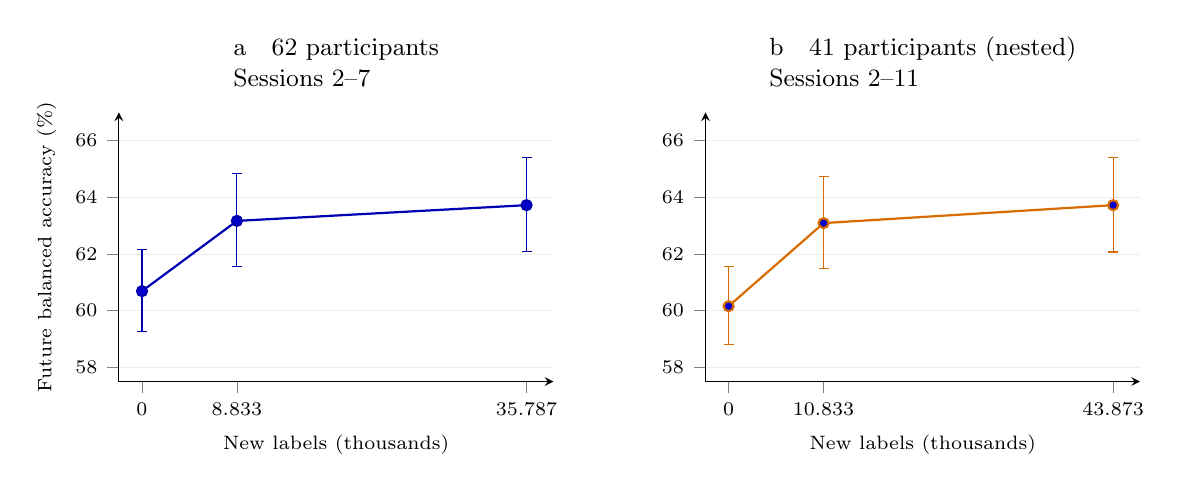
\begin{tikzpicture}
\begin{axis}[axis lines=left,tick align=outside,tick label style={font=\scriptsize},label style={font=\scriptsize},title style={font=\small,align=left},grid style={gray!15},every axis plot/.append style={line width=.8pt},enlarge x limits=false,at={(0.00cm,0)},anchor=north west,width=7.1cm,height=5.0cm,title={a\quad 62 participants\\Sessions 2--7},xlabel={New labels (thousands)},ylabel={Future balanced accuracy (\%)},xmin=-2.14722,xmax=38.29209,ymin=57.5,ymax=67,ytick={58,60,62,64,66},xtick={0,8.833,35.787},xticklabels={0,8.833,35.787},ymajorgrids=true]
\addplot+[blue!70!black,mark=*,mark size=1.8pt,error bars/.cd,y dir=both,y explicit] coordinates {(0,60.6917443602) += (0,1.45751901244) -= (0,1.41353913505) (8.833,63.1704692362) += (0,1.65773709412) -= (0,1.60203707047) (35.787,63.7262091486) += (0,1.67019092038) -= (0,1.62356299933)};
\end{axis}
\begin{axis}[axis lines=left,tick align=outside,tick label style={font=\scriptsize},label style={font=\scriptsize},title style={font=\small,align=left},grid style={gray!15},every axis plot/.append style={line width=.8pt},enlarge x limits=false,at={(7.45cm,0)},anchor=north west,width=7.1cm,height=5.0cm,title={b\quad 41 participants (nested)\\Sessions 2--11},xlabel={New labels (thousands)},ylabel={},xmin=-2.63238,xmax=46.94411,ymin=57.5,ymax=67,ytick={58,60,62,64,66},xtick={0,10.833,43.873},xticklabels={0,10.833,43.873},ymajorgrids=true]
\addplot+[orange!85!black,mark=*,mark size=1.8pt,error bars/.cd,y dir=both,y explicit] coordinates {(0,60.1600324689) += (0,1.40122618041) -= (0,1.34098243433) (10.833,63.0925643526) += (0,1.65786736391) -= (0,1.60640403413) (43.873,63.7263207083) += (0,1.67416690137) -= (0,1.65335726707)};
\end{axis}
\end{tikzpicture}
\caption{Classification performance across the actual new-label budgets in Stieger. Future sessions are averaged within each participant before computing the equal-participant mean. (a) All 62 participants through session 7. (b) The nested 41 participants through session 11. Reduced and all-label conditions use 8,833/35,787 and 10,833/43,873 new labels, respectively; horizontal positions reflect the actual counts. Bars show the original conditional 95\% intervals for cohort means rather than pairwise differences. These conditions use no new high-channel pairs. At each label budget, the separate classifier is identical across pairing schedules. The 41-person cohort provides longer follow-up for a subset of participants and is not an independent replication. Figure~\ref{fig:eeg-pairing-timing} reports the mapping schedule comparisons.}
\label{fig:eeg-budget-calibration}
\end{figure}

Future gains compare the reduced-label classifier with its zero-new-label control, whereas retention compares the final classifier with its own initialization on the same permanent old test. In the 62-participant cohort, the mean old-test change was $+1.392$ percentage points (95\% conditional interval $[-1.468,+4.087]$). Nineteen participants declined, including twelve with declines of at least five points. All nineteen also showed a positive future gain against the zero-label control. Figure~\ref{fig:retention-heterogeneity} reports all participants and their initial eligibility categories. Twenty-nine of 62 met the initial task criterion, and 25 met both the task and target criteria. Results for the nested longer-follow-up cohort and the loss-threshold sensitivity analysis are reported in Appendix~\ref{sec:retention-extended}. The fixed old tests contained 8--38 trials per participant. For 25 of 62 participants, at least one class contained at most ten trials, so a single correctness flip in that class changes balanced accuracy by at least five percentage points when the other predictions are held fixed. The complete class counts and paired changes are reported in Tables~\ref{tab:old-test-resolution} and~\ref{tab:old-test-paired-flips}.

\begin{figure}[t]
\centering
\begingroup
\definecolor{ret0}{HTML}{0072B2}
\definecolor{ret1}{HTML}{56B4E9}
\definecolor{ret2}{HTML}{E69F00}
\definecolor{ret3}{HTML}{B6BBC2}
\definecolor{retgreen}{HTML}{009E73}
\definecolor{retred}{HTML}{D55E00}
\begin{tikzpicture}[font=\scriptsize]
\begin{axis}[width=14.7cm,height=3.2cm,at={(0,0)},anchor=north west,xmin=0,xmax=64,ymin=-.55,ymax=1.55,ytick={0,1},yticklabels={Nested 41,All 62},xtick={0,10,20,30,40,50,60},xlabel={Number of participants},axis lines=left,tick label style={font=\scriptsize},label style={font=\scriptsize},title={A\quad Initial eligibility: all participants retained},title style={at={(0,1.2)},anchor=south west},clip=false]
\path[fill=ret0,draw=white,line width=.3pt] (axis cs:0,0.71) rectangle (axis cs:25,1.29);
\node[font=\scriptsize,text=white] at (axis cs:12.5,1){25};
\path[fill=ret1,draw=white,line width=.3pt] (axis cs:25,0.71) rectangle (axis cs:29,1.29);
\node[font=\scriptsize,text=black] at (axis cs:27,1){4};
\path[fill=ret2,draw=white,line width=.3pt] (axis cs:29,0.71) rectangle (axis cs:55,1.29);
\node[font=\scriptsize,text=black] at (axis cs:42,1){26};
\path[fill=ret3,draw=white,line width=.3pt] (axis cs:55,0.71) rectangle (axis cs:62,1.29);
\node[font=\scriptsize,text=black] at (axis cs:58.5,1){7};
\path[fill=ret0,draw=white,line width=.3pt] (axis cs:0,-0.29) rectangle (axis cs:16,0.29);
\node[font=\scriptsize,text=white] at (axis cs:8,0){16};
\path[fill=ret1,draw=white,line width=.3pt] (axis cs:16,-0.29) rectangle (axis cs:19,0.29);
\node[font=\scriptsize,text=black] at (axis cs:17.5,0){3};
\path[fill=ret2,draw=white,line width=.3pt] (axis cs:19,-0.29) rectangle (axis cs:34,0.29);
\node[font=\scriptsize,text=black] at (axis cs:26.5,0){15};
\path[fill=ret3,draw=white,line width=.3pt] (axis cs:34,-0.29) rectangle (axis cs:41,0.29);
\node[font=\scriptsize,text=black] at (axis cs:37.5,0){7};
\node[anchor=west,font=\scriptsize] at (axis description cs:0.03,1.07){\textcolor{ret0}{\rule{6pt}{6pt}} Task + target};
\node[anchor=west,font=\scriptsize] at (axis description cs:0.275,1.07){\textcolor{ret1}{\rule{6pt}{6pt}} Task only};
\node[anchor=west,font=\scriptsize] at (axis description cs:0.52,1.07){\textcolor{ret2}{\rule{6pt}{6pt}} Target only};
\node[anchor=west,font=\scriptsize] at (axis description cs:0.765,1.07){\textcolor{ret3}{\rule{6pt}{6pt}} Neither};
\end{axis}
\begin{axis}[width=7.2cm,height=6.25cm,at={(0cm,-3.8cm)},anchor=north west,xmin=-8,xmax=8,ymin=-60,ymax=40,xtick={-8,-4,0,4,8},ytick={-60,-40,-20,0,20,40},xlabel={Future BA gain vs 0\% labels (pp)},tick label style={font=\scriptsize},label style={font=\scriptsize},axis lines=left,grid=major,grid style={gray!15},title={B\quad All 62: sessions 2--7},title style={at={(0,1.03)},anchor=south west},ylabel={Permanent-old BA change (pp)}]
\path[fill=red!4] (axis cs:-8,-60) rectangle (axis cs:8,-5);
\addplot[gray,thin,forget plot] coordinates {(-8,0)(8,0)};
\addplot[gray,thin,forget plot] coordinates {(0,-60)(0,40)};
\addplot[retred,dashed,thin,forget plot] coordinates {(-8,-5)(8,-5)};
\addplot[only marks,mark=*,mark size=1.45pt,color=ret0,mark options={draw=white,line width=.2pt}] coordinates {(3.080186945,21.37254902) (6.529490733,-8.391608392) (2.722129871,4.545454545) (4.45990119,3.571428571) (1.311701014,-3.333333333) (2.261738206,6.25) (3.927758534,0.5555555556) (4.483221284,5) (4.00394052,-12.25961538) (2.694509939,1.041666667) (4.541387595,-19.375) (3.33931136,4.358974359) (3.767575336,-3.75) (0.9943816088,0) (0.9701408588,5.882352941) (2.518043685,22.5) (2.768075864,5.263157895) (4.538187236,6.25) (0.965886423,4.545454545) (0.3546783501,12.5) (3.485035405,-10.71428571) (3.174872062,0) (1.872203146,-3.125) (-0.1474877323,6.25) (1.052853246,-8.823529412)};
\addplot[only marks,mark=*,mark size=1.45pt,color=ret1,mark options={draw=white,line width=.2pt}] coordinates {(2.523690368,8.823529412) (2.261157279,12.5) (2.966210377,12.5) (0.4743751473,-6.274509804)};
\addplot[only marks,mark=*,mark size=1.45pt,color=ret2,mark options={draw=white,line width=.2pt}] coordinates {(2.106139182,-6.25) (4.089334812,0) (0.01777891563,-54.54545455) (2.69902457,4.278074866) (-0.3406792357,1.428571429) (2.570327455,0) (5.231051377,10.06493506) (2.372395354,-10) (4.673817429,-11.9047619) (0.03305435487,10.71428571) (4.914845789,3.333333333) (2.767607319,-4.166666667) (6.468992526,0) (1.240423265,5) (0.826416011,-2.222222222) (3.980335038,6.666666667) (5.582603673,8.333333333) (3.200927733,0) (4.249476981,0) (3.294201231,0) (2.878419139,-7.142857143) (3.861439932,-10) (-7.395031554,0) (3.757319443,-4.166666667) (-0.9508436394,3.125) (2.275656643,14.58333333)};
\addplot[only marks,mark=*,mark size=1.45pt,color=ret3,mark options={draw=white,line width=.2pt}] coordinates {(1.671703914,4.545454545) (2.099247332,4.166666667) (-0.5308599236,4.276315789) (4.26770375,17.15686275) (2.577722041,0.6944444444) (0.439360651,-2.631578947) (0.8558749527,33.33333333)};
\addplot[only marks,mark=+,mark size=3.7pt,black,very thick] coordinates {(2.478724876,1.392478139)};
\node[anchor=north west,align=left,fill=white,inner sep=2pt,font=\scriptsize] at (rel axis cs:.025,.98){Old decline: 19/62\\Loss $\geq5$ pp: 12/62};
\node[anchor=west,align=left,font=\tiny,text=gray!80!black] at (axis cs:-7.7,-43){ID 5: old test has\\11 / 1 trials by class};
\draw[gray,thin] (axis cs:-3.6,-46) -- (axis cs:0.01777891563,-54.54545455);
\end{axis}
\begin{axis}[width=7.2cm,height=6.25cm,at={(7.45cm,-3.8cm)},anchor=north west,xmin=-8,xmax=8,ymin=-60,ymax=40,xtick={-8,-4,0,4,8},ytick={-60,-40,-20,0,20,40},xlabel={Future BA gain vs 0\% labels (pp)},tick label style={font=\scriptsize},label style={font=\scriptsize},axis lines=left,grid=major,grid style={gray!15},title={C\quad Nested 41: sessions 2--11},title style={at={(0,1.03)},anchor=south west}]
\path[fill=red!4] (axis cs:-8,-60) rectangle (axis cs:8,-5);
\addplot[gray,thin,forget plot] coordinates {(-8,0)(8,0)};
\addplot[gray,thin,forget plot] coordinates {(0,-60)(0,40)};
\addplot[retred,dashed,thin,forget plot] coordinates {(-8,-5)(8,-5)};
\addplot[only marks,mark=*,mark size=1.45pt,color=ret0,mark options={draw=white,line width=.2pt}] coordinates {(5.237375062,-2.678571429) (4.756905041,0) (5.135951032,8.080808081) (0.6720441272,7.692307692) (4.415810323,4.545454545) (4.510341718,3.333333333) (5.334330317,-2.163461538) (0.7346032967,-8.333333333) (3.11850923,-9.791666667) (3.430773076,-0.625) (0.8316619589,2.941176471) (2.877244539,-8.333333333) (5.090711292,6.666666667) (1.280507079,10) (4.567902958,-10.09615385) (-1.144507079,12.5)};
\addplot[only marks,mark=*,mark size=1.45pt,color=ret1,mark options={draw=white,line width=.2pt}] coordinates {(2.477847297,-5.263157895) (2.987610994,0) (2.939609878,-7.142857143)};
\addplot[only marks,mark=*,mark size=1.45pt,color=ret2,mark options={draw=white,line width=.2pt}] coordinates {(5.756969725,3.095238095) (2.206415117,10) (3.97020147,-4.545454545) (4.486134434,12.66233766) (0.9014493269,-14.54545455) (2.732144943,12.5) (-0.04667536161,3.571428571) (5.547750893,12.5) (3.322789064,4.487179487) (2.499786608,0) (3.019221062,-11.11111111) (1.938745633,7.692307692) (5.014190742,0) (3.786607436,11.22807018) (3.28212599,3.787878788)};
\addplot[only marks,mark=*,mark size=1.45pt,color=ret3,mark options={draw=white,line width=.2pt}] coordinates {(0.9497578182,4.545454545) (1.712987116,4.166666667) (2.236635666,15.625) (4.020001717,3.333333333) (3.571381491,12.5) (0.006530878232,15.55555556) (0.06342332281,0)};
\addplot[only marks,mark=+,mark size=3.7pt,black,very thick] coordinates {(2.932531884,2.643430292)};
\node[anchor=north west,align=left,fill=white,inner sep=2pt,font=\scriptsize] at (rel axis cs:.025,.98){Old decline: 12/41\\Loss $\geq5$ pp: 8/41};
\node[anchor=south east,font=\scriptsize] at (rel axis cs:.97,.04){$+$ Cohort mean};
\end{axis}
\end{tikzpicture}
\endgroup
\caption{Initial eligibility and individual retention in the first fixed Stieger budget experiment. (A) Diagnostic categories are mutually exclusive. Task eligibility requires balanced accuracy (BA) of at least 0.60; target eligibility requires prediction MSE below the actual initial-mean predictor. Task/target/joint counts are 29/51/25 of 62 and 19/31/16 of the nested 41. (B,C) Each point represents one participant, with all eligibility groups included. Both policies receive the same 40 early calibration pairs. The horizontal axis compares approximately 25\% with 0\% new labels, averaging future sessions within each participant; the vertical axis compares the final updated classifier with its own initialization on the same permanently excluded old test. Pairing schedules leave the separate task classifier unchanged. Colors identify the diagnostic categories, black crosses show participant means, and the dashed line marks a five-percentage-point (pp) old-test loss. All 19 old-test declines in the 62-person cohort and all 12 in the nested cohort coexist with positive future gains. The largest decline is included without axis truncation; its old test contains 11 and 1 trials in the two classes. The 41 participants form a subset of the larger cohort and do not provide an independent replication.}
\label{fig:retention-heterogeneity}
\end{figure}

\subsection{Training-risk constraints and the joint retention criterion}
\label{sec:retention-constraints}

The personal-update experiments evaluated a separate retention intervention using matched feedback identities. Both the teacher--candidate line and full-space optimization satisfied their initial-training constraint. Performance on the permanent old test provided a held-out endpoint. Table~\ref{tab:retention-primary} reports future and old-loss differences relative to the unconstrained personal model within each stage.

Both constrained updates met future-performance tolerance in both Stieger cohorts, but neither met the joint criterion. The line-stage old-loss interval crossed zero, while the full-space upper bound equaled zero and therefore failed the strictly negative-bound requirement. Allowing updates in the full coefficient space addressed the geometric restriction of the line; training feasibility still did not establish the specified reduction in excluded-test loss. Complete penalty, replay, source, Farabbi, and training-only diagnostics are reported in Appendix~\ref{sec:retention-extended}, Figure~\ref{fig:retention-tradeoffs}.

\begin{table}[tbp]
\centering\small
\caption{Training-risk constraints in Stieger 62. Each difference compares the constrained update with the unconstrained personal update from the same stage. Entries are in percentage points with conditional 95\% participant-bootstrap intervals. The line row uses the original line-stage interval, and the full-space row uses the later full-space-stage interval. These within-stage contrasts do not compare the two constrained methods with each other or with the shared budget classifier.}
\label{tab:retention-primary}
\begin{tabularx}{\linewidth}{@{}>{\raggedright\arraybackslash}p{.19\linewidth}>{\raggedright\arraybackslash}X>{\raggedright\arraybackslash}X>{\raggedright\arraybackslash}p{.16\linewidth}@{}}
\toprule
Constraint & Future BA difference & Old-loss proportion difference & Joint criterion\\
\midrule
Teacher--candidate line & $+0.411$\newline $[+0.085,+0.721]$ & $-8.065$\newline $[-17.742,+1.613]$ & Not met\\
\addlinespace
Full coefficient space & $+0.070$\newline $[-0.040,+0.194]$ & $-3.226$\newline $[-8.065,0]$ & Not met\\
\bottomrule
\end{tabularx}
\par\smallskip
\begin{minipage}{\linewidth}\footnotesize\raggedright
Old loss is a decline of at least five BA percentage points relative to each model's initialization. The joint rule requires a future lower bound of at least $-0.5$ points and an old-loss-proportion upper bound strictly below zero. Both rows meet future tolerance; neither confirms reduced old-test loss.
\end{minipage}
\end{table}

\section{Discussion}

\subsection{Paired calibration and downstream classification}

With matched calibration budgets, true pairs improved fixed-classifier AUC over class-preserving shuffled pairs, demonstrating the value of exact correspondence beyond task-class grouping for this mapping. The frozen reference asks a different question: whether additional pairs improve an already fitted mapping. That classification gain remained unconfirmed. Relative to frozen mapping, positive participant-level AUC changes were more frequent, but larger declines in a minority outweighed their combined gains.

Feature error and classification weight the predicted channels differently. MSE averages squared errors across omitted-channel coordinates; the fixed classifier combines those coordinates through its discriminant coefficients. Lower overall error can therefore leave the class-relevant score ordering unimproved. Direct low-channel classification benefited from task labels, and omitted-channel prediction benefited from paired measurements. Measuring both endpoints identifies the function that gains from each update. Appendix~\ref{sec:lee-diagnostics} characterizes component error and discriminant alignment in the 12-participant development mappings.

\subsection{Future performance and individual retention}

The Stieger budget experiment improved mean future classification over zero new labels using 75.3\% fewer new labels than the all-label condition. Mean accuracy remained below the all-label condition, defining the measured trade-off between the number of new labels and future performance.

Individual retention changes the interpretation of the mean future gain. All nineteen participants with old-test declines had positive future point differences against the zero-new-label control. The two changes use distinct references: future performance compares label budgets, whereas retention compares the updated model with its own initialization. Their coexistence identifies a retention outcome that the future mean alone would miss. Initial eligibility records starting performance, and the retention distribution includes all participants. Participant heterogeneity is also documented in SMR-BCI calibration and feedback performance \cite{sannelli2019}.

Continual-learning evaluation distinguishes forgetting of earlier tasks from difficulty learning new tasks \cite{chaudhry2018,delange2022}. In class-incremental classification, iCaRL combines a bounded exemplar memory with distillation and representation learning \cite{rebuffi2017}. These approaches specify the update objective, memory budget, and function to be retained. Here, task classes remain fixed, and retention is evaluated within each participant by rescoring the permanently excluded initial test after later-session updates.

Both training-risk constraints met future tolerance, but neither confirmed a reduction in the proportion of participants with old-test declines of at least five percentage points. The constraints bound balanced cross-entropy on initial-training trials; the retention endpoint measures balanced accuracy on permanently excluded trials. Successful optimization therefore establishes feasibility for the training objective, while the old test evaluates retention on different samples and a different loss.

Full-space optimization retained the initial-training risk requirement while allowing updates beyond the teacher--candidate line. Appendix~\ref{app:math} states the generalization condition connecting empirical feasibility to population risk; the training-only controls in Appendix~\ref{sec:retention-extended} examine how the fitted constraints generalize within the initial data.

\subsection{Scope of the evidence}

The findings apply to the fixed readouts and evaluation protocols used here. Lee's original-event results come from the 42-person group held out from protocol development; its 12-person component diagnostics and history-compatible event set retain separate roles. Stieger provides development evidence, with the longer 41-person cohort nested within the larger cohort. Individual old-test changes refer to the fixed excluded trials. Their class counts and paired prediction changes are reported in Tables~\ref{tab:old-test-resolution} and~\ref{tab:old-test-paired-flips}.

Appendix~\ref{app:eeg} reports the complete Yang, Farabbi, history, and feedback-source comparisons. The constructed-state and reliability-reference studies in Appendices~\ref{app:simulation} and~\ref{app:reliability} quantify the effects of observation access, inference settings, and correctness-sequence assumptions. These analyses concern specified model behavior; the main EEG results concern classification and retention on the recorded tasks.

\section{Conclusion}

Task labels and paired recordings improved different prediction functions under the tested low-channel EEG protocols. In Lee, correct pairing improved omitted-channel prediction and fixed-classifier AUC relative to class-preserving shuffles, while the classification gain over frozen mapping remained unconfirmed. In Stieger, reduced-label updating improved mean future classification over zero new labels, alongside individual old-test declines relative to each model's initialization. Training-risk constraints met future tolerance but left reduced old-test loss unconfirmed. These results make the choice of reference model and retention test central to interpreting adaptation gains. Matched information budgets, explicit feedback timing, and individual old-test changes provide a reproducible basis for evaluating which functions benefit from adaptation and which earlier performance is retained.

\paragraph{Data and computational materials.}
The original EEG datasets are publicly available through their source publications and repositories \cite{stieger2021,lee2019,yang2025,farabbi2020}. Study-specific materials are available in version v1.1.0 of \href{https://github.com/Yiming-S/low-channel-eeg-adaptation/releases/tag/v1.1.0}{the accompanying GitHub release}. The archived-results package contains saved result records, compact participant endpoints for the principal comparisons, paired-trial inputs for the original Stieger reduced-label old-test comparison, frozen protocols, available experiment implementations, and statistical-methods records. The documented entry points in \texttt{paper/reproducibility/} and \texttt{paper/reviewer\_revision/} regenerate the scientific figures, independently recompute the principal participant-bootstrap statistics and added descriptive summaries, and check reported-value pointers and file hashes. The release was tested after extraction outside the research checkout. Preprocessing and model reruns require separate raw EEG, encoder weights, feature caches, and fitted-model or trial-prediction arrays. Those pipelines are inventoried in the package, while the archived-results checks evaluate the saved results.

\appendix

\section{Conditional-information identity and empirical retention}
\label{app:math}

\subsection{Conditional information and observability}

For an optimal squared-error predictor, the benefit of additional information can be expressed precisely. If information sets satisfy $\mathcal F\subseteq\mathcal G$ and $Z$ has a finite second moment, then
\begin{equation}
 \E\|Z-\E(Z\mid\mathcal F)\|^2-
 \E\|Z-\E(Z\mid\mathcal G)\|^2
 =\E\|\E(Z\mid\mathcal G)-\E(Z\mid\mathcal F)\|^2\geq0.
 \label{eq:information}
\end{equation}
The identity quantifies the gain for optimal conditional-mean prediction. Equality holds when the two information sets yield the same conditional mean. The derivation below also connects empirical retention constraints to population risk under a deviation condition.

Observability describes whether output behavior can distinguish different internal states \cite{hermann1977}. For a linear system with transition $A$ and observation map $C$, a past state direction affects low-channel observations through $C,CA,CA^2,\ldots$. If a direction remains unobservable, additional recordings of the same low-channel view cannot identify changes along that direction. Our simulations include both this case and systems in which hidden coordinates influence subsequent low-channel observations.

\subsection{Derivation and retention condition}

Let $m_F=\E(Z\mid\mathcal F)$ and $m_G=\E(Z\mid\mathcal G)$, with $\mathcal F\subseteq\mathcal G$. Writing $Z-m_F=(Z-m_G)+(m_G-m_F)$ and using $\E(Z-m_G\mid\mathcal G)=0$ gives
\begin{align*}
 \E\|Z-m_F\|^2
 &=\E\|Z-m_G\|^2+\E\|m_G-m_F\|^2\\
 &\quad+2\E\{(Z-m_G)^\top(m_G-m_F)\}\\
 &=\E\|Z-m_G\|^2+\E\|m_G-m_F\|^2.
\end{align*}
The final term is zero because $m_G-m_F$ is measurable with respect to $\mathcal G$. For fitted predictors, realized performance additionally depends on approximation and estimation errors.

For retention, suppose a fitted model satisfies $\widehat R_0(\theta)\leq\widehat R_0(\theta_0)+\epsilon$ on initial training data. If a uniform deviation bound $|R_0(\vartheta)-\widehat R_0(\vartheta)|\leq\eta$ holds for both $\vartheta=\theta$ and $\theta_0$, then
\begin{equation}
 R_0(\theta)-R_0(\theta_0)\leq\epsilon+2\eta.
\end{equation}
The population-risk bound combines empirical feasibility with the stated deviation condition. In the EEG experiments, the constraint uses training cross-entropy, and the permanent old test evaluates held-out task performance through balanced accuracy.

\section{Extended EEG endpoints and analysis identity}
\label{app:eeg}

\begin{table}[tbp]
\centering\small
\caption{Evidence index for the information-to-function comparisons. Each row specifies the evaluation population, endpoint, and evidence role. The corresponding results and appendix tables report the exact estimates and decision boundaries.}
\label{tab:contrasts}
\begin{tabularx}{\linewidth}{@{}>{\raggedright\arraybackslash}p{.17\linewidth}>{\raggedright\arraybackslash}p{.28\linewidth}>{\raggedright\arraybackslash}p{.25\linewidth}>{\raggedright\arraybackslash}X@{}}
\toprule
Question & Comparison and endpoint & Evaluation & Evidence role\\
\midrule
Mapped prediction and task benefit & True pairs versus frozen/class-preserving shuffled mapping; omitted-channel MSE and fixed mapped AUC & Lee 42; original-event future test & Fixed additional-participant evaluation; descriptive 95\% contrasts\\
\addlinespace
Initial-function retention & Old-test loss relative to each model's initialization; constrained versus unconstrained updates for future tolerance and harm reduction & Stieger and Farabbi permanent initial tests & Development retention comparisons with fixed operational criteria\\
\addlinespace
Budget and alignment & Label counts for BA; true versus within-class shuffled pairs for target NMSE & Stieger; later Yang mapping control & Development; later mapping diagnostics on existing datasets\\
\addlinespace
Ordered history & Ordered/current/timing versus current/timing and shuffled history; AUC & Lee 42; common legal events & Two fixed 97.5\% confirmation contrasts\\
\addlinespace
Feedback source & Other or mixed versus personal feedback; future BA & Stieger and Farabbi; recipient label counts matched & Stieger development and fixed Farabbi direction test\\
\addlinespace
Information and update location & Observable coupling, update component, parameter measurements; state MSE & Known-state paths with paired noise realizations & Mechanism controls and finite-algorithm diagnostics\\
\addlinespace
Reliability interpretation & Fixed versus sampled correctness and persistence; defined failure event & Saved teacher-based correctness reference & Assumption sensitivity; separate from deployed EEG failure rates\\
\bottomrule
\end{tabularx}
\end{table}

\subsection{Extended datasets and model specifications}

\paragraph{Yang.}
The two-class subset comprises 51 participants with three sessions \cite{yang2025}; the separate three-class group is excluded by design. The high-channel view contains 59 documented EEG channels, whereas the low-channel view uses C3/C4. In session 1, original blocks 1--3 are used for initial fitting, block 4 for diagnosis without hyperparameter selection, and block 5 for the permanent old test. All eligible low-view labels from session 2 are released after that session's prediction barrier; only the first original block supplies 40 planned high-channel pairs per participant. Session 3 provides the future test, with no subsequent update. All 51 planned participants remain in the analysis. The original Yang joint-model procedure and hyperparameters were fixed before acquisition and evaluation of its outcomes. The original procedure is therefore independent of this project's downstream development; whether Yang was included in REVE's pretraining data remains unestablished.

\paragraph{Farabbi.}
The public dataset contains 12 participants recorded on three consecutive days using 32 EEG electrodes \cite{farabbi2020}. We include all 12 available participants and analyze the first-person training recordings specified in the protocol. The task combines prompted left/right motor imagery with robot-action observation, so this is not a pure mental-imagery replication of Stieger. For each participant and class, a fixed random half of day 1 trials is assigned to initial training and the remainder to the permanent old test, yielding twenty trials in each subset and ten per class. There is no separate diagnostic split, eligibility criterion, or lifetime endpoint in this experiment. All six methods use C3/C4, without consuming a high-channel view or paired-calibration budget. Each receiving personal model uses ten new feedback trials under the matched-source conditions after prediction on day 2. Day 3 is evaluated without a terminal update. The subsequent training-only diagnostic analyses are development studies and do not replace the original confirmation.

For Stieger, Yang, and Farabbi, the frozen REVE-base encoder produces a 512-dimensional mean-pooled representation from channel and temporal tokens \cite{reve2025}. In Stieger and Yang, low- and high-channel representations are extracted independently from their permitted channel sets; Farabbi uses only the low representation. The encoder is not fine-tuned. Predictions are made at the trial level using the complete specified epoch, rather than sample by sample. Stieger uses cue-locked windows from 0 to 3\,s, resampling from 1,000 to 200\,Hz before channelwise fourth-order 0.5--95\,Hz zero-phase filtering within the window. Yang uses the three seconds from 1.5 to 4.5\,s after cue onset, resampling to 200\,Hz before fourth-order 0.5--95\,Hz filtering within the trial. Farabbi uses 0--3\,s after the cue, fourth-order 0.5--75\,Hz filtering within the window, and resampling from 250 to 200\,Hz. All three datasets undergo within-window, channelwise population standardization and clipping to $[-15,15]$, with the recorded reference retained. Raw physical units are checked before scaling. The reference and normalization statistics for a low-channel view are computed without using unobserved high channels.

The original joint model uses an affine map $\widehat Z=WX+b$ and a task head with logit $v^\top\widehat Z+c$. The source and accumulated target-domain balanced binary cross-entropy terms each have weight 0.5. The initial and new pairing losses each receive half of the structure-loss weight. Unavailable information contributes a zero term, without renormalizing the remaining terms. Head regularization and displacement from the initial adapter use coefficient 0.001. Initial development selected a structure weight of 0.3 and a ridge penalty of 0.1 from fixed candidate grids; these values were subsequently reused for Yang. Fits use full-batch double-precision L-BFGS with recorded objective and gradient diagnostics. Optimizer termination alone is not taken to establish a global solution of the factorized joint objective.

The later direct classifiers are initialized using class-balanced initial-training cross-entropy plus $0.001\|w\|^2/2$. Once feedback is released, pooled initial-training and cumulative released-feedback losses each have weight 0.5, with the same regularizer and an unpenalized intercept. Source comparisons use the same pooled initial replay. The constraint stages likewise include global initial-data replay and recipient-specific feedback in the objective; the functional risk constraint is evaluated on the recipient's own initial-training trials. The independent ridge pairing experiment weights initial and new pair losses by 0.5 each. The budget experiment weights them by 0.25 each when new pairs are present, preserving its baseline total data weight. The objectives were fixed separately and define different mapping updates.

For the REVE target, participant-specific NMSE divides target MSE by the frozen mean per-coordinate population variance of that participant's initial-training target. Mean-predictor skill uses the actual error of the fixed initial target mean on those same evaluation trials. An NMSE of one therefore does not imply that the mapping matches the current test error of the mean predictor. Lee reports MSE in its own fixed initial standardized ERP coordinates.

For the extended source contrasts, recipients are resampled while fitted teachers and realized donor assignments remain fixed. Each of the Stieger 62 source, Farabbi source, and Lee history-confirmation families contains two main contrasts. Their original Bonferroni rule uses a two-sided 97.5\% interval for each contrast, corresponding to a nominal family error rate of 0.05. Source contrasts in the nested Stieger 41 cohort use descriptive 95\% intervals. The earliest archived joint-model EEG analysis used 5,000 participant resamples with seed 20261002; the later EEG stages use 10,000. The stage registry in \texttt{paper/reproducibility/statistical\_methods.json} specifies the seed derivations and recorded runtime evidence for each analysis.

\subsection{Pair budgets, timing, and alignment}
\label{sec:paired}

In the nested 41-participant cohort, future accuracies under the label budgets were 60.160\%, 63.093\%, and 63.726\% for zero, reduced, and all new labels, respectively. The target-mapping pathway is evaluated separately below.

In the separate mapping experiment, forty early pairs per participant reduced future target MSE from 0.245743 to 0.225210 in the 62-participant cohort. Uniform and late allocations yielded 0.225257 and 0.233147. The separate classifier was identical across pairing schedules at a given label budget, by construction. The experiment therefore establishes a mapping benefit alongside a separately measured feedback benefit, but not a classification benefit from the pairs. Figure~\ref{fig:eeg-pairing-timing} shows the actual label counts and the separate schedule comparison at equal pair budgets for both follow-up horizons.

\begin{figure}[p]
\centering
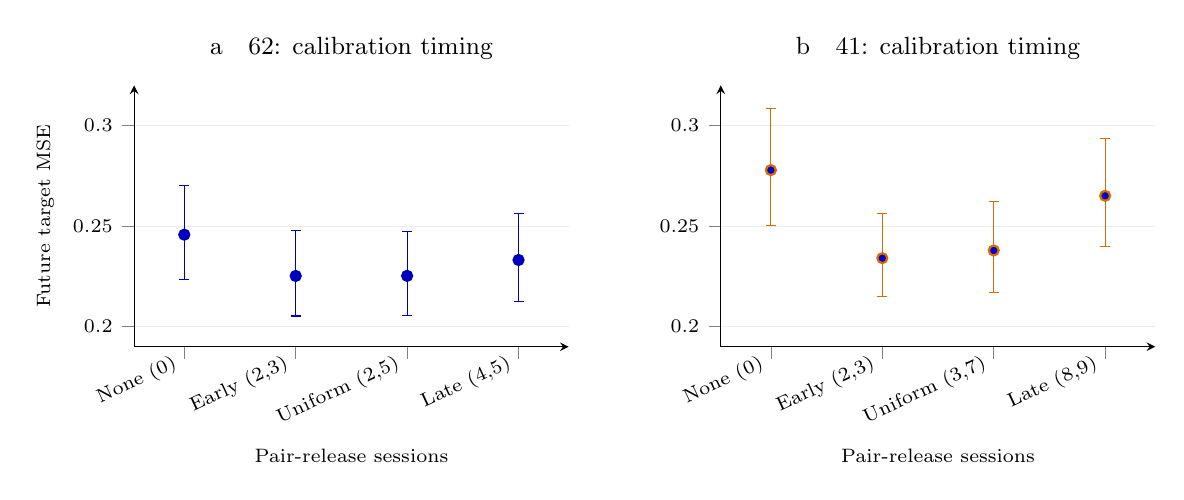
\begin{tikzpicture}
\begin{axis}[axis lines=left,tick align=outside,tick label style={font=\scriptsize},label style={font=\scriptsize},title style={font=\small,align=left},grid style={gray!15},every axis plot/.append style={line width=.8pt},enlarge x limits=false,at={(0.00cm,0)},anchor=north west,width=7.1cm,height=4.9cm,title={a\quad 62: calibration timing},xlabel={Pair-release sessions},ylabel={Future target MSE},xmin=-.45,xmax=3.45,ymin=.19,ymax=.32,xtick={0,1,2,3},xticklabels={{None (0)},{Early (2,3)},{Uniform (2,5)},{Late (4,5)}},x tick label style={font=\scriptsize,rotate=25,anchor=east},ymajorgrids=true]
\addplot+[blue!70!black,only marks,mark=*,mark size=1.8pt,error bars/.cd,y dir=both,y explicit] coordinates {(0,0.245743243314) += (0,0.024570447724) -= (0,0.0221293726146) (1,0.22520983582) += (0,0.022493893387) -= (0,0.0199498372161) (2,0.225256572168) += (0,0.0220335955838) -= (0,0.0198270007915) (3,0.233147015323) += (0,0.0230862874186) -= (0,0.0207748232485)};
\end{axis}
\begin{axis}[axis lines=left,tick align=outside,tick label style={font=\scriptsize},label style={font=\scriptsize},title style={font=\small,align=left},grid style={gray!15},every axis plot/.append style={line width=.8pt},enlarge x limits=false,at={(7.45cm,0)},anchor=north west,width=7.1cm,height=4.9cm,title={b\quad 41: calibration timing},xlabel={Pair-release sessions},ylabel={},xmin=-.45,xmax=3.45,ymin=.19,ymax=.32,xtick={0,1,2,3},xticklabels={{None (0)},{Early (2,3)},{Uniform (3,7)},{Late (8,9)}},x tick label style={font=\scriptsize,rotate=25,anchor=east},ymajorgrids=true]
\addplot+[orange!85!black,only marks,mark=*,mark size=1.8pt,error bars/.cd,y dir=both,y explicit] coordinates {(0,0.27786084499) += (0,0.0306096249832) -= (0,0.0273798011893) (1,0.234050541004) += (0,0.0220115240923) -= (0,0.0190929894667) (2,0.237877427954) += (0,0.0245181808356) -= (0,0.0211244328039) (3,0.265071637858) += (0,0.0285627311323) -= (0,0.025104375337)};
\end{axis}
\end{tikzpicture}
\caption{Separate mapping calibration at equal follow-up pair budgets in Stieger. (a) All 62 participants; (b) the nested 41 with longer follow-up. Each active schedule releases two batches of 20 pairs per participant; release sessions are shown in parentheses, and the zero-pair reference has a different budget. No new task labels enter these mapping arms. The mapping schedule does not change the separate task classifier. Bars show the original conditional 95\% intervals for cohort means computed with equal participant weights. These comparisons evaluate the specified allocations rather than an optimal calibration interval.}
\label{fig:eeg-pairing-timing}
\end{figure}

The original Yang joint-model protocol was fixed before this project downloaded or evaluated the recordings. The ridge pairing control below was specified separately, after earlier outcomes from these cohorts were known. It provides a descriptive alignment diagnostic on the existing datasets, rather than an independent confirmation.

The later independent ridge control evaluated the contribution of exact alignment beyond class information. In Stieger, true pairs minus the average of shuffled pairs reduced normalized target MSE by 0.10005 (95\% interval $[-0.11774,-0.08117]$). The nested longer-follow-up result was $-0.08857$ ($[-0.10603,-0.07097]$). The Stieger comparisons use sessions 4 onward, after the first scheduled pairing release. In the Yang session 3 test, the corresponding difference was $+0.27237$ ($[-0.04413,+0.86741]$). This descriptive comparison did not confirm an advantage of same-trial pairs in Yang. The pairing-control experiment contains no classification model, so these normalized-error differences do not establish a task-accuracy benefit. Figure~\ref{fig:eeg-pairing-forest} shows the group contrasts alongside the number of participants with lower or higher target error, while distinguishing the nested cohort. In Yang, 30 of 51 participants had lower error with true pairs even though the equal-participant mean contrast was positive; the full distribution retains the large positive tail.

\begin{figure}[t]
\centering
\resizebox{14.8cm}{!}{%
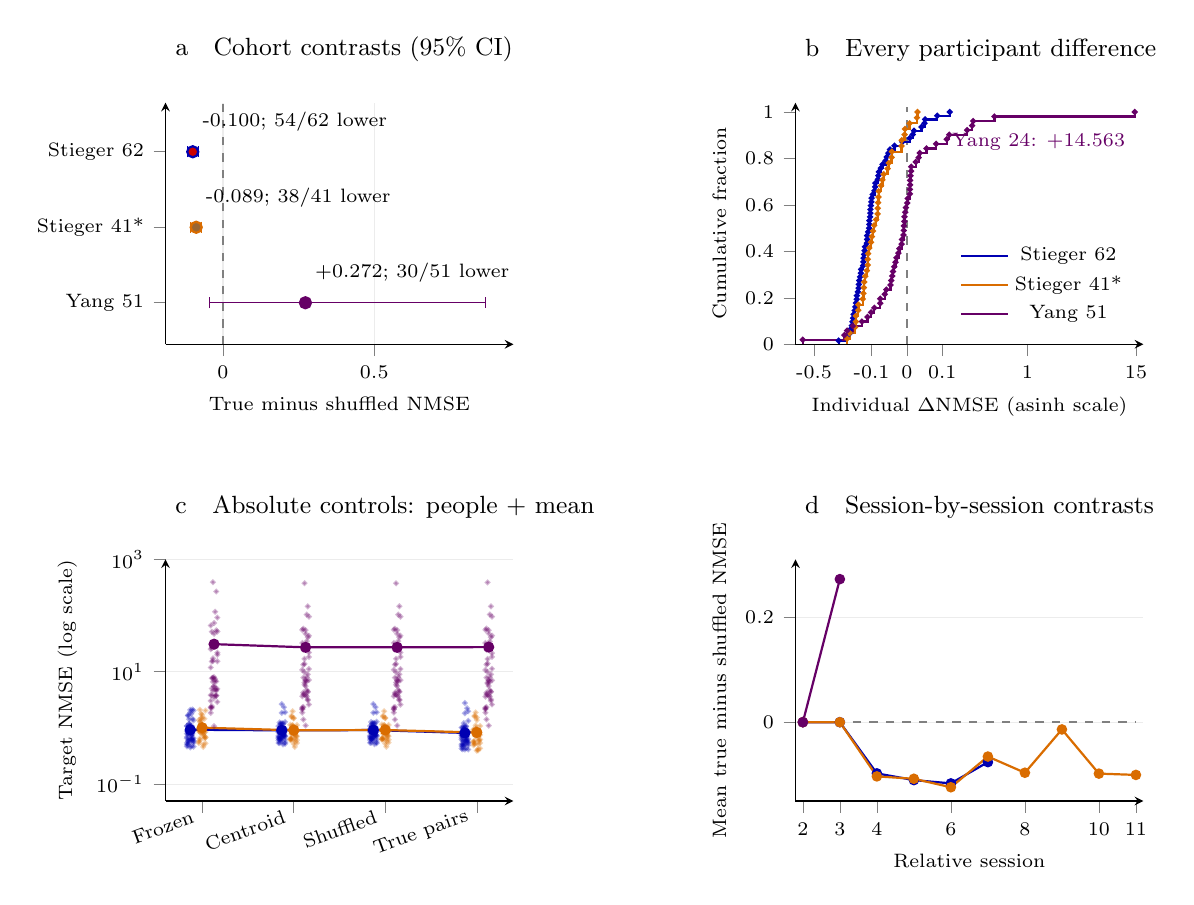
\begin{tikzpicture}
\begin{axis}[axis lines=left,tick align=outside,tick label style={font=\scriptsize},label style={font=\scriptsize},title style={font=\small,align=left},grid style={gray!15},every axis plot/.append style={line width=.8pt},enlarge x limits=false,at={(0cm,0cm)},anchor=north west,width=6.0cm,height=4.65cm,title={a\quad Cohort contrasts (95\% CI)},title style={font=\small,align=left,at={(0,1.06)},anchor=south west},xlabel={True minus shuffled NMSE},xmin=-.19,xmax=.96,ymin=-.55,ymax=2.65,ytick={2,1,0},yticklabels={Stieger 62,Stieger 41*,Yang 51},xmajorgrids=true]
\addplot[gray,dashed] coordinates {(0,-0.55) (0,2.65)};
\addplot+[blue!70!black,only marks,mark=*,error bars/.cd,x dir=both,x explicit] coordinates {(-0.100050350785,2) += (0.0188769171113,0) -= (0.0176857672942,0)};
\node[anchor=south west,font=\scriptsize] at (axis cs:-0.100050350785,2.14) {-0.100; 54/62 lower};
\addplot+[orange!85!black,only marks,mark=*,error bars/.cd,x dir=both,x explicit] coordinates {(-0.088566965314,1) += (0.0176001594016,0) -= (0.017458614644,0)};
\node[anchor=south west,font=\scriptsize] at (axis cs:-0.088566965314,1.1400000000000001) {-0.089; 38/41 lower};
\addplot+[violet!80!black,only marks,mark=*,error bars/.cd,x dir=both,x explicit] coordinates {(0.272372634248,0) += (0.595035209948,0) -= (0.316502448873,0)};
\node[anchor=south west,font=\scriptsize] at (axis cs:0.272372634248,0.14) {+0.272; 30/51 lower};
\end{axis}
\begin{axis}[axis lines=left,tick align=outside,tick label style={font=\scriptsize},label style={font=\scriptsize},title style={font=\small,align=left},grid style={gray!15},every axis plot/.append style={line width=.8pt},enlarge x limits=false,at={(8.0cm,0cm)},anchor=north west,width=6.0cm,height=4.65cm,title={b\quad Every participant difference},title style={font=\small,align=left,at={(0,1.06)},anchor=south west},xlabel={Individual $\Delta$NMSE (asinh scale)},ylabel={Cumulative fraction},ymin=0,ymax=1.04,xmin=-2.77647,xmax=5.88688,xtick={-2.31243834127,-0.88137358702,0,0.88137358702,2.9982229503,5.70379358558},xticklabels={-0.5,-0.1,0,0.1,1,15},legend style={font=\scriptsize,at={(.98,.04)},anchor=south east,draw=none}]
\addplot[gray,dashed,forget plot] coordinates {(0,0) (0,1.02)};
\addplot[blue!70!black,no marks] coordinates {(-1.70085226732,0) (-1.70085226732,0.0161290322581) (-1.50421970302,0.0161290322581) (-1.50421970302,0.0322580645161) (-1.41223660492,0.0322580645161) (-1.41223660492,0.0483870967742) (-1.40841939414,0.0483870967742) (-1.40841939414,0.0645161290323) (-1.37226147835,0.0645161290323) (-1.37226147835,0.0806451612903) (-1.35517188974,0.0806451612903) (-1.35517188974,0.0967741935484) (-1.34218314146,0.0967741935484) (-1.34218314146,0.112903225806) (-1.32676852528,0.112903225806) (-1.32676852528,0.129032258065) (-1.29969204144,0.129032258065) (-1.29969204144,0.145161290323) (-1.28560528512,0.145161290323) (-1.28560528512,0.161290322581) (-1.26805281647,0.161290322581) (-1.26805281647,0.177419354839) (-1.24969515175,0.177419354839) (-1.24969515175,0.193548387097) (-1.24873025127,0.193548387097) (-1.24873025127,0.209677419355) (-1.22339284622,0.209677419355) (-1.22339284622,0.225806451613) (-1.20290451273,0.225806451613) (-1.20290451273,0.241935483871) (-1.19755899353,0.241935483871) (-1.19755899353,0.258064516129) (-1.18769684376,0.258064516129) (-1.18769684376,0.274193548387) (-1.16660555474,0.274193548387) (-1.16660555474,0.290322580645) (-1.14814231758,0.290322580645) (-1.14814231758,0.306451612903) (-1.14061598207,0.306451612903) (-1.14061598207,0.322580645161) (-1.09041710884,0.322580645161) (-1.09041710884,0.338709677419) (-1.08734150854,0.338709677419) (-1.08734150854,0.354838709677) (-1.08153039545,0.354838709677) (-1.08153039545,0.370967741935) (-1.06658711272,0.370967741935) (-1.06658711272,0.387096774194) (-1.05672731297,0.387096774194) (-1.05672731297,0.403225806452) (-1.04497686413,0.403225806452) (-1.04497686413,0.41935483871) (-0.996862818381,0.41935483871) (-0.996862818381,0.435483870968) (-0.99095933346,0.435483870968) (-0.99095933346,0.451612903226) (-0.990530396769,0.451612903226) (-0.990530396769,0.467741935484) (-0.966461163532,0.467741935484) (-0.966461163532,0.483870967742) (-0.943396140303,0.483870967742) (-0.943396140303,0.5) (-0.937063331253,0.5) (-0.937063331253,0.516129032258) (-0.93340167435,0.516129032258) (-0.93340167435,0.532258064516) (-0.9185244334,0.532258064516) (-0.9185244334,0.548387096774) (-0.911616273687,0.548387096774) (-0.911616273687,0.564516129032) (-0.908525169458,0.564516129032) (-0.908525169458,0.58064516129) (-0.900053186957,0.58064516129) (-0.900053186957,0.596774193548) (-0.886574886711,0.596774193548) (-0.886574886711,0.612903225806) (-0.881015331811,0.612903225806) (-0.881015331811,0.629032258065) (-0.851580065326,0.629032258065) (-0.851580065326,0.645161290323) (-0.807971436168,0.645161290323) (-0.807971436168,0.661290322581) (-0.792045930975,0.661290322581) (-0.792045930975,0.677419354839) (-0.786441396196,0.677419354839) (-0.786441396196,0.693548387097) (-0.722645645716,0.693548387097) (-0.722645645716,0.709677419355) (-0.712353933566,0.709677419355) (-0.712353933566,0.725806451613) (-0.697737511513,0.725806451613) (-0.697737511513,0.741935483871) (-0.651314642921,0.741935483871) (-0.651314642921,0.758064516129) (-0.606692922714,0.758064516129) (-0.606692922714,0.774193548387) (-0.530674259932,0.774193548387) (-0.530674259932,0.790322580645) (-0.504651524739,0.790322580645) (-0.504651524739,0.806451612903) (-0.463004631924,0.806451612903) (-0.463004631924,0.822580645161) (-0.422787293399,0.822580645161) (-0.422787293399,0.838709677419) (-0.310770227518,0.838709677419) (-0.310770227518,0.854838709677) (-0.115067711201,0.854838709677) (-0.115067711201,0.870967741935) (0.0677194054936,0.870967741935) (0.0677194054936,0.887096774194) (0.1445303758,0.887096774194) (0.1445303758,0.903225806452) (0.175642806438,0.903225806452) (0.175642806438,0.91935483871) (0.360485739608,0.91935483871) (0.360485739608,0.935483870968) (0.438931116076,0.935483870968) (0.438931116076,0.951612903226) (0.452774912034,0.951612903226) (0.452774912034,0.967741935484) (0.755336082752,0.967741935484) (0.755336082752,0.983870967742) (1.06682822103,0.983870967742) (1.06682822103,1)};
\addplot[blue!70!black,only marks,mark=*,mark size=.65pt,forget plot] coordinates {(-1.70085226732,0.0161290322581) (-1.50421970302,0.0322580645161) (-1.41223660492,0.0483870967742) (-1.40841939414,0.0645161290323) (-1.37226147835,0.0806451612903) (-1.35517188974,0.0967741935484) (-1.34218314146,0.112903225806) (-1.32676852528,0.129032258065) (-1.29969204144,0.145161290323) (-1.28560528512,0.161290322581) (-1.26805281647,0.177419354839) (-1.24969515175,0.193548387097) (-1.24873025127,0.209677419355) (-1.22339284622,0.225806451613) (-1.20290451273,0.241935483871) (-1.19755899353,0.258064516129) (-1.18769684376,0.274193548387) (-1.16660555474,0.290322580645) (-1.14814231758,0.306451612903) (-1.14061598207,0.322580645161) (-1.09041710884,0.338709677419) (-1.08734150854,0.354838709677) (-1.08153039545,0.370967741935) (-1.06658711272,0.387096774194) (-1.05672731297,0.403225806452) (-1.04497686413,0.41935483871) (-0.996862818381,0.435483870968) (-0.99095933346,0.451612903226) (-0.990530396769,0.467741935484) (-0.966461163532,0.483870967742) (-0.943396140303,0.5) (-0.937063331253,0.516129032258) (-0.93340167435,0.532258064516) (-0.9185244334,0.548387096774) (-0.911616273687,0.564516129032) (-0.908525169458,0.58064516129) (-0.900053186957,0.596774193548) (-0.886574886711,0.612903225806) (-0.881015331811,0.629032258065) (-0.851580065326,0.645161290323) (-0.807971436168,0.661290322581) (-0.792045930975,0.677419354839) (-0.786441396196,0.693548387097) (-0.722645645716,0.709677419355) (-0.712353933566,0.725806451613) (-0.697737511513,0.741935483871) (-0.651314642921,0.758064516129) (-0.606692922714,0.774193548387) (-0.530674259932,0.790322580645) (-0.504651524739,0.806451612903) (-0.463004631924,0.822580645161) (-0.422787293399,0.838709677419) (-0.310770227518,0.854838709677) (-0.115067711201,0.870967741935) (0.0677194054936,0.887096774194) (0.1445303758,0.903225806452) (0.175642806438,0.91935483871) (0.360485739608,0.935483870968) (0.438931116076,0.951612903226) (0.452774912034,0.967741935484) (0.755336082752,0.983870967742) (1.06682822103,1)};
\addplot[orange!85!black,no marks] coordinates {(-1.48966947563,0) (-1.48966947563,0.0243902439024) (-1.42577014244,0.0243902439024) (-1.42577014244,0.0487804878049) (-1.29247875516,0.0487804878049) (-1.29247875516,0.0731707317073) (-1.27213272968,0.0731707317073) (-1.27213272968,0.0975609756098) (-1.27186532111,0.0975609756098) (-1.27186532111,0.121951219512) (-1.21137568526,0.121951219512) (-1.21137568526,0.146341463415) (-1.2084000258,0.146341463415) (-1.2084000258,0.170731707317) (-1.10021372552,0.170731707317) (-1.10021372552,0.19512195122) (-1.08388034142,0.19512195122) (-1.08388034142,0.219512195122) (-1.07526653214,0.219512195122) (-1.07526653214,0.243902439024) (-1.06198085861,0.243902439024) (-1.06198085861,0.268292682927) (-1.03978874717,0.268292682927) (-1.03978874717,0.292682926829) (-0.998889045846,0.292682926829) (-0.998889045846,0.317073170732) (-0.977324298616,0.317073170732) (-0.977324298616,0.341463414634) (-0.97598732501,0.341463414634) (-0.97598732501,0.365853658537) (-0.968850926161,0.365853658537) (-0.968850926161,0.390243902439) (-0.936419295594,0.390243902439) (-0.936419295594,0.414634146341) (-0.894342608565,0.414634146341) (-0.894342608565,0.439024390244) (-0.873007851582,0.439024390244) (-0.873007851582,0.463414634146) (-0.844933035589,0.463414634146) (-0.844933035589,0.487804878049) (-0.816317236504,0.487804878049) (-0.816317236504,0.512195121951) (-0.767331946304,0.512195121951) (-0.767331946304,0.536585365854) (-0.730668518075,0.536585365854) (-0.730668518075,0.560975609756) (-0.72869085728,0.560975609756) (-0.72869085728,0.585365853659) (-0.717928846778,0.585365853659) (-0.717928846778,0.609756097561) (-0.709281707067,0.609756097561) (-0.709281707067,0.634146341463) (-0.703792479773,0.634146341463) (-0.703792479773,0.658536585366) (-0.646010694087,0.658536585366) (-0.646010694087,0.682926829268) (-0.611509861443,0.682926829268) (-0.611509861443,0.707317073171) (-0.578045823137,0.707317073171) (-0.578045823137,0.731707317073) (-0.482985269663,0.731707317073) (-0.482985269663,0.756097560976) (-0.454600731875,0.756097560976) (-0.454600731875,0.780487804878) (-0.382232771892,0.780487804878) (-0.382232771892,0.80487804878) (-0.373747269517,0.80487804878) (-0.373747269517,0.829268292683) (-0.137868701276,0.829268292683) (-0.137868701276,0.853658536585) (-0.130015004755,0.853658536585) (-0.130015004755,0.878048780488) (-0.0599291148048,0.878048780488) (-0.0599291148048,0.90243902439) (-0.0471002093283,0.90243902439) (-0.0471002093283,0.926829268293) (0.0654785066784,0.926829268293) (0.0654785066784,0.951219512195) (0.249643738245,0.951219512195) (0.249643738245,0.975609756098) (0.261593736465,0.975609756098) (0.261593736465,1)};
\addplot[orange!85!black,only marks,mark=*,mark size=.65pt,forget plot] coordinates {(-1.48966947563,0.0243902439024) (-1.42577014244,0.0487804878049) (-1.29247875516,0.0731707317073) (-1.27213272968,0.0975609756098) (-1.27186532111,0.121951219512) (-1.21137568526,0.146341463415) (-1.2084000258,0.170731707317) (-1.10021372552,0.19512195122) (-1.08388034142,0.219512195122) (-1.07526653214,0.243902439024) (-1.06198085861,0.268292682927) (-1.03978874717,0.292682926829) (-0.998889045846,0.317073170732) (-0.977324298616,0.341463414634) (-0.97598732501,0.365853658537) (-0.968850926161,0.390243902439) (-0.936419295594,0.414634146341) (-0.894342608565,0.439024390244) (-0.873007851582,0.463414634146) (-0.844933035589,0.487804878049) (-0.816317236504,0.512195121951) (-0.767331946304,0.536585365854) (-0.730668518075,0.560975609756) (-0.72869085728,0.585365853659) (-0.717928846778,0.609756097561) (-0.709281707067,0.634146341463) (-0.703792479773,0.658536585366) (-0.646010694087,0.682926829268) (-0.611509861443,0.707317073171) (-0.578045823137,0.731707317073) (-0.482985269663,0.756097560976) (-0.454600731875,0.780487804878) (-0.382232771892,0.80487804878) (-0.373747269517,0.829268292683) (-0.137868701276,0.853658536585) (-0.130015004755,0.878048780488) (-0.0599291148048,0.90243902439) (-0.0471002093283,0.926829268293) (0.0654785066784,0.951219512195) (0.249643738245,0.975609756098) (0.261593736465,1)};
\addplot[violet!80!black,no marks] coordinates {(-2.59285645337,0) (-2.59285645337,0.0196078431373) (-1.55899657354,0.0196078431373) (-1.55899657354,0.0392156862745) (-1.49065493737,0.0392156862745) (-1.49065493737,0.0588235294118) (-1.34962372786,0.0588235294118) (-1.34962372786,0.078431372549) (-1.12178134757,0.078431372549) (-1.12178134757,0.0980392156863) (-0.982315066691,0.0980392156863) (-0.982315066691,0.117647058824) (-0.892809078394,0.117647058824) (-0.892809078394,0.137254901961) (-0.813436862651,0.137254901961) (-0.813436862651,0.156862745098) (-0.664288998899,0.156862745098) (-0.664288998899,0.176470588235) (-0.662998267765,0.176470588235) (-0.662998267765,0.196078431373) (-0.553061983257,0.196078431373) (-0.553061983257,0.21568627451) (-0.512574766452,0.21568627451) (-0.512574766452,0.235294117647) (-0.409644624799,0.235294117647) (-0.409644624799,0.254901960784) (-0.390989126956,0.254901960784) (-0.390989126956,0.274509803922) (-0.36513953415,0.274509803922) (-0.36513953415,0.294117647059) (-0.346935831822,0.294117647059) (-0.346935831822,0.313725490196) (-0.316260055477,0.313725490196) (-0.316260055477,0.333333333333) (-0.285185335142,0.333333333333) (-0.285185335142,0.352941176471) (-0.259365967725,0.352941176471) (-0.259365967725,0.372549019608) (-0.212495106267,0.372549019608) (-0.212495106267,0.392156862745) (-0.187444270117,0.392156862745) (-0.187444270117,0.411764705882) (-0.13208316844,0.411764705882) (-0.13208316844,0.43137254902) (-0.124546903191,0.43137254902) (-0.124546903191,0.450980392157) (-0.0860756821715,0.450980392157) (-0.0860756821715,0.470588235294) (-0.0787713975395,0.470588235294) (-0.0787713975395,0.490196078431) (-0.0758518116496,0.490196078431) (-0.0758518116496,0.509803921569) (-0.0636559704622,0.509803921569) (-0.0636559704622,0.529411764706) (-0.058559903812,0.529411764706) (-0.058559903812,0.549019607843) (-0.0433017728286,0.549019607843) (-0.0433017728286,0.56862745098) (-0.026256361804,0.56862745098) (-0.026256361804,0.588235294118) (0.00667378647941,0.588235294118) (0.00667378647941,0.607843137255) (0.0202842917163,0.607843137255) (0.0202842917163,0.627450980392) (0.0732886809423,0.627450980392) (0.0732886809423,0.647058823529) (0.0737631899771,0.647058823529) (0.0737631899771,0.666666666667) (0.077888494639,0.666666666667) (0.077888494639,0.686274509804) (0.078677439391,0.686274509804) (0.078677439391,0.705882352941) (0.0880346224529,0.705882352941) (0.0880346224529,0.725490196078) (0.10319850689,0.725490196078) (0.10319850689,0.745098039216) (0.106595565398,0.745098039216) (0.106595565398,0.764705882353) (0.218840516578,0.764705882353) (0.218840516578,0.78431372549) (0.290747188937,0.78431372549) (0.290747188937,0.803921568627) (0.317521601755,0.803921568627) (0.317521601755,0.823529411765) (0.486024041803,0.823529411765) (0.486024041803,0.843137254902) (0.724711379966,0.843137254902) (0.724711379966,0.862745098039) (0.991620837562,0.862745098039) (0.991620837562,0.882352941176) (1.05119731649,0.882352941176) (1.05119731649,0.901960784314) (1.49905679797,0.901960784314) (1.49905679797,0.921568627451) (1.62280714302,0.921568627451) (1.62280714302,0.941176470588) (1.65001199503,0.941176470588) (1.65001199503,0.960784313725) (2.17766417426,0.960784313725) (2.17766417426,0.980392156863) (5.67422444788,0.980392156863) (5.67422444788,1)};
\addplot[violet!80!black,only marks,mark=*,mark size=.65pt,forget plot] coordinates {(-2.59285645337,0.0196078431373) (-1.55899657354,0.0392156862745) (-1.49065493737,0.0588235294118) (-1.34962372786,0.078431372549) (-1.12178134757,0.0980392156863) (-0.982315066691,0.117647058824) (-0.892809078394,0.137254901961) (-0.813436862651,0.156862745098) (-0.664288998899,0.176470588235) (-0.662998267765,0.196078431373) (-0.553061983257,0.21568627451) (-0.512574766452,0.235294117647) (-0.409644624799,0.254901960784) (-0.390989126956,0.274509803922) (-0.36513953415,0.294117647059) (-0.346935831822,0.313725490196) (-0.316260055477,0.333333333333) (-0.285185335142,0.352941176471) (-0.259365967725,0.372549019608) (-0.212495106267,0.392156862745) (-0.187444270117,0.411764705882) (-0.13208316844,0.43137254902) (-0.124546903191,0.450980392157) (-0.0860756821715,0.470588235294) (-0.0787713975395,0.490196078431) (-0.0758518116496,0.509803921569) (-0.0636559704622,0.529411764706) (-0.058559903812,0.549019607843) (-0.0433017728286,0.56862745098) (-0.026256361804,0.588235294118) (0.00667378647941,0.607843137255) (0.0202842917163,0.627450980392) (0.0732886809423,0.647058823529) (0.0737631899771,0.666666666667) (0.077888494639,0.686274509804) (0.078677439391,0.705882352941) (0.0880346224529,0.725490196078) (0.10319850689,0.745098039216) (0.106595565398,0.764705882353) (0.218840516578,0.78431372549) (0.290747188937,0.803921568627) (0.317521601755,0.823529411765) (0.486024041803,0.843137254902) (0.724711379966,0.862745098039) (0.991620837562,0.882352941176) (1.05119731649,0.901960784314) (1.49905679797,0.921568627451) (1.62280714302,0.941176470588) (1.65001199503,0.960784313725) (2.17766417426,0.980392156863) (5.67422444788,1)};
\node[anchor=north east,font=\scriptsize,text=violet!80!black] at (axis cs:5.67422444788,.95) {Yang 24: +14.563};
\legend{Stieger 62,Stieger 41*,Yang 51}
\end{axis}
\begin{axis}[axis lines=left,tick align=outside,tick label style={font=\scriptsize},label style={font=\scriptsize},title style={font=\small,align=left},grid style={gray!15},every axis plot/.append style={line width=.8pt},enlarge x limits=false,at={(0cm,-5.8cm)},anchor=north west,width=6.0cm,height=4.65cm,title={c\quad Absolute controls: people + mean},title style={font=\small,align=left,at={(0,1.06)},anchor=south west},ymode=log,ymin=.05,ymax=1000,xmin=-.4,xmax=3.4,xtick={0,1,2,3},xticklabels={Frozen,Centroid,Shuffled,True pairs},x tick label style={font=\scriptsize,rotate=20,anchor=east},ylabel={Target NMSE (log scale)},ymajorgrids=true]
\addplot[blue!70!black,only marks,mark=*,mark size=.6pt,opacity=.28,forget plot] coordinates {(-0.166,0.502893492787) (-0.154,0.565143543266) (-0.142,0.551473513599) (-0.13,1.00798309006) (-0.118,0.732566740523) (-0.106,0.785733681802) (-0.094,2.03810661329) (-0.166,0.654561607494) (-0.154,0.810970446158) (-0.142,1.16287439465) (-0.13,0.93853414505) (-0.118,0.745337332915) (-0.106,2.12343124747) (-0.094,0.937757532446) (-0.166,1.08200051219) (-0.154,1.65682873998) (-0.142,0.628081906431) (-0.13,0.906060637123) (-0.118,1.77325689224) (-0.106,0.855868339572) (-0.094,0.578549468107) (-0.166,1.07149620537) (-0.154,0.896499514633) (-0.142,0.869824788983) (-0.13,0.824385999969) (-0.118,0.475020895594) (-0.106,0.650936838917) (-0.094,0.463469076395) (-0.166,0.467015224432) (-0.154,0.595196465341) (-0.142,1.42788892144) (-0.13,1.11351439149) (-0.118,0.97585623203) (-0.106,0.864154835952) (-0.094,0.54186519757) (-0.166,0.874835205603) (-0.154,0.842527471425) (-0.142,0.869508057105) (-0.13,0.626403729464) (-0.118,0.748714371941) (-0.106,1.45334652319) (-0.094,0.656436357875) (-0.166,0.689586000042) (-0.154,0.505859509974) (-0.142,1.19685006812) (-0.13,0.449315513576) (-0.118,0.631588527372) (-0.106,0.613359220969) (-0.094,0.594156719246) (-0.166,0.787767683752) (-0.154,1.68202952481) (-0.142,1.02849488759) (-0.13,2.09714293249) (-0.118,1.09013447237) (-0.106,0.848871625395) (-0.094,1.35860662435) (-0.166,0.539076699892) (-0.154,0.76273703861) (-0.142,0.869290741153) (-0.13,1.89870359253) (-0.118,0.613508751695) (-0.106,0.870424207131)};
\addplot[blue!70!black,only marks,mark=*,mark size=.6pt,opacity=.28,forget plot] coordinates {(0.834,0.599486614407) (0.846,0.63662720976) (0.858,0.611229283095) (0.87,0.844719888467) (0.882,0.78794573459) (0.894,0.812558352038) (0.906,1.89980947405) (0.834,0.720157427562) (0.846,0.827633723657) (0.858,0.915926937678) (0.87,0.645378555968) (0.882,0.741326946496) (0.894,2.33284215282) (0.906,0.946970505799) (0.834,0.83390787771) (0.846,0.87868630257) (0.858,0.675219433141) (0.87,0.88951950964) (0.882,1.15889754689) (0.894,0.831041794164) (0.906,0.623208721801) (0.834,1.07177871897) (0.846,0.881402616848) (0.858,0.995014410806) (0.87,0.929605738038) (0.882,0.508660794128) (0.894,0.716475544695) (0.906,0.523112231138) (0.834,0.53859151255) (0.846,0.68640406924) (0.858,1.18681662978) (0.87,1.21009764506) (0.882,0.720323038747) (0.894,0.891227760312) (0.906,0.554833852278) (0.834,0.939547886051) (0.846,0.874953346673) (0.858,0.644232791102) (0.87,0.71052475482) (0.882,0.803928509043) (0.894,1.0148074968) (0.906,0.702491711152) (0.834,0.653101588578) (0.846,0.537466196918) (0.858,1.15050139261) (0.87,0.582227316512) (0.882,0.759861127746) (0.894,0.745013354536) (0.906,0.719676769962) (0.834,0.879270693579) (0.846,1.25229082804) (0.858,1.08829178571) (0.87,2.64900165342) (0.882,1.2020017355) (0.894,0.821731587603) (0.906,1.2793362687) (0.834,0.685150092921) (0.846,0.624395692076) (0.858,0.872270021243) (0.87,1.85051411212) (0.882,0.713355128698) (0.894,0.748573303047)};
\addplot[blue!70!black,only marks,mark=*,mark size=.6pt,opacity=.28,forget plot] coordinates {(1.834,0.607202257508) (1.846,0.64662954513) (1.858,0.623044537465) (1.87,0.85288324376) (1.882,0.804126613673) (1.894,0.820705140559) (1.906,1.89553393485) (1.834,0.728225674528) (1.846,0.835109602885) (1.858,0.922821710842) (1.87,0.651240613464) (1.882,0.748056578689) (1.894,2.33941410728) (1.906,0.956442250675) (1.834,0.842024903737) (1.846,0.887173769376) (1.858,0.68307328995) (1.87,0.899479438613) (1.882,1.17188683408) (1.894,0.83920274268) (1.906,0.62943272719) (1.834,1.0808010413) (1.846,0.893291768248) (1.858,1.00578384885) (1.87,0.941682448061) (1.882,0.514468655999) (1.894,0.725963915398) (1.906,0.530617204742) (1.834,0.544775157324) (1.846,0.693202879493) (1.858,1.19866336064) (1.87,1.22381492867) (1.882,0.734405596722) (1.894,0.899266283397) (1.906,0.561651935931) (1.834,0.949619139546) (1.846,0.884145546849) (1.858,0.653373335491) (1.87,0.719745306595) (1.882,0.813835516956) (1.894,1.03423262855) (1.906,0.711275828992) (1.834,0.661007888455) (1.846,0.543009800549) (1.858,1.15956787016) (1.87,0.593566479165) (1.882,0.769570716653) (1.894,0.755336094769) (1.906,0.72918110683) (1.834,0.891701932765) (1.846,1.27101435704) (1.858,1.09782043063) (1.87,2.65208294615) (1.882,1.21606556442) (1.894,0.829807626971) (1.906,1.28740831549) (1.834,0.695251210398) (1.846,0.636235642994) (1.858,0.880622883985) (1.87,1.85803362968) (1.882,0.72497484232) (1.894,0.757753798898)};
\addplot[blue!70!black,only marks,mark=*,mark size=.6pt,opacity=.28,forget plot] coordinates {(2.834,0.475230325345) (2.846,0.51856627357) (2.858,0.491581238469) (2.87,0.867386652242) (2.882,0.652653933472) (2.894,0.72075579908) (2.906,1.97845763576) (2.834,0.620729095243) (2.846,0.729785453949) (2.858,0.959656125302) (2.87,0.502510787631) (2.882,0.695421964501) (2.894,2.23553695917) (2.906,0.853782955809) (2.834,0.752145344801) (2.846,0.736669166761) (2.858,0.582336359098) (2.87,0.851506889385) (2.882,1.07605651171) (2.894,0.795653160725) (2.906,0.552017901299) (2.834,1.01634082849) (2.846,0.748309165884) (2.858,0.845649501654) (2.87,0.771904892269) (2.882,0.438894072445) (2.894,0.601382276211) (2.906,0.41358060028) (2.834,0.428645302002) (2.846,0.585167981352) (2.858,1.21631809153) (2.87,1.00989243754) (2.882,0.621995657906) (2.894,0.812260952388) (2.906,0.491816895265) (2.834,0.840649799763) (2.846,0.753639880963) (2.858,0.512919689888) (2.87,0.603681175954) (2.882,0.709512168705) (2.894,0.855926854592) (2.906,0.632555352721) (2.834,0.667785006119) (2.846,0.41654236397) (2.858,1.07181827873) (2.87,0.412590257686) (2.882,0.594395143324) (2.894,0.563088247561) (2.906,0.536104664367) (2.834,0.728074598274) (2.846,1.00621001946) (2.858,0.956065135141) (2.87,2.78018539705) (2.882,1.0561133097) (2.894,0.818275446318) (2.906,1.3327244781) (2.834,0.510714834136) (2.846,0.469216975873) (2.858,0.825029384676) (2.87,1.826453959) (2.882,0.569751379084) (2.894,0.804594244664)};
\addplot[blue!70!black,mark=*,mark size=1.6pt] coordinates {(-0.13,0.927006685854) (0.87,0.905354124194) (1.87,0.914650628758) (2.87,0.814600277974)};
\addplot[orange!85!black,only marks,mark=*,mark size=.6pt,opacity=.28,forget plot] coordinates {(-0.036,0.539089074711) (-0.024,0.603432916675) (-0.012,1.19732607424) (0,1.71262435989) (0.012,0.795076079077) (0.024,1.04813060291) (0.036,2.03785535717) (-0.036,0.916409652447) (-0.024,0.838939938681) (-0.012,1.79142199966) (0,1.11970632689) (0.012,1.06314885602) (0.024,1.45839953948) (0.036,0.684100353894) (-0.036,0.970231847294) (-0.024,2.1055437835) (-0.012,0.805101005547) (0,0.930287151883) (0.012,0.502715970007) (0.024,0.710317406938) (0.036,0.530664589899) (-0.036,0.573155026167) (-0.024,0.648830534081) (-0.012,1.48523431568) (0,1.53593846729) (0.012,0.914449456577) (0.024,0.831961723807) (0.036,0.669881043204) (-0.036,0.881829029905) (-0.024,0.954046934566) (-0.012,1.34713074181) (0,0.888607742584) (0.012,0.458493846457) (0.024,0.651192028952) (0.036,0.852068617274) (-0.036,1.38568063652) (-0.024,1.28223971948) (-0.012,1.04758147687) (0,0.839759132899) (0.012,0.746812316801) (0.024,1.01196515931)};
\addplot[orange!85!black,only marks,mark=*,mark size=.6pt,opacity=.28,forget plot] coordinates {(0.964,0.61045826536) (0.976,0.648999758383) (0.988,0.906707292318) (1,1.49748050433) (1.012,0.749782227925) (1.024,0.922661766454) (1.036,1.11816999414) (0.964,0.643017333014) (0.976,0.781219426098) (0.988,1.97613132489) (1,1.0474722539) (1.012,0.88961605157) (1.024,1.00063309596) (1.036,0.70669329692) (0.964,0.944922046634) (0.976,1.56437833803) (0.988,0.901180199409) (1,0.945663485882) (1.012,0.45767619085) (1.024,0.700289406051) (1.036,0.538250962464) (0.964,0.625804801249) (0.976,0.667491108055) (0.988,1.09951219538) (1,1.48294934763) (1.012,0.839106607292) (1.024,0.832697609833) (1.036,0.607750250309) (0.964,0.909904781533) (0.976,0.611386412034) (0.988,1.01386326342) (1,0.517706113904) (1.012,0.577440375647) (1.024,0.733515369379) (1.036,0.873746769059) (0.964,1.13591491864) (0.976,1.63658139697) (0.988,1.11617203649) (1,0.782141264472) (1.012,0.633940542181) (1.024,0.961455950948)};
\addplot[orange!85!black,only marks,mark=*,mark size=.6pt,opacity=.28,forget plot] coordinates {(1.964,0.617527471765) (1.976,0.65805796102) (1.988,0.915450106802) (2,1.50300908136) (2.012,0.758644880201) (2.024,0.930301001882) (2.036,1.1272391921) (1.964,0.64782939606) (1.976,0.789124216627) (1.988,1.98406473109) (2,1.05740558371) (2.012,0.894720545836) (2.024,1.010738632) (2.036,0.714559095871) (1.964,0.953738357087) (1.976,1.57479625356) (1.988,0.912246279712) (2,0.957592260949) (2.012,0.462932318805) (2.024,0.709044318773) (2.036,0.545816439358) (1.964,0.631244791153) (1.976,0.674197247204) (1.988,1.10943558994) (2,1.49218811762) (2.012,0.847610239306) (2.024,0.842181093276) (2.036,0.615029927765) (1.964,0.92131708758) (1.976,0.619411236696) (1.988,1.02662346671) (2,0.524008110834) (2.012,0.588096691991) (2.024,0.74221089468) (2.036,0.885382466551) (1.964,1.15024896212) (1.976,1.64292423124) (1.988,1.12891996471) (2,0.790100042987) (2.012,0.643831885826) (2.024,0.97148886483)};
\addplot[orange!85!black,only marks,mark=*,mark size=.6pt,opacity=.28,forget plot] coordinates {(2.964,0.493772969804) (2.976,0.530741764071) (2.988,0.90161951885) (3,1.52946783075) (3.012,0.679153604324) (3.024,0.816452704812) (3.036,1.08019704912) (2.964,0.556824553494) (2.976,0.749963367677) (2.988,1.88222217316) (3,0.977661515339) (3.012,0.881682385042) (3.024,0.846379000723) (3.036,0.619647305676) (2.964,0.903540001221) (2.976,1.60002074154) (2.988,0.716209384204) (3,0.805119826729) (3.012,0.397898259281) (3.024,0.610223926928) (3.036,0.431765448452) (2.964,0.5701668898) (2.976,0.589709172189) (2.988,1.10472382734) (3,1.3794183114) (3.012,0.809359287446) (3.024,0.765154427635) (3.036,0.538694990601) (2.964,0.803968324912) (2.976,0.511471126297) (2.988,0.948502410263) (3,0.394529753769) (3.012,0.419736031263) (3.024,0.589195203141) (3.036,0.751782055989) (2.964,0.939739860415) (2.976,1.64947676182) (2.988,0.964508880698) (3,0.784103543606) (3.012,0.512939496902) (3.024,0.902299773018)};
\addplot[orange!85!black,mark=*,mark size=1.6pt] coordinates {(0,1.00896050822) (1,0.907572788659) (2,0.916372903356) (3,0.827805938042)};
\addplot[violet!80!black,only marks,mark=*,mark size=.6pt,opacity=.28,forget plot] coordinates {(0.094,3.82225257698) (0.106,2.42480317499) (0.118,4.57836095087) (0.13,47.3346807032) (0.142,28.6931739019) (0.154,4.58351311228) (0.166,2.90318838061) (0.094,1.85830290174) (0.106,51.379266214) (0.118,7.8250044601) (0.13,73.630999329) (0.142,7.45457872284) (0.154,54.3361049282) (0.166,51.951346877) (0.094,66.4610934661) (0.106,15.1510533417) (0.118,15.634430505) (0.13,3.43876913916) (0.142,27.8758194453) (0.154,267.845907433) (0.166,91.8882693219) (0.094,11.8836322956) (0.106,5.04755489313) (0.118,392.588912629) (0.13,5.5235741916) (0.142,4.8581552441) (0.154,4.87347105648) (0.166,21.8139099394) (0.094,25.3013633303) (0.106,3.83038651027) (0.118,7.72435115403) (0.13,8.0259792684) (0.142,116.771957989) (0.154,3.76275459806) (0.166,20.02719869) (0.094,3.03477333896) (0.106,7.63296460004) (0.118,6.60285910192) (0.13,1.07603533027) (0.142,6.78970983235) (0.154,3.75828406948) (0.166,15.326223013) (0.094,2.35220269741) (0.106,26.5063698352) (0.118,17.3236130577) (0.13,5.48533977722) (0.142,3.77118167897) (0.154,6.75972610989) (0.166,4.94976988018) (0.094,2.27221021497) (0.106,2.28761174568)};
\addplot[violet!80!black,only marks,mark=*,mark size=.6pt,opacity=.28,forget plot] coordinates {(1.094,3.6589607874) (1.106,2.35147561609) (1.118,3.96364768227) (1.13,47.4762869764) (1.142,25.3161575503) (1.154,4.45596153632) (1.166,2.5998501749) (1.094,2.30449936224) (1.106,58.2572113098) (1.118,9.82493248393) (1.13,54.9987245241) (1.142,8.01389325627) (1.154,41.1292197127) (1.166,43.7126286686) (1.094,55.6505077742) (1.106,13.3359730141) (1.118,13.7919626515) (1.13,3.77130709689) (1.142,34.9800399259) (1.154,145.878984881) (1.166,95.6963325554) (1.094,10.7889626658) (1.106,4.26010759394) (1.118,376.238313035) (1.13,6.94573229693) (1.142,4.73476637216) (1.154,4.33940434976) (1.166,21.9471136905) (1.094,32.5692954661) (1.106,3.99385511249) (1.118,6.39211939683) (1.13,7.11661595028) (1.142,104.182481628) (1.154,3.21079810193) (1.166,18.3436310558) (1.094,2.15559375804) (1.106,7.86064695733) (1.118,5.85553984252) (1.13,1.09950935646) (1.142,6.68055697558) (1.154,3.1012558193) (1.166,11.153179663) (1.094,2.17152923084) (1.106,24.5906036631) (1.118,16.9865811471) (1.13,5.54415844253) (1.142,3.63495170677) (1.154,8.98992155786) (1.166,7.09635656864) (1.094,1.87218253113) (1.106,1.40906017312)};
\addplot[violet!80!black,only marks,mark=*,mark size=.6pt,opacity=.28,forget plot] coordinates {(2.094,3.6741275853) (2.106,2.35019232802) (2.118,3.96907173751) (2.13,47.5095704978) (2.142,25.3175749686) (2.154,4.4728547262) (2.166,2.60042620183) (2.094,2.31649582092) (2.106,58.2592620429) (2.118,9.81710938206) (2.13,55.0077118662) (2.142,8.01464812828) (2.154,41.158591024) (2.166,43.7397020666) (2.094,55.6818536872) (2.106,13.3353433291) (2.118,13.7844416183) (2.13,3.76856789513) (2.142,34.987657028) (2.154,145.935727898) (2.166,95.642083259) (2.094,10.8011149108) (2.106,4.2640706613) (2.118,374.579452034) (2.13,6.94320913699) (2.142,4.75781277707) (2.154,4.34051587866) (2.166,22.0210027278) (2.094,32.6293221281) (2.106,4.00050621267) (2.118,6.42559217206) (2.13,7.11940447086) (2.142,104.214804085) (2.154,3.21057248603) (2.166,18.3630332293) (2.094,2.15483623501) (2.106,7.86654387646) (2.118,5.84556412105) (2.13,1.09959210699) (2.142,6.69931182446) (2.154,3.10654386855) (2.166,11.1696990316) (2.094,2.17008063988) (2.106,24.6139239023) (2.118,16.9597465287) (2.13,5.56504684008) (2.142,3.63301896599) (2.154,8.99636902098) (2.166,7.08101451295) (2.094,1.8725023327) (2.106,1.40748175365)};
\addplot[violet!80!black,only marks,mark=*,mark size=.6pt,opacity=.28,forget plot] coordinates {(3.094,3.60270412675) (3.106,2.34756639015) (3.118,3.95582498185) (3.13,47.9451885507) (3.142,25.396558513) (3.154,4.43552396472) (3.166,2.60822292901) (3.094,2.28110205802) (3.106,58.3754933004) (3.118,9.86764798526) (3.13,54.7805267922) (3.142,8.01031659766) (3.154,41.1880771112) (3.166,43.727215152) (3.094,55.5912379245) (3.106,13.3676317272) (3.118,14.0351913523) (3.13,3.72644808224) (3.142,34.8078252011) (3.154,145.724989029) (3.166,95.6206734696) (3.094,10.7298500073) (3.106,4.2554524602) (3.118,389.142398457) (3.13,6.96526828287) (3.142,4.70428112588) (3.154,4.35119563341) (3.166,21.3563479352) (3.094,32.4920911508) (3.106,3.99413631577) (3.118,6.42762074034) (3.13,7.10055008551) (3.142,104.427510246) (3.154,3.2209106641) (3.166,18.3368048573) (3.094,2.16271209853) (3.106,7.85895141964) (3.118,6.08906167323) (3.13,1.10025949059) (3.142,6.58450239707) (3.154,3.04837474648) (3.166,11.295276815) (3.094,2.17741607058) (3.106,24.5817680461) (3.118,16.8581227321) (3.13,5.55716155161) (3.142,3.64040197591) (3.154,8.96746234047) (3.166,7.04091176656) (3.094,1.86664299479) (3.106,1.41629659158)};
\addplot[violet!80!black,mark=*,mark size=1.6pt] coordinates {(0.13,30.9614312737) (1.13,27.1849682676) (2.13,27.1618568934) (3.13,27.4342295276)};
\end{axis}
\begin{axis}[axis lines=left,tick align=outside,tick label style={font=\scriptsize},label style={font=\scriptsize},title style={font=\small,align=left},grid style={gray!15},every axis plot/.append style={line width=.8pt},enlarge x limits=false,at={(8.0cm,-5.8cm)},anchor=north west,width=6.0cm,height=4.65cm,title={d\quad Session-by-session contrasts},title style={font=\small,align=left,at={(0,1.06)},anchor=south west},xlabel={Relative session},ylabel={Mean true minus shuffled NMSE},xmin=1.8,xmax=11.2,ymin=-.15,ymax=.31,xtick={2,3,4,6,8,10,11},ymajorgrids=true]
\addplot[gray,dashed] coordinates {(2,0) (11,0)};
\addplot[blue!70!black,mark=*,mark size=1.5pt] coordinates {(2,1.11022302463e-16) (3,0) (4,-0.0974525821682) (5,-0.110246845599) (6,-0.116516609118) (7,-0.0759853662537)};
\addplot[orange!85!black,mark=*,mark size=1.5pt] coordinates {(2,0) (3,-1.11022302463e-16) (4,-0.10318170685) (5,-0.1077272416) (6,-0.123872892915) (7,-0.0654254755833) (8,-0.0962439595192) (9,-0.0137916131472) (10,-0.0979151864874) (11,-0.10037764641)};
\addplot[violet!80!black,mark=*,mark size=1.5pt] coordinates {(2,0) (3,0.272372634248)};
\end{axis}
\end{tikzpicture}%
}
\caption{Pairing effects across cohorts, participants, controls, and sessions. (a) Original conditional 95\% participant-bootstrap intervals for true pairs minus the mean of five within-class shuffles; labels give the number of participants with lower error. (b) The empirical cumulative distribution includes every participant difference in the primary window. The horizontal transformation is $\operatorname{asinh}(\Delta\mathrm{NMSE}/0.1)$, approximately linear near zero and compressing the tails, with ticks in original NMSE units; Yang participant 24 at $+14.563$ is retained. (c) Small points show individual absolute NMSE values, and connected large points show equal-participant means, on a logarithmic axis. Frozen, class-centroid, shuffled, and true-pair controls use the same fixed target and initial-variance normalizer. (d) Session-specific contrasts use equal participant weights, without newly estimated intervals. Stieger releases pairs after sessions 3, 6, and 9 when available; Yang releases after session 2. Panels (a--c) average future sessions 4--7 for Stieger 62, 4--11 for Stieger 41, and session 3 for Yang. The asterisk marks the nested 41-person cohort; cohorts are not pooled. Shuffled values are within-person means over five assignments, not independent replications. No task classifier is fitted in this experiment.}
\label{fig:eeg-pairing-forest}
\end{figure}

The original Yang joint protocol also revealed a limitation in initialization. No participant met both initial task and structural eligibility (0/51), including the separate-ridge structural pathway. Successful maintenance of an initially demonstrated joint capability therefore cannot be established in this dataset. It does not remove any participant from the primary future comparison. Error reductions from a poor initial mapping must be interpreted alongside actual mean-predictor skill and the unconfirmed matched-shuffle comparison.





\subsection{Lee development component diagnostics}
\label{sec:lee-diagnostics}

Exploratory diagnostics in the 12 previously evaluated Lee development participants distinguished prediction of a component shared across omitted channels from prediction of spatial deviations. After true-pair updating, their mean prediction skills were 0.870 and 0.208, respectively. Mapped scores had a mean correlation of 0.310 with the frozen full-view teacher scores, and the mean mapped-to-teacher class-gap ratio was 0.0972. These diagnostics characterize the development mappings; they do not identify a cause of the AUC result in the separate 42-participant confirmation group. Table~\ref{tab:lee-development-diagnostics} reports the saved diagnostic values and their definitions.

The separate 12-participant development diagnostics characterize predictable channel components and the teacher's task scores (Table~\ref{tab:lee-development-diagnostics}). The shared component was more predictable than spatial deviations. These results describe predictions in the development group; they do not confirm a mechanism in the 42-participant group. A positive rescaling of classifier scores leaves AUC unchanged, so the class-separation ratio alone cannot explain the unconfirmed AUC gain. Their diagnostic value is the joint examination of task-relevant outputs and overall reconstruction error.

\subsection{Ordered low-channel history fails the ERP confirmation criteria}
\label{sec:history}

The original-event and history protocols use different event sets. History comparisons restrict every method to events with the same legal two-second causal history. The confirmation calibration set contains 539--561 such events per participant, totaling 23,012. The ordered-history condition concatenates 32 current ERP features, 32 history features formed from sixteen 125\,ms means per channel, and 19 timing variables. The explicit two-second history ends strictly before flash onset and lies within the same character; the causal filter state can still contain earlier activity. We compare current features, current features plus temporal variables, ordered history with the same temporal variables, and five controls that permute history-bin order while retaining current features and timing. The current-plus-timing and ordered-plus-timing models have 51 and 83 features, respectively. History construction uses only samples available at each flash's prediction time. A high-channel classifier evaluated on the same events provides a separate measurement-information reference using the same allowed fitting labels.

On the common legal event set, label updating with current low-channel features increased future AUC from 0.65660 to 0.68706. The paired difference was 0.03046 (95\% interval $[0.01898,0.04453]$); 41 of 42 participants improved and one declined. These values are computed on the history-compatible event set and therefore differ from the original-event values in Section~\ref{sec:mapped-task}.

The two predefined history comparisons did not confirm an ordered-history benefit. Adding ordered history to current features and temporal variables reduced performance relative to current features with the same temporal variables: AUC difference $-0.004816$, with a 97.5\% interval $[-0.007771,-0.001665]$. The ordered-history condition minus the average shuffled-history control was $+0.002716$, with interval $[-0.000057,+0.005632]$. The first contrast establishes a negative net contribution from this fixed representation; the second leaves the incremental value of ordering unconfirmed.

A full-channel classifier on the identical legal events and allowed labels reached future AUC 0.92398, compared with 0.68706 for current low features. The descriptive 95\% interval for the difference was $[0.21596,0.25803]$ around a mean difference of 0.23692. This establishes a measurement-information gap for these classifiers. It does not define a theoretical upper bound or show that every history representation must fail. Together, the matched current-feature and shuffled-history controls refine the interpretation: the specified two-second history representation did not replace the additional spatial information in this ERP protocol. Figure~\ref{fig:eeg-lee-history} shows all common-history controls and confirmation contrasts; the original-event mapping comparison is separate in Figure~\ref{fig:eeg-lee-endpoints}.



\begin{figure}[p]
\centering
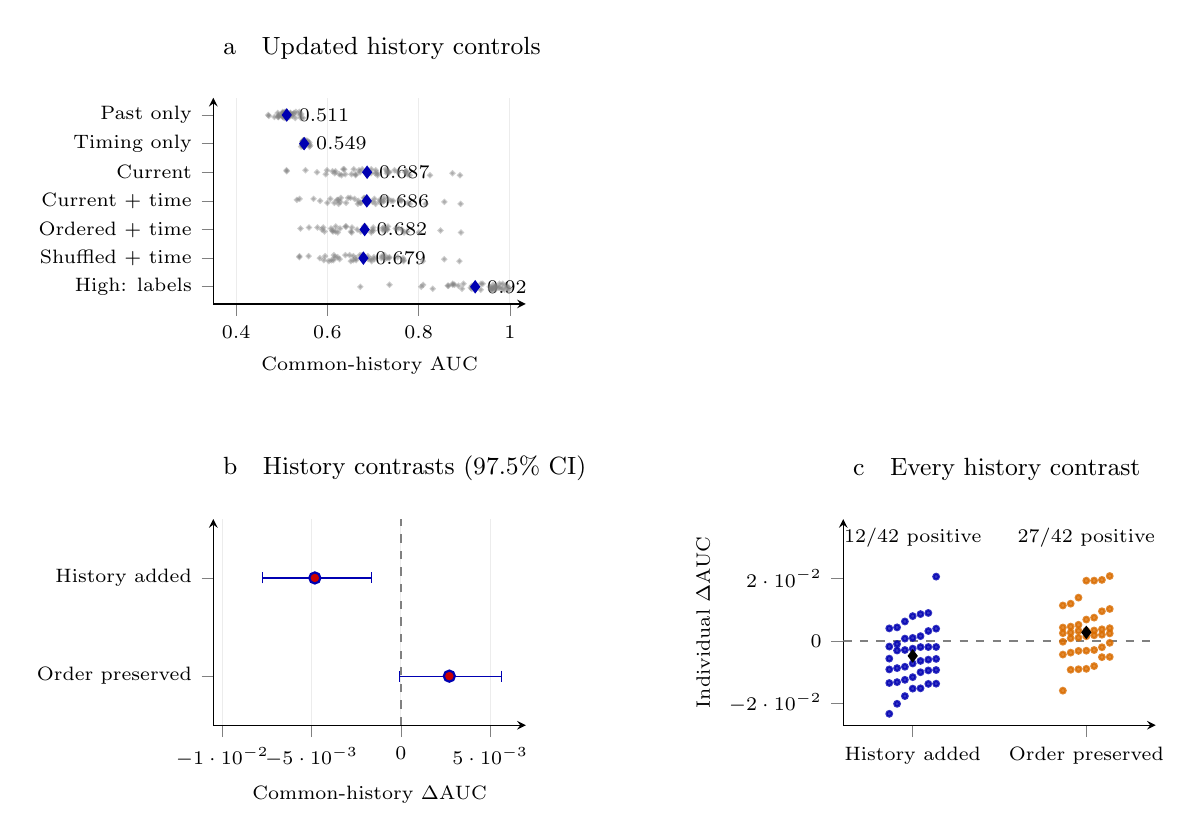
\begin{tikzpicture}
\begin{axis}[axis lines=left,tick align=outside,tick label style={font=\scriptsize},label style={font=\scriptsize},title style={font=\small,align=left},grid style={gray!15},every axis plot/.append style={line width=.8pt},enlarge x limits=false,at={(0cm,0cm)},anchor=north west,width=5.55cm,height=4.2cm,title={a\quad Updated history controls},title style={font=\small,align=left,at={(0,1.06)},anchor=south west},xlabel={Common-history AUC},xmin=.35,xmax=1.035,ymin=-.6,ymax=6.6,ytick={6,5,4,3,2,1,0},yticklabels={Past only,Timing only,Current,Current + time,Ordered + time,Shuffled + time,High: labels},xmajorgrids=true]
\addplot[gray,only marks,mark=*,mark size=.65pt,opacity=.4] coordinates {(0.542295529265,5.895) (0.501880497352,5.93) (0.52305668406,5.965) (0.518295696318,6) (0.500622965501,6.035) (0.502381653956,6.07) (0.509374644724,6.105) (0.505066090027,5.895) (0.491655510518,5.93) (0.506989510514,5.965) (0.518495230892,6) (0.508975575576,6.035) (0.51086651369,6.07) (0.53090813753,6.105) (0.508796922527,5.895) (0.48383885959,5.93) (0.50128189363,5.965) (0.493400277956,6) (0.509666986077,6.035) (0.519133277495,6.07) (0.502049869722,6.105) (0.512026598423,5.895) (0.512175089269,5.93) (0.493525567107,5.965) (0.53893592388,6) (0.505043716504,6.035) (0.526880496771,6.07) (0.508850659612,6.105) (0.546497097018,5.895) (0.516352892676,5.93) (0.514225041226,5.965) (0.470394736842,6) (0.542795365535,6.035) (0.491303937062,6.07) (0.538528926756,6.105) (0.529461402364,5.895) (0.492946526728,5.93) (0.471629363062,5.965) (0.509932836334,6) (0.524675346984,6.035) (0.518381974028,6.07) (0.506596124777,6.105)};
\addplot[gray,only marks,mark=*,mark size=.65pt,opacity=.4] coordinates {(0.54800314615,4.895) (0.545623812363,4.93) (0.548192239961,4.965) (0.548411495976,5) (0.547802451491,5.035) (0.547532151748,5.07) (0.54793702132,5.105) (0.548330290044,4.895) (0.546568121336,4.93) (0.549396407914,4.965) (0.548997338766,5) (0.54923863639,5.035) (0.546128449222,5.07) (0.548361612332,5.105) (0.547178325905,4.895) (0.547402222258,4.93) (0.550030974262,4.965) (0.547301294887,5) (0.546832620655,5.035) (0.547816372508,5.07) (0.547852335135,5.105) (0.547880177168,4.895) (0.548208481147,4.93) (0.545948636088,4.965) (0.546412669981,5) (0.546368266456,5.035) (0.546542187715,5.07) (0.546488508314,5.105) (0.542610708396,4.895) (0.562279914457,4.93) (0.544440102377,4.965) (0.545427803353,5) (0.551444190601,5.035) (0.557508889309,5.07) (0.554989178233,5.105) (0.560546069809,4.895) (0.546034380583,4.93) (0.560445152535,4.965) (0.545548045211,5) (0.560495611172,5.035) (0.545859385736,5.07) (0.551886508864,5.105)};
\addplot[gray,only marks,mark=*,mark size=.65pt,opacity=.4] coordinates {(0.70977232177,3.895) (0.638918986643,3.93) (0.710048421937,3.965) (0.735765180289,4) (0.611065352213,4.035) (0.669387452059,4.07) (0.65789101236,4.105) (0.661886344179,3.895) (0.626209098313,3.93) (0.73085802187,3.965) (0.671447762545,4) (0.77319647427,4.035) (0.705955643,4.07) (0.676429166386,4.105) (0.824980336564,3.895) (0.775372793229,3.93) (0.695475437526,3.965) (0.754732565667,4) (0.771709245643,4.035) (0.7472987427,4.07) (0.636786750904,4.105) (0.630830875887,3.895) (0.59659213509,3.93) (0.874024078719,3.965) (0.734257070136,4) (0.511096605744,4.035) (0.510441717054,4.07) (0.634997251615,4.105) (0.890775302322,3.895) (0.662371598873,3.93) (0.704939363749,3.965) (0.770464734781,4) (0.730653943933,4.035) (0.599210268655,4.07) (0.727654339013,4.105) (0.780397571114,3.895) (0.65283384293,3.93) (0.616127868627,3.965) (0.577347722276,4) (0.617796224406,4.035) (0.552096932115,4.07) (0.696228270579,4.105)};
\addplot[gray,only marks,mark=*,mark size=.65pt,opacity=.4] coordinates {(0.70552177131,2.895) (0.64088417018,2.93) (0.714421941379,2.965) (0.739725709566,3) (0.621415628197,3.035) (0.659547613358,3.07) (0.650640482781,3.105) (0.666883989207,2.895) (0.615301981657,2.93) (0.72118523537,2.965) (0.66769140818,3) (0.758333468677,3.035) (0.703196961506,3.07) (0.679865337364,3.105) (0.815363234131,2.895) (0.776646566265,2.93) (0.691357136725,2.965) (0.744140992058,3) (0.760973821528,3.035) (0.733298840147,3.07) (0.645236808096,3.105) (0.624782194091,2.895) (0.599891416069,2.93) (0.856358308411,2.965) (0.723674777206,3) (0.533064363749,3.035) (0.539005599835,3.07) (0.629717345747,3.105) (0.892012075718,2.895) (0.674056530851,2.93) (0.699182784801,2.965) (0.761910385461,3) (0.714794901745,3.035) (0.606317421327,3.07) (0.723860278961,3.105) (0.780545726261,2.895) (0.672005977738,2.93) (0.628502044112,2.965) (0.58391808094,3) (0.623705252851,3.035) (0.569564209152,3.07) (0.682050467226,3.105)};
\addplot[gray,only marks,mark=*,mark size=.65pt,opacity=.4] coordinates {(0.69619469006,1.895) (0.617540945191,1.93) (0.700939436616,1.965) (0.730591202381,2) (0.607715027506,2.035) (0.653779672067,2.07) (0.641178831702,2.105) (0.6531161036,1.895) (0.612216156268,1.93) (0.7227026262,1.965) (0.665201866344,2) (0.749618912165,2.035) (0.700275868149,2.07) (0.683020767837,2.105) (0.800184685489,1.895) (0.77467442222,1.93) (0.684125168502,1.965) (0.730941547971,2) (0.754969222952,2.035) (0.723268747549,2.07) (0.639554713076,2.105) (0.622814690385,1.895) (0.593478467667,1.93) (0.848072983251,1.965) (0.72799493275,2) (0.540989590491,2.035) (0.55957125189,2.07) (0.618111859283,2.105) (0.892735674042,1.895) (0.673055946819,1.93) (0.697359832348,1.965) (0.762861584444,2) (0.72101312354,2.035) (0.591031675141,2.07) (0.732803267143,2.105) (0.768079222207,1.895) (0.651865466538,1.93) (0.610832932527,1.965) (0.587918269891,2) (0.62761526041,2.035) (0.578142177408,2.07) (0.680105125739,2.105)};
\addplot[gray,only marks,mark=*,mark size=.65pt,opacity=.4] coordinates {(0.696823455985,0.895) (0.613266729002,0.93) (0.702970512966,0.965) (0.730873334988,1) (0.616785033979,1.035) (0.656984754166,1.07) (0.639221536741,1.105) (0.651325396807,0.895) (0.608979519864,0.93) (0.725852024232,0.965) (0.662808843558,1) (0.735773532899,1.035) (0.688938128041,1.07) (0.671118298481,1.105) (0.80943195291,0.895) (0.767848483653,0.93) (0.689256919325,0.965) (0.735316923548,1) (0.754144634724,1.035) (0.719949513112,1.07) (0.648506390907,1.105) (0.603294176607,0.895) (0.592450632594,0.93) (0.856142996684,0.965) (0.718506831739,1) (0.538320221245,1.035) (0.538812783427,1.07) (0.61439939192,1.105) (0.889532087399,0.895) (0.66283238285,0.93) (0.694888432733,0.965) (0.765786897073,1) (0.701741359764,1.035) (0.594794386423,1.07) (0.725361155009,1.105) (0.766604971142,0.895) (0.657066356328,0.93) (0.62676583757,0.965) (0.583348220421,1) (0.622465043974,1.035) (0.558854095094,1.07) (0.676044815858,1.105)};
\addplot[gray,only marks,mark=*,mark size=.65pt,opacity=.4] coordinates {(0.988020965051,-0.105) (0.895288431867,-0.07) (0.968536181883,-0.035) (0.968499059171,0) (0.863745727988,0.035) (0.878469523414,0.07) (0.977385308223,0.105) (0.958545532166,-0.105) (0.958580334708,-0.07) (0.978547713125,-0.035) (0.805528035768,0) (0.887325610263,0.035) (0.922406572576,0.07) (0.940756792876,0.105) (0.997519738842,-0.105) (0.983083644429,-0.07) (0.975447966719,-0.035) (0.968350568326,0) (0.990299371466,0.035) (0.963146428215,0.07) (0.936858908175,0.105) (0.936158216996,-0.105) (0.962218360429,-0.07) (0.960209093672,-0.035) (0.956074551685,0) (0.917043853923,0.035) (0.736034767074,0.07) (0.874692953827,0.105) (0.968163820943,-0.105) (0.916749690807,-0.07) (0.995228974852,-0.035) (0.995870980486,0) (0.969029132884,0.035) (0.874939879071,0.07) (0.984332056479,0.105) (0.962787292153,-0.105) (0.830841177683,-0.07) (0.914250377903,-0.035) (0.672222842518,0) (0.865601810499,0.035) (0.809843943246,0.07) (0.898440720764,0.105)};
\addplot[blue!70!black,only marks,mark=diamond*,mark size=1.8pt] coordinates {(0.510956951188,6) (0.549102433051,5) (0.68705535304,4) (0.686441743808,3) (0.68162533209,2) (0.678909261803,1) (0.923978021742,0)};
\node[anchor=west,font=\scriptsize] at (axis cs:0.515956951188,6) {0.511};
\node[anchor=west,font=\scriptsize] at (axis cs:0.554102433051,5) {0.549};
\node[anchor=west,font=\scriptsize] at (axis cs:0.69205535304,4) {0.687};
\node[anchor=west,font=\scriptsize] at (axis cs:0.691441743808,3) {0.686};
\node[anchor=west,font=\scriptsize] at (axis cs:0.68662533209,2) {0.682};
\node[anchor=west,font=\scriptsize] at (axis cs:0.683909261803,1) {0.679};
\node[anchor=west,font=\scriptsize] at (axis cs:0.928978021742,0) {0.924};
\end{axis}
\begin{axis}[axis lines=left,tick align=outside,tick label style={font=\scriptsize},label style={font=\scriptsize},title style={font=\small,align=left},grid style={gray!15},every axis plot/.append style={line width=.8pt},enlarge x limits=false,at={(0cm,-5.35cm)},anchor=north west,width=5.55cm,height=4.2cm,title={b\quad History contrasts (97.5\% CI)},title style={font=\small,align=left,at={(0,1.06)},anchor=south west},xlabel={Common-history $\Delta$AUC},xmin=-.0105,xmax=.007,ymin=-.5,ymax=1.6,ytick={1,0},yticklabels={History added,Order preserved},scaled x ticks=false,xmajorgrids=true]
\addplot[gray,dashed] coordinates {(0,-0.5) (0,1.6)};
\addplot+[blue!70!black,only marks,mark=*,error bars/.cd,x dir=both,x explicit] coordinates {(-0.00481641171842,1) += (0.00315185186623,0) -= (0.00295436316253,0) (0.0027160702861,0) += (0.00291580480051,0) -= (0.00277275084295,0)};
\end{axis}
\begin{axis}[axis lines=left,tick align=outside,tick label style={font=\scriptsize},label style={font=\scriptsize},title style={font=\small,align=left},grid style={gray!15},every axis plot/.append style={line width=.8pt},enlarge x limits=false,at={(8.0cm,-5.35cm)},anchor=north west,width=5.55cm,height=4.2cm,title={c\quad Every history contrast},title style={font=\small,align=left,at={(0,1.06)},anchor=south west},ylabel={Individual $\Delta$AUC},xmin=-.4,xmax=1.4,ymin=-.027,ymax=.039,xtick={0,1},xticklabels={History added,Order preserved},scaled y ticks=false]
\addplot[gray,dashed] coordinates {(-0.4,0) (1.4,0)};
\addplot[blue!70!black,only marks,mark=*,mark size=1pt,opacity=.8] coordinates {(0.135,-0.00932708125001) (-0.135,-0.0233432249892) (-0.135,-0.0134825047621) (-0.135,-0.0091345071844) (0.135,-0.0137006006919) (0.135,-0.00576794129043) (0.09,-0.00946165107899) (0.09,-0.0137678856064) (-0.09,-0.00308582538869) (0.045,0.00151739083023) (0,-0.00248954183614) (-0.09,-0.00871455651121) (-0.045,-0.00292109335666) (0.09,0.00315543047264) (0.045,-0.0151785486412) (0.045,-0.0019721440454) (0,-0.00723196822296) (-0.09,-0.0131994440874) (0.09,-0.00600459857588) (0.045,-0.010030092598) (-0.135,-0.00568209502022) (0.09,-0.00196750370647) (0.045,-0.00641294840175) (-0.045,-0.00828532516015) (-0.09,0.00432015554416) (0,0.00792522674179) (0.135,0.0205656520544) (0,-0.0116054864642) (-0.045,0.000723598323485) (-0.09,-0.00100058403188) (-0.135,-0.00182295245293) (0,0.000951198983097) (-0.045,0.0062182217947) (0,-0.0152857461866) (0.09,0.00894298818194) (-0.045,-0.0124665040539) (-0.09,-0.0201405111997) (-0.045,-0.0176691115844) (-0.135,0.00400018895149) (0.135,0.00391000755806) (0.045,0.00857796825615) (0.135,-0.00194534148688)};
\addplot[black,only marks,mark=diamond*,mark size=1.8pt] coordinates {(0,-0.00481641171842)};
\addplot[orange!85!black,only marks,mark=*,mark size=1pt,opacity=.8] coordinates {(1.135,-0.000628765925063) (0.865,0.00427421618875) (1.09,-0.00203107634982) (0.865,-0.000282132606966) (0.955,-0.00907000647327) (0.955,-0.0032050820992) (1.09,0.00195729496082) (1.045,0.00179070679322) (1,0.00323663640392) (1,-0.00314939803203) (1.135,0.00239302278638) (0.955,0.0138453792665) (0.865,0.0113377401085) (0.91,0.0119024693564) (0.91,-0.00924726742041) (1,0.00682593856655) (1.135,-0.00513175082308) (0.865,-0.00437537557743) (0.91,0.000824588227924) (1.045,0.00331923443688) (1,-0.00895167783055) (1.09,0.0195205137783) (0.955,0.00102783507307) (1.045,-0.00807001343378) (1.09,0.0094881010109) (0.91,0.00266936924557) (1.135,0.0207584684623) (1.09,0.00371246736292) (0.955,0.00320358664285) (1.135,0.0102235639687) (0.865,0.00247139961523) (1.045,-0.00292531262883) (1,0.0192717637763) (0.91,-0.00376271128212) (1.045,0.00744211213412) (1,0.001474251065) (1.09,-0.00520088978975) (0.865,-0.0159329050433) (0.91,0.00457004947094) (0.955,0.00515021643534) (1.045,0.0192880823141) (1.135,0.00406030988045)};
\addplot[black,only marks,mark=diamond*,mark size=1.8pt] coordinates {(1,0.0027160702861)};
\node[font=\scriptsize] at (axis cs:0,.033) {12/42 positive};
\node[font=\scriptsize] at (axis cs:1,.033) {27/42 positive};
\end{axis}
\end{tikzpicture}
\caption{Complete controls evaluated on the separate common-history events in Lee's 42-person confirmation group. (a) All updated classifiers, including the high-channel reference, use these same legal events. Ordered and shuffled conditions include current features and timing. (b) The original 97.5\% confirmation intervals compare ordered/current/timing with current/timing (history added) and with the five-shuffle mean (order preserved). Neither lower bound exceeds zero. (c) Each contrast includes all 42 individual differences; black diamonds mark the means, and dots are offset for visibility. The original-event and common-history masks differ.}
\label{fig:eeg-lee-history}
\end{figure}

\subsection{A personal-feedback advantage is unconfirmed in the new dataset}
\label{sec:source}

The source experiment uses personal task heads with the same number of newly visible feedback trials for each receiving model. Conditions use the participant's own trials, trials from other participants, or an equal mixture. The design matches recipient-level information counts, but not the total collection cost of a shared label pool. Because this experiment uses personal heads and different visible training sets, comparing its scores with those of the pooled budget classifier does not control for architecture.

The Stieger personal-head experiment matches the amount of feedback received by each model. In the 62-participant cohort, personal feedback achieved future balanced accuracy 61.246\%, other-participant feedback 59.061\%, and a half-personal mixture 60.277\%. Other minus personal feedback was $-2.185$ percentage points (97.5\% interval $[-2.918,-1.483]$); mixed minus personal was $-0.970$ ($[-1.484,-0.468]$). The nested 41-participant cohort showed the same direction. These results support an advantage of personal feedback for the evaluated models and budgets in Stieger.

The fixed test of the Stieger direction in Farabbi did not confirm this advantage. Day 3 balanced accuracy was 52.083\% for frozen models, 53.125\% for personal feedback, 54.375\% for other-participant feedback, and 55.417\% for mixed feedback. Other minus personal was $+1.250$ percentage points, with 97.5\% interval $[-2.083,+4.375]$; mixed minus personal was $+2.292$ ($[-0.833,+4.792]$). These intervals establish neither the direction observed in Stieger nor an advantage in the opposite direction. Personal updating minus frozen performance was $+1.042$ percentage points (95\% interval $[-1.458,+3.333]$).

Classification performance also affects the interpretation of this comparison. The Farabbi frozen score AUC was 0.5667, with interval $[0.5069,0.6183]$, whereas its mean balanced accuracy was near chance. Later training-only regularization selection and score-based evaluation did not establish a strong replacement decoder: the six-setting selection yielded balanced accuracy 51.250\%, AUC 0.505833, and Brier score 0.252480, with all three differences against the constant reference crossing zero. The development diagnostic therefore did not establish a stronger classification starting point through training-only selection. It does not identify the cause of the unconfirmed source advantage or constitute a new confirmation.

\begin{figure}[tbp]
\centering
\begingroup
\definecolor{sourceGray}{HTML}{565D64}
\definecolor{sourceOwn}{HTML}{23698D}
\definecolor{sourceOther}{HTML}{B35145}
\definecolor{sourceMixed}{HTML}{B48121}
\definecolor{sourcePerson}{HTML}{9EA6AF}
\begin{tikzpicture}
\pgfplotsset{sourceaxis/.style={scale only axis,width=6.0cm,height=3.7cm,
axis lines=left,axis line style={line width=.45pt},tick style={line width=.4pt},
font=\fontsize{7.5}{8.5}\selectfont,tick label style={font=\fontsize{7}{8}\selectfont},
label style={font=\fontsize{7.5}{8.5}\selectfont},
ymajorgrids=true,grid style={gray!18,line width=.3pt},
title style={align=left,at={(0,1.035)},anchor=south west,font=\fontsize{8}{9}\selectfont},
clip=false}}
\begin{axis}[sourceaxis,at={(0cm,0cm)},anchor=south west,xmin=-.3,xmax=3.3,ymin=30,ymax=80,xtick={0,1,2,3},xticklabels={Frozen,Own,Other,Mixed},ytick={30,40,50,60,70,80},title={\textbf{A  Stieger: 62 participants}\\{\fontsize{7}{8}\selectfont Sessions 2--7; means and 95\% intervals}},ylabel={Future balanced accuracy (\%)}]
\addplot[gray!65,dashed,line width=.5pt,forget plot] coordinates {(-.3,50) (3.3,50)};
\addplot[sourcePerson,opacity=.5,line width=.32pt,mark=*,mark size=.7pt,forget plot] coordinates {(0,59.4261459283) (1,58.4396302721) (2,58.571180627) (3,61.6087559365)};
\addplot[sourcePerson,opacity=.5,line width=.32pt,mark=*,mark size=.7pt,forget plot] coordinates {(0,58.8047076543) (1,61.6260352612) (2,60.0817953799) (3,56.7061466049)};
\addplot[sourcePerson,opacity=.5,line width=.32pt,mark=*,mark size=.7pt,forget plot] coordinates {(0,70.3727027475) (1,72.8615581334) (2,68.2181122337) (3,71.1227145437)};
\addplot[sourcePerson,opacity=.5,line width=.32pt,mark=*,mark size=.7pt,forget plot] coordinates {(0,52.5105220322) (1,52.8872496404) (2,53.4299911877) (3,51.6657990438)};
\addplot[sourcePerson,opacity=.5,line width=.32pt,mark=*,mark size=.7pt,forget plot] coordinates {(0,59.2853786584) (1,56.8500474126) (2,57.0205661991) (3,59.3704548725)};
\addplot[sourcePerson,opacity=.5,line width=.32pt,mark=*,mark size=.7pt,forget plot] coordinates {(0,57.0281490831) (1,57.1536950396) (2,56.047604226) (3,55.7506216139)};
\addplot[sourcePerson,opacity=.5,line width=.32pt,mark=*,mark size=.7pt,forget plot] coordinates {(0,56.4098550053) (1,55.8095020547) (2,54.8438583756) (3,55.8340087495)};
\addplot[sourcePerson,opacity=.5,line width=.32pt,mark=*,mark size=.7pt,forget plot] coordinates {(0,70.7883974084) (1,73.9946223167) (2,69.1402412906) (3,71.3657923498)};
\addplot[sourcePerson,opacity=.5,line width=.32pt,mark=*,mark size=.7pt,forget plot] coordinates {(0,68.0114748238) (1,69.6356265506) (2,67.46556303) (3,71.3668213385)};
\addplot[sourcePerson,opacity=.5,line width=.32pt,mark=*,mark size=.7pt,forget plot] coordinates {(0,56.2715201598) (1,56.4755720171) (2,53.0547353102) (3,54.8923535915)};
\addplot[sourcePerson,opacity=.5,line width=.32pt,mark=*,mark size=.7pt,forget plot] coordinates {(0,62.3027446978) (1,63.4529092822) (2,58.193133285) (3,63.0422507149)};
\addplot[sourcePerson,opacity=.5,line width=.32pt,mark=*,mark size=.7pt,forget plot] coordinates {(0,59.4379110041) (1,58.0864728612) (2,57.3573781909) (3,58.8845724308)};
\addplot[sourcePerson,opacity=.5,line width=.32pt,mark=*,mark size=.7pt,forget plot] coordinates {(0,59.5500950377) (1,57.3232608859) (2,55.7633494835) (3,55.3357099359)};
\addplot[sourcePerson,opacity=.5,line width=.32pt,mark=*,mark size=.7pt,forget plot] coordinates {(0,60.4095197742) (1,61.3531974135) (2,53.7068202609) (3,56.2532087081)};
\addplot[sourcePerson,opacity=.5,line width=.32pt,mark=*,mark size=.7pt,forget plot] coordinates {(0,56.2627787427) (1,55.0700687625) (2,55.4464353898) (3,53.3338051208)};
\addplot[sourcePerson,opacity=.5,line width=.32pt,mark=*,mark size=.7pt,forget plot] coordinates {(0,60.9991635965) (1,61.5131941439) (2,59.1252910579) (3,63.3267003056)};
\addplot[sourcePerson,opacity=.5,line width=.32pt,mark=*,mark size=.7pt,forget plot] coordinates {(0,63.0630031057) (1,63.5062772167) (2,63.2278067624) (3,60.9822473397)};
\addplot[sourcePerson,opacity=.5,line width=.32pt,mark=*,mark size=.7pt,forget plot] coordinates {(0,50.5252205629) (1,50.5670456249) (2,52.0655111617) (3,51.7914661865)};
\addplot[sourcePerson,opacity=.5,line width=.32pt,mark=*,mark size=.7pt,forget plot] coordinates {(0,53.0942610575) (1,56.2382028719) (2,52.1477363594) (3,56.7091842864)};
\addplot[sourcePerson,opacity=.5,line width=.32pt,mark=*,mark size=.7pt,forget plot] coordinates {(0,70.6590499133) (1,72.2785601672) (2,67.3078657921) (3,71.2636434414)};
\addplot[sourcePerson,opacity=.5,line width=.32pt,mark=*,mark size=.7pt,forget plot] coordinates {(0,59.0835727927) (1,58.6246422827) (2,59.8194878578) (3,58.765831049)};
\addplot[sourcePerson,opacity=.5,line width=.32pt,mark=*,mark size=.7pt,forget plot] coordinates {(0,64.6138896352) (1,66.7749143017) (2,65.9946188742) (3,66.2002972788)};
\addplot[sourcePerson,opacity=.5,line width=.32pt,mark=*,mark size=.7pt,forget plot] coordinates {(0,71.638244381) (1,73.9233224202) (2,70.6572601907) (3,72.7191257192)};
\addplot[sourcePerson,opacity=.5,line width=.32pt,mark=*,mark size=.7pt,forget plot] coordinates {(0,67.0867963466) (1,70.7977698609) (2,66.6716659142) (3,69.9566118679)};
\addplot[sourcePerson,opacity=.5,line width=.32pt,mark=*,mark size=.7pt,forget plot] coordinates {(0,62.4631279512) (1,60.7734884471) (2,62.953930529) (3,60.5363969253)};
\addplot[sourcePerson,opacity=.5,line width=.32pt,mark=*,mark size=.7pt,forget plot] coordinates {(0,61.2473178086) (1,63.6110382514) (2,58.9966328835) (3,62.3709804307)};
\addplot[sourcePerson,opacity=.5,line width=.32pt,mark=*,mark size=.7pt,forget plot] coordinates {(0,69.1318125244) (1,68.5514137171) (2,67.8298894959) (3,69.579418886)};
\addplot[sourcePerson,opacity=.5,line width=.32pt,mark=*,mark size=.7pt,forget plot] coordinates {(0,61.823899992) (1,63.2713263122) (2,62.5277694585) (3,63.5001725523)};
\addplot[sourcePerson,opacity=.5,line width=.32pt,mark=*,mark size=.7pt,forget plot] coordinates {(0,55.5530061694) (1,54.7653695067) (2,53.5550927805) (3,54.325391528)};
\addplot[sourcePerson,opacity=.5,line width=.32pt,mark=*,mark size=.7pt,forget plot] coordinates {(0,57.3104553825) (1,63.9273006029) (2,58.3566616521) (3,60.795834558)};
\addplot[sourcePerson,opacity=.5,line width=.32pt,mark=*,mark size=.7pt,forget plot] coordinates {(0,54.9816868555) (1,54.1375404456) (2,55.6224816518) (3,55.3351406631)};
\addplot[sourcePerson,opacity=.5,line width=.32pt,mark=*,mark size=.7pt,forget plot] coordinates {(0,70.6928691898) (1,71.9325251729) (2,67.3465752687) (3,69.6092084941)};
\addplot[sourcePerson,opacity=.5,line width=.32pt,mark=*,mark size=.7pt,forget plot] coordinates {(0,56.4257788714) (1,57.3781150456) (2,56.0735215074) (3,56.4100338584)};
\addplot[sourcePerson,opacity=.5,line width=.32pt,mark=*,mark size=.7pt,forget plot] coordinates {(0,63.535665484) (1,62.4103683113) (2,59.4378525348) (3,62.4749809926)};
\addplot[sourcePerson,opacity=.5,line width=.32pt,mark=*,mark size=.7pt,forget plot] coordinates {(0,63.9297242637) (1,68.3522301363) (2,59.8074024288) (3,63.2941512384)};
\addplot[sourcePerson,opacity=.5,line width=.32pt,mark=*,mark size=.7pt,forget plot] coordinates {(0,69.398979258) (1,71.0197445258) (2,65.7756041989) (3,69.8390955767)};
\addplot[sourcePerson,opacity=.5,line width=.32pt,mark=*,mark size=.7pt,forget plot] coordinates {(0,58.8724416988) (1,60.5338897815) (2,59.4470339597) (3,59.720042486)};
\addplot[sourcePerson,opacity=.5,line width=.32pt,mark=*,mark size=.7pt,forget plot] coordinates {(0,60.2604467926) (1,59.2807732507) (2,60.0218577898) (3,60.2767895367)};
\addplot[sourcePerson,opacity=.5,line width=.32pt,mark=*,mark size=.7pt,forget plot] coordinates {(0,62.6719260943) (1,62.5029086495) (2,63.0431782989) (3,63.4305725139)};
\addplot[sourcePerson,opacity=.5,line width=.32pt,mark=*,mark size=.7pt,forget plot] coordinates {(0,70.6867706781) (1,69.5767389188) (2,69.3058383585) (3,68.2098682248)};
\addplot[sourcePerson,opacity=.5,line width=.32pt,mark=*,mark size=.7pt,forget plot] coordinates {(0,56.0235912646) (1,53.913611227) (2,55.42448964) (3,54.4042434983)};
\addplot[sourcePerson,opacity=.5,line width=.32pt,mark=*,mark size=.7pt,forget plot] coordinates {(0,63.2580956002) (1,66.8795992565) (2,60.6696658308) (3,61.5405088785)};
\addplot[sourcePerson,opacity=.5,line width=.32pt,mark=*,mark size=.7pt,forget plot] coordinates {(0,69.5351487373) (1,69.3369421651) (2,66.5313004994) (3,68.725751697)};
\addplot[sourcePerson,opacity=.5,line width=.32pt,mark=*,mark size=.7pt,forget plot] coordinates {(0,53.4341041389) (1,55.0059108391) (2,55.8727961814) (3,52.017621804)};
\addplot[sourcePerson,opacity=.5,line width=.32pt,mark=*,mark size=.7pt,forget plot] coordinates {(0,52.7356628468) (1,55.8888013741) (2,54.6556257968) (3,54.1807018449)};
\addplot[sourcePerson,opacity=.5,line width=.32pt,mark=*,mark size=.7pt,forget plot] coordinates {(0,64.7524662257) (1,62.7419155726) (2,59.8421825311) (3,61.478481445)};
\addplot[sourcePerson,opacity=.5,line width=.32pt,mark=*,mark size=.7pt,forget plot] coordinates {(0,56.8806692623) (1,58.2380992373) (2,55.5559186298) (3,57.7282214227)};
\addplot[sourcePerson,opacity=.5,line width=.32pt,mark=*,mark size=.7pt,forget plot] coordinates {(0,58.6453957176) (1,58.5014270425) (2,59.5040949559) (3,57.8190371971)};
\addplot[sourcePerson,opacity=.5,line width=.32pt,mark=*,mark size=.7pt,forget plot] coordinates {(0,50.6083447849) (1,54.4554825085) (2,51.6227071769) (3,53.0509531189)};
\addplot[sourcePerson,opacity=.5,line width=.32pt,mark=*,mark size=.7pt,forget plot] coordinates {(0,62.6652241579) (1,63.7263008635) (2,59.4251178101) (3,61.7680027845)};
\addplot[sourcePerson,opacity=.5,line width=.32pt,mark=*,mark size=.7pt,forget plot] coordinates {(0,59.4940099594) (1,58.0383351577) (2,56.6309190291) (3,57.0216510363)};
\addplot[sourcePerson,opacity=.5,line width=.32pt,mark=*,mark size=.7pt,forget plot] coordinates {(0,62.5008745619) (1,61.6908939473) (2,57.7666535614) (3,61.3356846595)};
\addplot[sourcePerson,opacity=.5,line width=.32pt,mark=*,mark size=.7pt,forget plot] coordinates {(0,59.5636511178) (1,57.0824420781) (2,60.0203391242) (3,60.0248617334)};
\addplot[sourcePerson,opacity=.5,line width=.32pt,mark=*,mark size=.7pt,forget plot] coordinates {(0,51.5020646043) (1,53.0334857841) (2,51.855719812) (3,51.285828287)};
\addplot[sourcePerson,opacity=.5,line width=.32pt,mark=*,mark size=.7pt,forget plot] coordinates {(0,55.1948781174) (1,54.6963409169) (2,54.0591271634) (3,53.0893951325)};
\addplot[sourcePerson,opacity=.5,line width=.32pt,mark=*,mark size=.7pt,forget plot] coordinates {(0,64.1100589855) (1,65.4099728526) (2,58.6566728579) (3,61.2697501733)};
\addplot[sourcePerson,opacity=.5,line width=.32pt,mark=*,mark size=.7pt,forget plot] coordinates {(0,70.1411510802) (1,67.6654119036) (2,65.4303553002) (3,65.9490961905)};
\addplot[sourcePerson,opacity=.5,line width=.32pt,mark=*,mark size=.7pt,forget plot] coordinates {(0,57.4539640481) (1,57.181486043) (2,53.8364824552) (3,54.7358283951)};
\addplot[sourcePerson,opacity=.5,line width=.32pt,mark=*,mark size=.7pt,forget plot] coordinates {(0,63.1109027826) (1,62.3178856615) (2,57.4796173576) (3,61.8026454197)};
\addplot[sourcePerson,opacity=.5,line width=.32pt,mark=*,mark size=.7pt,forget plot] coordinates {(0,57.6139889851) (1,53.8984310617) (2,52.7579272728) (3,54.1430227889)};
\addplot[sourcePerson,opacity=.5,line width=.32pt,mark=*,mark size=.7pt,forget plot] coordinates {(0,52.332569137) (1,54.2095635475) (2,48.4673102827) (3,52.8637522841)};
\addplot[sourcePerson,opacity=.5,line width=.32pt,mark=*,mark size=.7pt,forget plot] coordinates {(0,54.7103210555) (1,56.0895353747) (2,50.2529448078) (3,52.9643387276)};
\addplot+[only marks,mark=diamond*,mark size=2pt,color=sourceGray,line width=1pt,error bars/.cd,y dir=both,y explicit,error bar style={line width=1pt},error mark options={rotate=90,mark size=2.5pt}] coordinates {(0,60.6917443602) += (0,1.43729863376) -= (0,1.38887423669)};
\node[font=\fontsize{7.2}{8}\selectfont,text=sourceGray] at (axis cs:0,77) {60.69};
\addplot+[only marks,mark=diamond*,mark size=2pt,color=sourceOwn,line width=1pt,error bars/.cd,y dir=both,y explicit,error bar style={line width=1pt},error mark options={rotate=90,mark size=2.5pt}] coordinates {(1,61.246290682) += (0,1.53199560621) -= (0,1.4691553959)};
\node[font=\fontsize{7.2}{8}\selectfont,text=sourceOwn] at (axis cs:1,77) {61.25};
\addplot+[only marks,mark=diamond*,mark size=2pt,color=sourceOther,line width=1pt,error bars/.cd,y dir=both,y explicit,error bar style={line width=1pt},error mark options={rotate=90,mark size=2.5pt}] coordinates {(2,59.0609241825) += (0,1.37605454376) -= (0,1.30078335956)};
\node[font=\fontsize{7.2}{8}\selectfont,text=sourceOther] at (axis cs:2,77) {59.06};
\addplot+[only marks,mark=diamond*,mark size=2pt,color=sourceMixed,line width=1pt,error bars/.cd,y dir=both,y explicit,error bar style={line width=1pt},error mark options={rotate=90,mark size=2.5pt}] coordinates {(3,60.2767029034) += (0,1.4968166694) -= (0,1.43785230812)};
\node[font=\fontsize{7.2}{8}\selectfont,text=sourceMixed] at (axis cs:3,77) {60.28};
\end{axis}
\begin{axis}[sourceaxis,at={(0cm,-5.55cm)},anchor=south west,xmin=-.45,xmax=1.5,ymin=-12,ymax=12,xtick={0,1},xticklabels={{Other $-$ Own\\48 / 0 / 14},{Mixed $-$ Own\\44 / 0 / 18}},xticklabel style={align=center,font=\fontsize{7}{8}\selectfont},ytick={-10,-5,0,5,10},xlabel={Participants: lower / equal / higher},title={\textbf{C  Stieger: individual differences}\\{\fontsize{7}{8}\selectfont Individuals and paired mean (97.5\% interval)}},ylabel={Paired difference in future BA (pp)}]
\addplot[gray!70,dashed,line width=.55pt,forget plot] coordinates {(-.45,0) (1.5,0)};
\addplot[only marks,mark=*,mark size=1.35pt,draw=white,line width=.2pt,fill=sourceOther,fill opacity=.72,forget plot] coordinates {(-0.1138,0.131550354963) (-0.0176,-1.54423988126) (-0.184,-4.64344589965) (-0.0878,0.542741547249) (0.0084,0.170518786505) (-0.158,-1.10609081365) (-0.0618,-0.965643679076) (0.0344,-4.8543810261) (-0.132,-2.17006352067) (-0.0358,-3.42083670693) (-0.2022,-5.25977599714) (-0.106,-0.729094670309) (-0.0098,-1.55991140245) (-0.1762,-7.64637715258) (-0.08,0.376366627232) (0.0162,-2.38790308603) (-0.1502,-0.27847045426) (-0.054,1.49846553681) (0.0422,-4.09046651251) (-0.1242,-4.97069437512) (-0.028,1.19484557509) (-0.1944,-0.780295427481) (-0.0982,-3.2660622295) (-0.002,-4.12610394677) (-0.1684,2.18044208183) (-0.0722,-4.61440536789) (0.024,-0.721524221258) (-0.1424,-0.743556853674) (-0.0462,-1.21027672616) (0.05,-5.57063895076) (-0.1164,1.48494120618) (-0.0202,-4.58594990425) (-0.1866,-1.30459353815) (-0.0904,-2.97251577652) (0.0058,-8.54482770745) (-0.1606,-5.24414032691) (-0.0644,-1.08685582173) (0.0318,0.741084539116) (-0.1346,0.540269649465) (-0.0384,-0.270900560318) (-0.2048,1.51087841305) (-0.1086,-6.2099334257) (-0.0124,-2.80564166561) (-0.1788,0.866885342241) (-0.0826,-1.23317557729) (0.0136,-2.89973304146) (-0.1528,-2.68218060749) (-0.0566,1.0026679134) (0.0396,-2.83277533157) (-0.1268,-4.30118305341) (-0.0306,-1.40741612859) (-0.197,-3.92424038588) (-0.1008,2.93789704609) (-0.0046,-1.17776597217) (-0.171,-0.637213753501) (-0.0748,-6.75329999472) (0.0214,-2.23505660342) (-0.145,-3.3450035878) (-0.0488,-4.83826830391) (0.0474,-1.14050378886) (-0.119,-5.74225326476) (-0.0228,-5.83659056693)};
\addplot+[only marks,mark=diamond*,mark size=2pt,color=black!85,line width=1pt,error bars/.cd,y dir=both,y explicit,error bar style={line width=1pt},error mark options={rotate=90,mark size=2.5pt}] coordinates {(0.23,-2.18536649952) += (0,0.702392293614) -= (0,0.732850341144)};
\node[font=\fontsize{7.4}{8}\selectfont] at (axis cs:0,11.1) {-2.19 pp};
\addplot[only marks,mark=*,mark size=1.35pt,draw=white,line width=.2pt,fill=sourceMixed,fill opacity=.72,forget plot] coordinates {(0.8862,3.16912566439) (0.9824,-4.91988865636) (0.816,-1.73884358965) (0.9122,-1.22145059659) (1.0084,2.52040745992) (0.842,-1.40307342572) (0.9382,0.0245066947688) (1.0344,-2.62882996687) (0.868,1.73119478783) (0.9642,-1.58321842562) (0.7978,-0.410658567287) (0.894,0.798099569651) (0.9902,-1.98755094997) (0.8238,-5.09998870539) (0.92,-1.73626364171) (1.0162,1.81350616167) (0.8498,-2.52402987701) (0.946,1.22442056161) (1.0422,0.470981414519) (0.8758,-1.01491672588) (0.972,0.141188766249) (0.8056,-0.574617022875) (0.9018,-1.20419670092) (0.998,-0.841157993052) (0.8316,-0.237091521806) (0.9278,-1.24005782068) (1.024,1.02800516892) (0.8576,0.228846240118) (0.9538,-0.439977978678) (1.05,-3.13146604488) (0.8836,1.19760021753) (0.9798,-2.32331667882) (0.8134,-0.968081187142) (0.9096,0.0646126812495) (1.0058,-5.05807889787) (0.8394,-1.18064894911) (0.9356,-0.81384729543) (1.0318,0.996016285981) (0.8654,0.927663864445) (0.9616,-1.36687069396) (0.7952,0.490632271293) (0.8914,-5.33909037801) (0.9876,-0.611190468099) (0.8212,-2.98828903514) (0.9174,-1.70809952914) (1.0136,-1.26343412764) (0.8472,-0.509877814648) (0.9434,-0.682389845371) (1.0396,-1.40452938957) (0.8732,-1.95829807904) (0.9694,-1.01668412136) (0.803,-0.355209287782) (0.8992,2.94241965532) (0.9954,-1.74765749714) (0.829,-1.60694578442) (0.9252,-4.14022267931) (1.0214,-1.71631571309) (0.855,-2.44565764791) (0.9512,-0.515240241738) (1.0474,0.24459172725) (0.881,-1.34581126343) (0.9772,-3.12519664712)};
\addplot+[only marks,mark=diamond*,mark size=2pt,color=black!85,line width=1pt,error bars/.cd,y dir=both,y explicit,error bar style={line width=1pt},error mark options={rotate=90,mark size=2.5pt}] coordinates {(1.23,-0.969587778557) += (0,0.501654826226) -= (0,0.514603999548)};
\node[font=\fontsize{7.4}{8}\selectfont] at (axis cs:1,11.1) {-0.97 pp};
\end{axis}
\begin{axis}[sourceaxis,at={(7.25cm,0cm)},anchor=south west,xmin=-.3,xmax=3.3,ymin=30,ymax=80,xtick={0,1,2,3},xticklabels={Frozen,Own,Other,Mixed},ytick={30,40,50,60,70,80},title={\textbf{B  Farabbi: 12 participants}\\{\fontsize{7}{8}\selectfont Day 3; means and 95\% intervals}}]
\addplot[gray!65,dashed,line width=.5pt,forget plot] coordinates {(-.3,50) (3.3,50)};
\addplot[sourcePerson,opacity=.5,line width=.32pt,mark=*,mark size=.7pt,forget plot] coordinates {(0,52.5) (1,57.5) (2,60) (3,65)};
\addplot[sourcePerson,opacity=.5,line width=.32pt,mark=*,mark size=.7pt,forget plot] coordinates {(0,42.5) (1,47.5) (2,52.5) (3,50)};
\addplot[sourcePerson,opacity=.5,line width=.32pt,mark=*,mark size=.7pt,forget plot] coordinates {(0,50) (1,57.5) (2,55) (3,52.5)};
\addplot[sourcePerson,opacity=.5,line width=.32pt,mark=*,mark size=.7pt,forget plot] coordinates {(0,55) (1,52.5) (2,57.5) (3,57.5)};
\addplot[sourcePerson,opacity=.5,line width=.32pt,mark=*,mark size=.7pt,forget plot] coordinates {(0,60) (1,60) (2,62.5) (3,52.5)};
\addplot[sourcePerson,opacity=.5,line width=.32pt,mark=*,mark size=.7pt,forget plot] coordinates {(0,40) (1,32.5) (2,35) (3,37.5)};
\addplot[sourcePerson,opacity=.5,line width=.32pt,mark=*,mark size=.7pt,forget plot] coordinates {(0,60) (1,60) (2,60) (3,65)};
\addplot[sourcePerson,opacity=.5,line width=.32pt,mark=*,mark size=.7pt,forget plot] coordinates {(0,52.5) (1,55) (2,60) (3,60)};
\addplot[sourcePerson,opacity=.5,line width=.32pt,mark=*,mark size=.7pt,forget plot] coordinates {(0,60) (1,62.5) (2,60) (3,67.5)};
\addplot[sourcePerson,opacity=.5,line width=.32pt,mark=*,mark size=.7pt,forget plot] coordinates {(0,60) (1,60) (2,50) (3,60)};
\addplot[sourcePerson,opacity=.5,line width=.32pt,mark=*,mark size=.7pt,forget plot] coordinates {(0,40) (1,35) (2,45) (3,40)};
\addplot[sourcePerson,opacity=.5,line width=.32pt,mark=*,mark size=.7pt,forget plot] coordinates {(0,52.5) (1,57.5) (2,55) (3,57.5)};
\addplot+[only marks,mark=diamond*,mark size=2pt,color=sourceGray,line width=1pt,error bars/.cd,y dir=both,y explicit,error bar style={line width=1pt},error mark options={rotate=90,mark size=2.5pt}] coordinates {(0,52.0833333333) += (0,3.95833333333) -= (0,4.375)};
\node[font=\fontsize{7.2}{8}\selectfont,text=sourceGray] at (axis cs:0,77) {52.08};
\addplot+[only marks,mark=diamond*,mark size=2pt,color=sourceOwn,line width=1pt,error bars/.cd,y dir=both,y explicit,error bar style={line width=1pt},error mark options={rotate=90,mark size=2.5pt}] coordinates {(1,53.125) += (0,4.79166666667) -= (0,5.83333333333)};
\node[font=\fontsize{7.2}{8}\selectfont,text=sourceOwn] at (axis cs:1,77) {53.12};
\addplot+[only marks,mark=diamond*,mark size=2pt,color=sourceOther,line width=1pt,error bars/.cd,y dir=both,y explicit,error bar style={line width=1pt},error mark options={rotate=90,mark size=2.5pt}] coordinates {(2,54.375) += (0,3.75) -= (0,4.79166666667)};
\node[font=\fontsize{7.2}{8}\selectfont,text=sourceOther] at (axis cs:2,77) {54.38};
\addplot+[only marks,mark=diamond*,mark size=2pt,color=sourceMixed,line width=1pt,error bars/.cd,y dir=both,y explicit,error bar style={line width=1pt},error mark options={rotate=90,mark size=2.5pt}] coordinates {(3,55.4166666667) += (0,4.79166666667) -= (0,5.41666666667)};
\node[font=\fontsize{7.2}{8}\selectfont,text=sourceMixed] at (axis cs:3,77) {55.42};
\end{axis}
\begin{axis}[sourceaxis,at={(7.25cm,-5.55cm)},anchor=south west,xmin=-.45,xmax=1.5,ymin=-12,ymax=12,xtick={0,1},xticklabels={{Other $-$ Own\\4 / 1 / 7},{Mixed $-$ Own\\2 / 2 / 8}},xticklabel style={align=center,font=\fontsize{7}{8}\selectfont},ytick={-10,-5,0,5,10},xlabel={Participants: lower / equal / higher},title={\textbf{D  Farabbi: individual differences}\\{\fontsize{7}{8}\selectfont Individuals and paired mean (97.5\% interval)}}]
\addplot[gray!70,dashed,line width=.55pt,forget plot] coordinates {(-.45,0) (1.5,0)};
\addplot[only marks,mark=*,mark size=1.35pt,draw=white,line width=.2pt,fill=sourceOther,fill opacity=.72,forget plot] coordinates {(-0.1138,2.5) (-0.0176,5) (-0.184,-2.5) (-0.0878,5) (0.0084,2.5) (-0.158,2.5) (-0.0618,0) (0.0344,5) (-0.132,-2.5) (-0.0358,-10) (-0.2022,10) (-0.106,-2.5)};
\addplot+[only marks,mark=diamond*,mark size=2pt,color=black!85,line width=1pt,error bars/.cd,y dir=both,y explicit,error bar style={line width=1pt},error mark options={rotate=90,mark size=2.5pt}] coordinates {(0.23,1.25) += (0,3.125) -= (0,3.33333333333)};
\node[font=\fontsize{7.4}{8}\selectfont] at (axis cs:0,11.1) {+1.25 pp};
\addplot[only marks,mark=*,mark size=1.35pt,draw=white,line width=.2pt,fill=sourceMixed,fill opacity=.72,forget plot] coordinates {(0.8862,7.5) (0.9824,2.5) (0.816,-5) (0.9122,5) (1.0084,-7.5) (0.842,5) (0.9382,5) (1.0344,5) (0.868,5) (0.9642,0) (0.7978,5) (0.894,0)};
\addplot+[only marks,mark=diamond*,mark size=2pt,color=black!85,line width=1pt,error bars/.cd,y dir=both,y explicit,error bar style={line width=1pt},error mark options={rotate=90,mark size=2.5pt}] coordinates {(1.23,2.29166666667) += (0,2.5) -= (0,3.125)};
\node[font=\fontsize{7.4}{8}\selectfont] at (axis cs:1,11.1) {+2.29 pp};
\end{axis}
\end{tikzpicture}
\endgroup
\caption{Feedback source and absolute future performance under the two frozen source-comparison protocols. (A,B) Each gray line connects one participant across four arms; colored diamonds and numbers show cohort means with the original 95\% conditional participant-bootstrap intervals. Stieger uses each participant's mean over sessions 2--7; Farabbi uses day 3. (C,D) All participant differences for other-minus-own and mixed-minus-own are shown, with the original paired means and 97.5\% intervals in black. Counts below each comparison indicate the numbers of participants with lower, equal, or higher BA; horizontal displacement only separates points. Within each stage, the three feedback arms match the number of labels received by each personal readout: 46--210 accumulated labels in Stieger and 10 labels in Farabbi (mixed: 5 own and 5 other). All 62 and all 12 participants are included in their respective dataset comparisons; the datasets are not pooled. Farabbi day-3 BA has 2.5-point resolution from 40 balanced trials per person. The Farabbi source contrasts retain intervals spanning zero; participant-level counts do not establish a reversed population effect. BA: balanced accuracy; pp: percentage points.}
\label{fig:source}
\end{figure}

\subsection{Extended retention outcomes and training-only diagnostics}
\label{sec:retention-extended}

In Stieger, initial task eligibility requires diagnostic balanced accuracy of at least 0.60. Initial structural eligibility requires MSE below the participant's actual initial-mean predictor. Subsequent task adequacy requires
\begin{equation}
 \BA_{is}\geq\max\{0.60,\BA_{i,\mathrm{diagnostic}}-0.05\}.
\end{equation}
Structural adequacy requires MSE no greater than 1.10 times initial diagnostic MSE and nonnegative skill relative to the actual initial-mean predictor on the evaluated session. Two consecutive inadequate sessions confirm failure; two consecutive adequate sessions confirm recovery. A final unconfirmed run and a participant with no failure remain in the analysis with their respective censoring states. Initial ineligibility is reported separately from a subsequent failure.


Initial eligibility was limited in the Stieger development data. In the 62-participant cohort, 29 met the task criterion, 51 the structural criterion, and 25 both. The corresponding counts in the nested 41 were 19, 31, and 16. A claim about maintaining an initial joint capability applies to these eligible groups, not to every participant in the cohort.

The nested 41-participant cohort had a mean old-test change of $+2.643$ percentage points (95\% conditional interval $[+0.201,+4.993]$), with twelve participants declining and eight declining by at least five points. For all twelve participants with old-test declines, future gains relative to zero new labels were positive. Figure~\ref{fig:retention-heterogeneity} shows the full distribution in the nested cohort. These participants are a subset of the 62-person cohort.

The primary loss threshold remains the predefined five percentage points. The saved sensitivity counts for any loss and for two-, five-, and ten-point losses are reported separately for each fitted protocol in Table~\ref{tab:old-loss-sensitivity}. They describe score losses on the fixed old tests. Differences between thresholds reflect both the distribution of observed losses and the discrete score resolution; they do not establish participant-specific population-risk changes.

The paired old-test records comprised 1,550 trials across all 62 participants. Recomputing initial and final balanced accuracy from the paired predictions reproduced all nineteen declines and all twelve declines of at least five points. Table~\ref{tab:old-test-resolution} reports the complete class counts and single-trial score increments. Table~\ref{tab:old-test-paired-flips} reports the initial and final scores and both directions of prediction change for the predefined severe-decline subset. For participant 5, the class counts were eleven and one; the sole minority-class trial changed from correct to incorrect and contributed 50 points to the total 54.545-point decline. These records quantify changes on the fixed excluded trials; participant-specific population-risk changes require additional evaluation.

% Insert after the old-loss threshold sensitivity paragraph (baseline manuscript line 818).
\begin{table}[htbp]
\centering
\small
\setlength{\tabcolsep}{3pt}
\caption{Permanent-old test size and single-trial balanced-accuracy resolution for all 62 participants in the original Stieger reduced-label shared-model experiment. The initial and final models are evaluated on the same trials. $n_0$ and $n_1$ are the stored class counts, and $N=n_0+n_1$. A single correctness flip in class $c$ changes BA by $50/n_c$ percentage points (pp), with the sign determined by the direction of the flip. Values are rounded to three decimals. The two column groups list participants 1--31 and 32--62; they are not separate cohorts.}
\label{tab:old-test-resolution}
\begin{tabular}{@{}rrrrrr@{\hspace{9pt}}rrrrrr@{}}
\toprule
ID & $n_0$ & $n_1$ & $N$ & $50/n_0$ & $50/n_1$ & ID & $n_0$ & $n_1$ & $N$ & $50/n_0$ & $50/n_1$\\
\midrule
1 & 14 & 16 & 30 & 3.571 & 3.125 & 32 & 8 & 9 & 17 & 6.250 & 5.556\\
2 & 15 & 14 & 29 & 3.333 & 3.571 & 33 & 15 & 16 & 31 & 3.333 & 3.125\\
3 & 17 & 15 & 32 & 2.941 & 3.333 & 34 & 10 & 9 & 19 & 5.000 & 5.556\\
4 & 11 & 14 & 25 & 4.545 & 3.571 & 35 & 13 & 15 & 28 & 3.846 & 3.333\\
5 & 11 & 1 & 12 & 4.545 & 50.000 & 36 & 16 & 10 & 26 & 3.125 & 5.000\\
6 & 17 & 11 & 28 & 2.941 & 4.545 & 37 & 15 & 16 & 31 & 3.333 & 3.125\\
7 & 12 & 12 & 24 & 4.167 & 4.167 & 38 & 17 & 12 & 29 & 2.941 & 4.167\\
8 & 11 & 13 & 24 & 4.545 & 3.846 & 39 & 10 & 8 & 18 & 5.000 & 6.250\\
9 & 11 & 9 & 20 & 4.545 & 5.556 & 40 & 19 & 19 & 38 & 2.632 & 2.632\\
10 & 19 & 16 & 35 & 2.632 & 3.125 & 41 & 10 & 18 & 28 & 5.000 & 2.778\\
11 & 17 & 17 & 34 & 2.941 & 2.941 & 42 & 13 & 15 & 28 & 3.846 & 3.333\\
12 & 13 & 14 & 27 & 3.846 & 3.571 & 43 & 8 & 6 & 14 & 6.250 & 8.333\\
13 & 14 & 10 & 24 & 3.571 & 5.000 & 44 & 10 & 15 & 25 & 5.000 & 3.333\\
14 & 11 & 15 & 26 & 4.545 & 3.333 & 45 & 10 & 8 & 18 & 5.000 & 6.250\\
15 & 13 & 11 & 24 & 3.846 & 4.545 & 46 & 11 & 11 & 22 & 4.545 & 4.545\\
16 & 16 & 16 & 32 & 3.125 & 3.125 & 47 & 15 & 19 & 34 & 3.333 & 2.632\\
17 & 11 & 14 & 25 & 4.545 & 3.571 & 48 & 10 & 9 & 19 & 5.000 & 5.556\\
18 & 11 & 10 & 21 & 4.545 & 5.000 & 49 & 10 & 14 & 24 & 5.000 & 3.571\\
19 & 16 & 9 & 25 & 3.125 & 5.556 & 50 & 15 & 15 & 30 & 3.333 & 3.333\\
20 & 10 & 9 & 19 & 5.000 & 5.556 & 51 & 10 & 10 & 20 & 5.000 & 5.000\\
21 & 14 & 12 & 26 & 3.571 & 4.167 & 52 & 10 & 8 & 18 & 5.000 & 6.250\\
22 & 8 & 8 & 16 & 6.250 & 6.250 & 53 & 12 & 11 & 23 & 4.167 & 4.545\\
23 & 12 & 17 & 29 & 4.167 & 2.941 & 54 & 19 & 19 & 38 & 2.632 & 2.632\\
24 & 15 & 12 & 27 & 3.333 & 4.167 & 55 & 11 & 14 & 25 & 4.545 & 3.571\\
25 & 13 & 14 & 27 & 3.846 & 3.571 & 56 & 12 & 16 & 28 & 4.167 & 3.125\\
26 & 16 & 13 & 29 & 3.125 & 3.846 & 57 & 10 & 6 & 16 & 5.000 & 8.333\\
27 & 16 & 12 & 28 & 3.125 & 4.167 & 58 & 13 & 16 & 29 & 3.846 & 3.125\\
28 & 12 & 10 & 22 & 4.167 & 5.000 & 59 & 8 & 13 & 21 & 6.250 & 3.846\\
29 & 12 & 13 & 25 & 4.167 & 3.846 & 60 & 6 & 2 & 8 & 8.333 & 25.000\\
30 & 10 & 15 & 25 & 5.000 & 3.333 & 61 & 17 & 12 & 29 & 2.941 & 4.167\\
31 & 17 & 15 & 32 & 2.941 & 3.333 & 62 & 8 & 6 & 14 & 6.250 & 8.333\\
\bottomrule
\end{tabular}
\end{table}

\begin{table}[htbp]
\centering
\small
\setlength{\tabcolsep}{3pt}
\caption{Paired prediction changes for the 12 participants with the predefined decline of at least five BA percentage points in the original Stieger reduced-label shared-model experiment. Counts compare the final prediction saved at session 7 with its own initialized prediction on the identical permanent-old trial; no fitting occurs after the terminal session. $C\!\to\!W$ denotes correct to wrong; $W\!\to\!C$ denotes wrong to correct. Initial and final BA are percentages, and $\Delta$ is final minus initial BA in percentage points. All 62 participants remain in the analysis; this table displays the predefined severe-decline subset. Counts are descriptive and do not estimate individual population risk.}
\label{tab:old-test-paired-flips}
\begin{tabular}{@{}rrr rrr rrrr@{}}
\toprule
 & & & \multicolumn{3}{c}{BA} & \multicolumn{2}{c}{Class 0} & \multicolumn{2}{c}{Class 1}\\
\cmidrule(lr){4-6}\cmidrule(lr){7-8}\cmidrule(l){9-10}
ID & $n_0$ & $n_1$ & Initial & Final & $\Delta$ & $C\!\to\!W$ & $W\!\to\!C$ & $C\!\to\!W$ & $W\!\to\!C$\\
\midrule
1 & 14 & 16 & 70.536 & 64.286 & -6.250 & 1 & 1 & 2 & 0\\
5 & 11 & 1 & 81.818 & 27.273 & -54.545 & 2 & 1 & 1 & 0\\
8 & 11 & 13 & 57.343 & 48.951 & -8.392 & 1 & 0 & 2 & 1\\
18 & 11 & 10 & 47.727 & 37.727 & -10.000 & 1 & 1 & 2 & 0\\
21 & 14 & 12 & 65.476 & 53.571 & -11.905 & 3 & 2 & 2 & 0\\
26 & 16 & 13 & 37.981 & 25.721 & -12.260 & 0 & 1 & 4 & 0\\
31 & 17 & 15 & 59.412 & 53.137 & -6.275 & 2 & 1 & 2 & 1\\
33 & 15 & 16 & 67.500 & 48.125 & -19.375 & 3 & 0 & 3 & 0\\
49 & 10 & 14 & 80.714 & 73.571 & -7.143 & 0 & 0 & 3 & 1\\
50 & 15 & 15 & 70.000 & 60.000 & -10.000 & 4 & 0 & 0 & 1\\
55 & 11 & 14 & 68.506 & 57.792 & -10.714 & 0 & 0 & 3 & 0\\
61 & 17 & 12 & 61.520 & 52.696 & -8.824 & 3 & 0 & 1 & 1\\
\bottomrule
\end{tabular}
\end{table}

The combination of reduced labels and early pairs also failed to maintain the joint criterion throughout follow-up. Confirmed joint failure occurred in 15 of the 25 initially eligible participants in the 62-participant cohort and 12 of 16 in the nested cohort. Using all labels with early pairs produced 14/25 and 12/16. Structural-only confirmed failure was reduced by early pairing, from 17/51 to 13/51 and from 14/31 to 8/31, but this structural gain did not establish continued joint adequacy.

The personal-update controls further distinguish future performance from old-test retention. In Stieger 62, unconstrained personal feedback gave future accuracy 61.246\%, mean permanent-old accuracy 59.090\%, and severe harm in 23/62. The constrained line update gave future accuracy 61.657\%, old accuracy 60.106\%, and severe harm in 18/62. Line minus unconstrained future accuracy was $+0.411$ percentage points (95\% interval $[+0.085,+0.721]$), but the severe-harm proportion difference was $-8.065$ points ($[-17.742,+1.613]$). The line update satisfied the future tolerance but did not meet the harm criterion. Replaying only personal initial data under the specified weighting also failed to resolve this trade-off: future accuracy was 55.638\% and severe harm occurred in 26/62.

Optimization over the full coefficient space removed the line update's geometric restriction. In the later Stieger comparison, full-space constrained minus unconstrained personal future accuracy was $+0.070$ percentage points (95\% interval $[-0.040,+0.194]$). The severe-harm proportion difference was $-3.226$ points, with interval $[-8.065,0]$. An upper bound of zero did not satisfy the strictly negative harm criterion. Both Stieger cohorts satisfied the future tolerance but did not meet the dual target. In Farabbi, severe harm occurred in 3/12 with personal updating and 2/12 with either constrained method, again without a strictly negative upper bound establishing reduced harm. Figure~\ref{fig:retention-tradeoffs} displays the future--harm trade-offs in three separate Stieger stages, including the initial-output penalty, feedback-source and replay controls, and coefficient constraints.

\begin{figure}[t]
\centering
\begingroup
\definecolor{ret0}{HTML}{0072B2}
\definecolor{ret1}{HTML}{56B4E9}
\definecolor{ret2}{HTML}{E69F00}
\definecolor{ret3}{HTML}{B6BBC2}
\definecolor{retgreen}{HTML}{009E73}
\definecolor{retred}{HTML}{D55E00}
\begin{tikzpicture}[font=\scriptsize]
\begin{axis}[width=4.75cm,height=6.2cm,at={(0cm,0)},anchor=north west,xmin=-3.5,xmax=0.8,ymin=-27,ymax=25,xtick={-3,-2,-1,0},ytick={-20,-10,0,10,20},xlabel={Future BA difference (pp)},axis lines=left,grid=major,grid style={gray!15},tick label style={font=\scriptsize},label style={font=\scriptsize},title={A\quad Output penalty},title style={at={(0,1.15)},anchor=south west},clip=false,ylabel={Severe-old-harm difference (pp)}]
\node[anchor=south,font=\tiny,align=center] at (rel axis cs:.5,1.02){Stage 2: shared; 25\% labels\\Reference harm: 12/62};
\addplot[gray,thin] coordinates {(-3.5,0)(0.8,0)};
\addplot[gray,thin] coordinates {(0,-27)(0,25)};
\addplot[only marks,mark=diamond*,mark size=2pt,mark options={fill=white,draw=black}] coordinates {(0,0)};
\addplot[only marks,mark=*,mark size=2pt,color=ret1,error bars/.cd,x dir=both,x explicit,y dir=both,y explicit,error bar style={line width=.55pt},error mark options={mark size=2pt,line width=.5pt}] coordinates {(-0.5298206062,0) += (0.2346159313,6.451612903) -= (0.2231839037,6.451612903)};
\node[anchor=east,align=left,font=\scriptsize,text=ret1,xshift=-3pt,yshift=8pt] at (axis cs:-0.5298206062,0){$\lambda=0.1$};
\addplot[only marks,mark=*,mark size=2pt,color=ret0,error bars/.cd,x dir=both,x explicit,y dir=both,y explicit,error bar style={line width=.55pt},error mark options={mark size=2pt,line width=.5pt}] coordinates {(-1.971485588,-8.064516129) += (0.4640143098,9.677419355) -= (0.433423886,9.677419355)};
\node[anchor=west,align=left,font=\scriptsize,text=ret0,xshift=8pt,yshift=-6pt] at (axis cs:-1.971485588,-8.064516129){$\lambda=1$};
\addplot[only marks,mark=*,mark size=2pt,color=ret0,error bars/.cd,x dir=both,x explicit,y dir=both,y explicit,error bar style={line width=.55pt},error mark options={mark size=2pt,line width=.5pt}] coordinates {(-2.415631214,-9.677419355) += (0.5247873741,12.90322581) -= (0.4865389264,12.90322581)};
\node[anchor=east,align=left,font=\scriptsize,text=ret0,xshift=-2pt,yshift=-23pt] at (axis cs:-2.415631214,-9.677419355){$\lambda=10$};
\end{axis}
\begin{axis}[width=5.2cm,height=6.2cm,at={(4.85cm,0)},anchor=north west,xmin=-7.5,xmax=1.8,ymin=-27,ymax=25,xtick={-6,-4,-2,0},ytick={-20,-10,0,10,20},xlabel={Future BA difference (pp)},axis lines=left,grid=major,grid style={gray!15},tick label style={font=\scriptsize},label style={font=\scriptsize},title={B\quad Feedback sources},title style={at={(0,1.15)},anchor=south west},clip=false,yticklabels={,, , ,}]
\node[anchor=south,font=\tiny,align=center] at (rel axis cs:.5,1.02){Stage 3: recipient-matched\\Reference harm: 23/62};
\addplot[gray,thin] coordinates {(-7.5,0)(1.8,0)};
\addplot[gray,thin] coordinates {(0,-27)(0,25)};
\addplot[only marks,mark=diamond*,mark size=2pt,mark options={fill=white,draw=black}] coordinates {(0,0)};
\addplot[only marks,mark=*,mark size=2pt,color=retred,error bars/.cd,x dir=both,x explicit,y dir=both,y explicit,error bar style={line width=.55pt},error mark options={mark size=2pt,line width=.5pt}] coordinates {(-2.1853665,-1.612903226) += (0.7023922936,16.12903226) -= (0.7328503411,14.51612903)};
\node[anchor=west,align=left,font=\scriptsize,text=retred,xshift=2pt,yshift=14pt] at (axis cs:-2.1853665,-1.612903226){Other};
\addplot[only marks,mark=*,mark size=2pt,color=ret2,error bars/.cd,x dir=both,x explicit,y dir=both,y explicit,error bar style={line width=.55pt},error mark options={mark size=2pt,line width=.5pt}] coordinates {(-0.9695877786,-4.838709677) += (0.5016548262,11.29032258) -= (0.5146039995,11.29032258)};
\node[anchor=west,align=left,font=\scriptsize,text=ret2,xshift=1pt,yshift=-32pt] at (axis cs:-0.9695877786,-4.838709677){Mixed};
\addplot[only marks,mark=*,mark size=2pt,color=ret3,error bars/.cd,x dir=both,x explicit,y dir=both,y explicit,error bar style={line width=.55pt},error mark options={mark size=2pt,line width=.5pt}] coordinates {(-5.608449497,4.838709677) += (0.9155025939,14.51612903) -= (0.9138514886,16.12903226)};
\node[anchor=west,align=left,font=\scriptsize,text=ret3,xshift=9pt,yshift=10pt] at (axis cs:-5.608449497,4.838709677){Personal\\replay};
\end{axis}
\begin{axis}[width=4.75cm,height=6.2cm,at={(10.15cm,0)},anchor=north west,xmin=-0.7,xmax=1.05,ymin=-27,ymax=25,xtick={-0.5,0,0.5,1},ytick={-20,-10,0,10,20},xlabel={Future BA difference (pp)},axis lines=left,grid=major,grid style={gray!15},tick label style={font=\scriptsize},label style={font=\scriptsize},title={C\quad Constraints},title style={at={(0,1.15)},anchor=south west},clip=false,yticklabels={,, , ,}]
\node[anchor=south,font=\tiny,align=center] at (rel axis cs:.5,1.02){Stage 4: own-feedback IDs\\Reference harm: 23/62};
\addplot[gray,thin] coordinates {(-0.7,0)(1.05,0)};
\addplot[gray,thin] coordinates {(0,-27)(0,25)};
\addplot[retred,dashed,thin] coordinates {(-.5,-27)(-.5,25)};
\addplot[only marks,mark=diamond*,mark size=2pt,mark options={fill=white,draw=black}] coordinates {(0,0)};
\addplot[only marks,mark=*,mark size=2pt,color=retgreen,error bars/.cd,x dir=both,x explicit,y dir=both,y explicit,error bar style={line width=.55pt},error mark options={mark size=2pt,line width=.5pt}] coordinates {(0.4106511058,-8.064516129) += (0.3175151953,9.677419355) -= (0.3199451457,9.677419355)};
\node[anchor=west,align=left,font=\scriptsize,text=retgreen,xshift=3pt,yshift=-29pt] at (axis cs:0.4106511058,-8.064516129){Line};
\addplot[only marks,mark=*,mark size=2pt,color=ret0,error bars/.cd,x dir=both,x explicit,y dir=both,y explicit,error bar style={line width=.55pt},error mark options={mark size=2pt,line width=.5pt}] coordinates {(0.07043073954,-3.225806452) += (0.1234085841,3.225806452) -= (0.110256879,4.838709677)};
\node[anchor=west,align=left,font=\scriptsize,text=ret0,xshift=4pt,yshift=22pt] at (axis cs:0.07043073954,-3.225806452){Full space};
\node[anchor=north west,font=\tiny,align=left,fill=white,inner sep=1pt] at (rel axis cs:.02,.98){Line + full space:\\both fail dual criterion};
\end{axis}
\end{tikzpicture}
\endgroup
\caption{Future-performance and permanent-old-harm trade-offs across separately fixed experimental stages. All panels use the 62-person cohort and show paired differences from the reference for that stage (open diamond). Severe harm means an individual old-test BA loss of at least five percentage points. (A) Shared-model initial-output penalties at 25\% labels, relative to penalty weight zero. (B) Other-source, equal-mixture, and personal-old-replay arms relative to the personal-feedback head with global old replay; every receiving head has matched new-label counts. (C) Line and full-space training-risk constraints relative to the unconstrained personal update, using identical feedback IDs. Horizontal intervals for Other and Mixed are the original 97.5\% intervals; all other horizontal and all vertical intervals are 95\%. These are marginal, conditional participant-bootstrap intervals, not joint confidence regions. Lower harm and higher future BA are preferred. For the constrained arms, the future lower bound must be at least $-0.5$ pp (vertical dashed line) and the harm upper bound must be strictly below zero. Both constrained arms meet the future tolerance but do not establish harm reduction; the full-space harm upper bound equals zero. Differences across panels do not control for architecture. Training-risk feasibility is separate from the permanently excluded old-test outcomes plotted here.}
\label{fig:retention-tradeoffs}
\end{figure}

Feasibility and optimization checks evaluate the fitted initial-training objective, rather than risk on the permanent old test. Later training-only controls examined held-out folds, matched labels, replay weighting, and parameter-radius restrictions. These analyses evaluate generalization within the initial data while preserving the permanent-test boundary. They do not change the unmet predefined future--harm criterion.

Table~\ref{tab:decisions} summarizes the reported interval boundaries and the predefined confirmation and numerical criteria. A favorable point estimate is distinct from satisfying a decision rule.

\begin{table}[tbp]
\centering\small
\caption{Reported contrast boundaries and predefined confirmation and numerical criteria. The Yang row is a descriptive matched-control comparison on an existing analysis dataset. Each bound comes from the original interval for that contrast; no pooled test is added. BA and harm-proportion contrasts are expressed in percentage points. The two retention rows show both required bounds.}
\label{tab:decisions}
\begin{tabularx}{\linewidth}{@{}p{.28\linewidth} X p{.25\linewidth}@{}}
\toprule
Test & Interpretation or required boundary & Observed boundary and decision\\
\midrule
Yang 51: true minus shuffled target NMSE & Descriptive 95\% interval relative to zero & $[-0.04413,+0.86741]$; advantage unconfirmed\\
Lee 42: ordered history minus current + timing, AUC & Lower 97.5\% bound above zero & $-0.007771$; failed\\
Lee 42: ordered minus shuffled history, AUC & Lower 97.5\% bound above zero & $-0.000057$; failed\\
Farabbi 12: other minus personal BA & Upper 97.5\% bound below zero & $+4.375$; unconfirmed\\
Farabbi 12: mixed minus personal BA & Upper 97.5\% bound below zero & $+4.792$; unconfirmed\\
Stieger 62: constrained line minus personal update & Future lower 95\% bound $\geq-0.5$; severe-harm upper 95\% bound $<0$ & $+0.085$ and $+1.613$; future passed, joint failed\\
Stieger 62: full-space minus personal update & Same two boundaries & $-0.040$ and $0$; future passed, joint failed\\
Finite parameter-measurement study & All four numerical criteria in each condition & $0/8$ conditions passed jointly\\
Final fitted-prior study & All four numerical criteria in each condition & $0/20$ conditions passed jointly\\
\bottomrule
\end{tabularx}
\end{table}

The early Stieger joint experiment combines feedback and pairing controls with mean, bias, ridge, separate-head, and uncoupled classification references. Its first-session development grid is $\lambda\in\{0.03,0.1,0.3\}$ and ridge penalty in $\{0.01,0.1,1,10\}$. The selected penalties are fixed before future evaluation. Source-task replay, initial-pair replay, and initial-adapter penalties are each removed in separate ablations with the remaining loss weights unchanged. These ablations evaluate the specified objective and do not establish a general requirement for replay or parameter penalties.

The later independent ridge pairing comparison uses five fixed within-class shuffles. Stieger future windows are sessions 4--7 and 4--11; Yang uses session 3. Table~\ref{tab:pairingextended} reports all three cohort-level diagnostic contrasts. Mapping-only comparisons do not change any task model. The common high target and participant-specific normalizer remain fixed, so changes in normalized error do not result from redefining the target scale after feedback.

The initial-output penalty produced a further retention trade-off. With the reduced label budget, weight one decreased future balanced accuracy relative to weight zero by 1.971 percentage points in Stieger 62 (95\% interval $[-2.405,-1.507]$) and 2.482 points in the nested 41 ($[-2.920,-2.053]$). Severe permanent-old harm counts changed from 12/62 to 7/62 and from 8/41 to 0/41. Mean old accuracy did not improve, and eight participants in the nested cohort still declined by at least two points. Thus, the absence of severe events at that threshold did not establish the absence of harm, and the penalty reduced the future benefit.

\begin{table}[tbp]
\centering\small
\caption{Sensitivity of observed final old-test loss counts to the reporting threshold, reported descriptively. Any denotes a strictly positive BA loss; the remaining columns count losses of at least 2, 5, or 10 percentage points against each model\textquotesingle s own initialization. The 5-point column remains the predefined primary harm event. Each stage uses its own models, objectives, information budgets, and final update times; rows across stages are not a matched comparison. The 41-person Stieger group is nested. Farabbi old-test BA changes in 5-point steps, so equality of its any/2/5-point counts reflects score granularity. All entries are existing saved counts; no interval or test is added.}
\label{tab:old-loss-sensitivity}
\begin{tabular}{@{}llrrrr@{}}
\toprule
Group & Update & Any & $\geq2$ & $\mathbf{\geq5}$ & $\geq10$\\
\midrule
\multicolumn{6}{l}{\textit{Shared-classifier output-penalty study}}\\
Stieger 62 & Reduced labels, no output penalty & 19/62 & 19/62 & 12/62 & 7/62\\
Stieger 62 & Reduced labels, output penalty 1 & 11/62 & 11/62 & 7/62 & 0/62\\
Stieger 41* & Reduced labels, no output penalty & 12/41 & 11/41 & 8/41 & 3/41\\
Stieger 41* & Reduced labels, output penalty 1 & 8/41 & 8/41 & 0/41 & 0/41\\
\midrule
\multicolumn{6}{l}{\textit{Personal-head constraint study}}\\
Stieger 62 & Personal update & 33/62 & 31/62 & 23/62 & 12/62\\
Stieger 62 & Constrained line & 23/62 & 23/62 & 18/62 & 8/62\\
Stieger 62 & Constrained full space & 30/62 & 28/62 & 21/62 & 11/62\\
Stieger 41* & Personal update & 13/41 & 10/41 & 7/41 & 6/41\\
Stieger 41* & Constrained line & 12/41 & 11/41 & 7/41 & 5/41\\
Stieger 41* & Constrained full space & 11/41 & 9/41 & 7/41 & 6/41\\
\midrule
\multicolumn{6}{l}{\textit{Farabbi source and constraint study}}\\
Farabbi 12 & Personal feedback & 3/12 & 3/12 & 3/12 & 1/12\\
Farabbi 12 & Other-participant feedback & 5/12 & 5/12 & 5/12 & 2/12\\
Farabbi 12 & Mixed feedback & 4/12 & 4/12 & 4/12 & 0/12\\
Farabbi 12 & Constrained line & 2/12 & 2/12 & 2/12 & 1/12\\
Farabbi 12 & Constrained full space & 2/12 & 2/12 & 2/12 & 1/12\\
\bottomrule
\end{tabular}
\end{table}

The later training-only cross-fitting study evaluates two separate snapshots of cumulative feedback, rather than a continuous deployment path. At the session 6 snapshot, initial-risk violations on excluded outer folds occurred in 25/62 for the training-risk line update, 40/62 for the full-space update, and 35/62 when a ball constraint limited full-space displacement to the line-update radius (Table~\ref{tab:trainingretention}). The ball constraint reduced mean outer BCE relative to unconstrained full-space geometry, but did not attain the line update's lower BCE or violation count. All quantities in this table are training-only generalization diagnostics, separate from permanent old-test and future endpoints.

\begin{table}[h]
\centering\small
\caption{Training-only retention diagnostic after the session 6 feedback snapshot in Stieger 62. A risk violation occurs when outer-fold BCE exceeds the corresponding teacher BCE by more than 0.01. Evaluation uses training-data folds rather than permanent old tests.}
\label{tab:trainingretention}
\begin{tabular}{@{}lrrr@{}}
\toprule
Update & Mean outer BCE & Risk violations & Outer BA harm $\geq5$ points\\
\midrule
Training-risk line & 0.784533 & 25/62 & 2/62\\
Training-risk full space & 0.837796 & 40/62 & 7/62\\
Training risk plus ball & 0.812639 & 35/62 & 4/62\\
\bottomrule
\end{tabular}
\end{table}

\begin{table}[h]
\centering\small
\caption{Target NMSE differences between true and shuffled pairs in the independent ridge control.}
\label{tab:pairingextended}
\begin{tabular}{@{}lrrr@{}}
\toprule
Cohort & Difference & Lower 95\% & Upper 95\%\\
\midrule
Stieger 62 & $-0.100050$ & $-0.117736$ & $-0.081173$\\
Stieger 41, nested & $-0.088567$ & $-0.106026$ & $-0.070967$\\
Yang 51 & $+0.272373$ & $-0.044130$ & $+0.867408$\\
\bottomrule
\end{tabular}
\end{table}

The Yang analysis also evaluates a target excluded from the adapter's training objective: eight log band-power ratios from P3/P4/O1/O2, with alpha 8--13\,Hz and beta 13--30\,Hz relative to 1--45\,Hz. Ratios use the physically scaled EEG before per-channel standardization. A ridge readout from true initial high coordinates is frozen and then applied to predicted coordinates. The readout's approximation error is evaluated on true high coordinates. This separates performance on the adaptation loss from performance on a specific external spectral function, without treating that function as neural-state truth.

Lee waveform-feature diagnostics compare the fixed high classifier on true and mapped inputs and inspect class-centroid controls, common channel components, and initial-mean prediction. The confirmation results show a mapping MSE benefit alongside an unconfirmed gain from the frozen to the updated mapped classifier. History comparisons use two predefined 97.5\% decision intervals and include all five shuffled representations. Additional high-channel reference scores are descriptive. They cannot be combined with scores from the original-event protocol because the valid events differ.

\begin{table}[tbp]
\centering\small
\caption{Exploratory future-test diagnostics in the 12 Lee development participants. Entries report the saved means with equal participant weights. Skill is one minus component MSE divided by the corresponding error of that participant\textquotesingle s fixed initial-mean predictor on the same future trials. The shared component represents physically equal voltage across omitted channels, projected in the fixed standardized coordinates; the remainder contains spatial deviations. The teacher is the original frozen full-view classifier. The class-gap ratio is computed within each participant by dividing the mapped target-minus-nontarget mean score gap by the teacher gap, then averaging across participants. These component scores and score ratios are not percentages of AUC explained.}
\label{tab:lee-development-diagnostics}
\begin{tabular}{@{}lrr@{}}
\toprule
Diagnostic & Frozen mapping & True-pair update\\
\midrule
Shared-component skill & 0.8599 & 0.8699\\
Spatial-deviation skill & 0.1776 & 0.2083\\
Mapped--teacher score correlation & 0.2577 & 0.3101\\
Mapped/teacher class-gap ratio & 0.0903 & 0.0972\\
Shared fraction of mean-predictor error & 0.6999 & 0.6999\\
\bottomrule
\end{tabular}
\end{table}

Training-only Farabbi dose and regularization controls, and Stieger held-out-fold retention controls, are subsequent development studies. Their internal held-out scores are not additional permanent-test measurements for selecting a claimed retention solution. In the constrained optimization controls, we retain the initial coefficients, optimizer diagnostics, constraint residuals, and teacher-to-candidate distances. Optimizer termination, numerical feasibility, and the external harm criterion are recorded separately.

\section{Simulation configuration and numerical stopping rules}
\label{app:simulation}

\subsection{Information assumptions and simulation methods}

Theory on observability and intermittent measurements links potential information gains to system assumptions \cite{sinopoli2004,sandberg2008,ahdab2025}; identification from multiple views similarly requires assumptions about those views \cite{yao2024}. The constructed-state studies distinguish the information available to an update from the model component it changes; they do not fit a physiological model to the EEG recordings.

\subsubsection{State-space model and estimators}
\label{sec:simulation}

The time-varying experiments use a four-dimensional state $z_t$, two-dimensional low observation $x_t$, and four-dimensional high observation $h_t$:
\begin{align}
 z_t&=A_tz_{t-1}+w_t, & w_t&\sim\mathcal N(0,0.02I_4),\\
 x_t&=C_tz_t+e_t, & e_t&\sim\mathcal N(0,0.12I_2),\\
 h_t&=z_t+u_t, & u_t&\sim\mathcal N(0,0.04I_4).
\end{align}
The initial state covariance is $I_4$. The changing system is defined by two repeated transition blocks and a low-observation map:
\begin{equation}
 A(a)=\operatorname{diag}\!\left(B(a),B(a)\right),\quad
 B(a)=\begin{bmatrix}0.98&\delta(1+a)\\0&0.98+0.015a\end{bmatrix},\quad
 C(c)=(1+0.4c)\begin{bmatrix}1&0&0&0\\0&0&1&0\end{bmatrix}.
\end{equation}
The hidden coordinates are 2 and 4 in this one-based notation. Coupling $\delta$ equals 0, 0.02, or 0.2 in unobservable, weak, and observable conditions. For each coupling, seven mechanisms represent no change and abrupt or gradual changes to $A$, $C$, or both. Abrupt changes begin at follow-up step 80. Gradual progress is $(t-79)/41$ from steps 80 through 120 and is one thereafter.

Each of the 21 conditions uses 512 complete trajectories, 20 initial dense observations, and 240 follow-up steps. All methods use the same underlying state and observation-noise realizations. Initial baseline parameters are known. The conditional linear Gaussian state updates follow recursive Kalman filtering \cite{kalman1960}. State-only filtering, state-plus-$A$, state-plus-$C$, and joint state-plus-parameter filtering use fixed candidate grids with interacting multiple-model mixing. Initial candidate weight is concentrated on the baseline $(a,c)=(0,0)$. For $K>1$ candidates, the transition at every follow-up step keeps probability 0.99 on the current candidate and allocates 0.01 across the remaining candidates; mixing is followed by propagation, low-observation likelihood updating, and any subsequently released high observation. The change time is not supplied to the learner. A true-parameter filter is a privileged reference.

Full-state MSE averages squared error across the four state coordinates and all 240 follow-up times. Hidden-state MSE averages the two hidden coordinates. The reported scalar MSE therefore differs from the unnormalized squared Euclidean error.

The main budget comparison uses either no new high observations or exactly twelve. The periodic schedule is $10,30,\ldots,230$. The innovation trigger uses the pre-update mixture low-observation Mahalanobis statistic, threshold 9.21034, a minimum gap of five, and forced releases when needed to spend the fixed budget by step 239. A hybrid schedule reserves six observations at steps 10, 50, 90, 130, 170, and 210, with six additional innovation-triggered or forced observations under the same minimum gap and final permissible step. Calendar feasibility determines when an optional release is required to exhaust the budget without conflicting with fixed observations. The early known-model history experiment instead varies the interval between high observations: an interval of twelve supplies twenty high observations in 240 steps, including the final step. This acquisition count differs from the twelve-observation budget in the time-varying comparison.

Rao--Blackwellized particle filtering combines sampling for some variables with an analytically tractable conditional filter for others \cite{doucet2000}. Further experiments compare finite grids with Rao--Blackwellized particle filters under continuous parameter diffusion reflected onto $[0,1]^2$, with standard deviation 0.05 per coordinate and a 0.01 probability of jointly resetting both coordinates to independent uniform draws. These experiments use matched generating priors and the original abrupt mechanisms. Later controls use the same 32 saved observable trajectories per generating mechanism, four algorithm seeds, and up to 4,096 particles. Additional $C$ measurements are counted separately from high-state observations; they are released after the current main estimate. Exact scalar $c$ measurements and noisy observations with distribution $\mathcal N(c,0.1^2)$ are compared at the twelve fixed times $10,30,\ldots,230$. These controls quantify how parameter information and inference settings affect a finite implementation.

In the changing-system experiments, the main estimate at time $t$ is saved after assimilating the current low observation and before releasing a selected high observation or finite-budget parameter measurement at that time. A calibration sample therefore cannot improve the prediction already scored at its own release time. The updated state and parameter posteriors can influence subsequent estimates. Privileged current-known-parameter references instead receive their specified true parameters before prediction. The early history controls assimilate only the observations allowed by their respective information sets.

Simulation comparisons use complete trajectories as the statistical unit, with algorithm seeds averaged within trajectory. Reported trajectory intervals are descriptive normal intervals for paired path means. Parameter scans remain descriptive and are not multiplicity-adjusted confirmations.

\subsection{Known-state controls distinguish information from update location}
\label{sec:mechanisms}

In the early known-model experiment, low-observation history had no effect on hidden-coordinate MSE under the constructed unobservable condition: the high-history, current-low, and full-low-history predictors all had hidden MSE 0.138943 at the twelve-step interval. Under observable coupling, adding full low history to the same high history and current low observation reduced hidden MSE from 0.104737 to 0.100404, a reduction of 0.004333 (95\% interval $[0.004027,0.004639]$). This controlled temporal-information gain applies to the specified system; it does not establish equivalent information in an arbitrary EEG history window.

In the time-varying system, the location of change determined which update improved performance. With observable coupling, abrupt dynamics change, and twelve periodic high observations, full-state MSE was 0.200986 for state-only filtering, 0.074032 for state-plus-$A$, 0.288328 for state-plus-$C$, and 0.077578 for joint updating. Updating $A$ reduced MSE by 0.126954 relative to state-only filtering ($[0.119051,0.134857]$ for the reduction). Updating the unchanged $C$ increased it by 0.087342 ($[0.074861,0.099824]$). For abrupt observation-map change, state-plus-$C$ achieved 0.074816, compared with 1.348840 for state-only filtering and 1.416432 for state-plus-$A$. Additional flexibility therefore did not make all updates equally appropriate.

The unobservable dynamics-change construction provided an exact check of available information: the entire low-observation arrays under abrupt and gradual $A$ changes were identical to their no-change controls, with maximum absolute difference zero. No rule using only those arrays can distinguish these paired cases. This property holds for the specified constructed system and does not identify an unobservable physiological change in the EEG recordings.

With twelve high observations and joint grid filtering, MSE was lowest for the periodic schedule, followed by the hybrid schedule and the original trigger in all 21 conditions. For unobservable abrupt $A$ change, the three means were 0.127039, 0.167646, and 0.274132. The hybrid-minus-periodic difference was $+0.040606$ ($[+0.037615,+0.043598]$); hybrid-minus-trigger was $-0.106486$ ($[-0.117654,-0.095318]$). This ranking is specific to the evaluated schedules, trigger, and changes. A low-innovation trigger cannot resolve a change constructed to be invisible in its low input.

\begin{figure}[t]
\centering
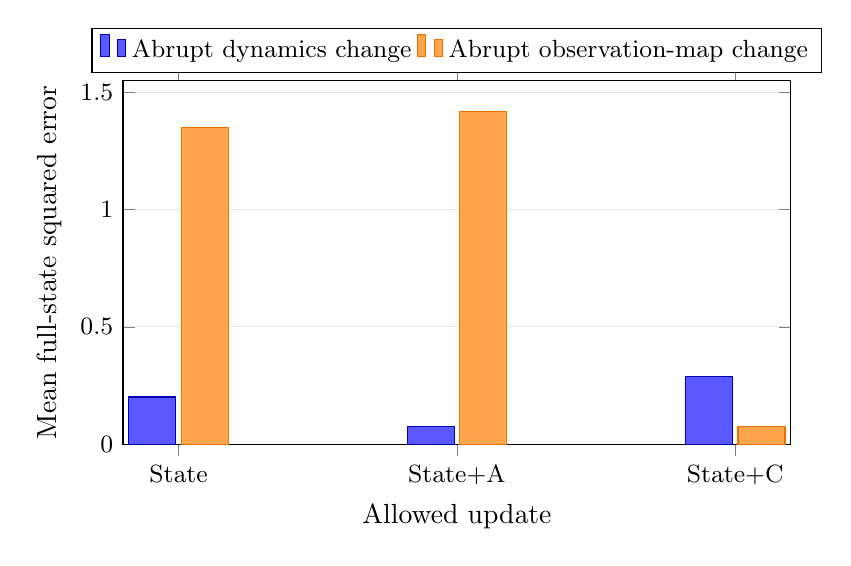
\begin{tikzpicture}
\begin{axis}[width=.83\linewidth,height=62mm,ybar,bar width=17pt,ymin=0,ymax=1.55,ylabel={Mean full-state squared error},symbolic x coords={State,State+A,State+C},xtick=data,xlabel={Allowed update},legend style={at={(.5,1.02)},anchor=south,legend columns=2,font=\small},tick label style={font=\small},ymajorgrids=true,grid style={gray!20}]
\addplot[fill=blue!65,draw=blue!70!black] coordinates {(State,.2009857275)(State+A,.0740316717)(State+C,.2883279330)};
\addplot[fill=orange!70,draw=orange!90!black] coordinates {(State,1.348840)(State+A,1.416432)(State+C,.074816)};
\legend{Abrupt dynamics change,Abrupt observation-map change}
\end{axis}
\end{tikzpicture}
\caption{Update location in a known-state simulation. Each condition has 512 trajectories with observable coupling and twelve periodic high observations. Main estimates are scored before the current high observation is released. Dynamics changes and observation-map changes require different update capabilities. Bars show condition means, not estimates for a population of EEG participants.}
\label{fig:layers}
\end{figure}

The simulations distinguish two reasons for failure of a low-channel update. Failure can arise because the observations lack the necessary information or because the fitted update targets an inappropriate model component. In the constructed unobservable case, some changed and unchanged systems produce identical low observations. Under observable coupling, dynamics and observation-map changes instead favor different update capabilities. Parameter measurements provide another source of information and reduce state error under matched paths. The unresolved particle-stability criteria limit the interpretation of these gains as accurate continuous-parameter inference. These controlled constructions clarify the distinctions evaluated in the EEG experiments without identifying their physiological cause.

The early history experiment uses a known fixed linear-Gaussian model and high-observation intervals 4, 12, and 36. The twelve-step interval and the later twelve-observation schedule involve different acquisition counts. The subsequent changing-system grid uses the fixed progression values $\{0,0.5,1\}$ for each permitted parameter. In the first grid-refinement comparison, expanding to five values also changes the original switching-prior configuration, so this comparison does not isolate a change in computation alone. A subsequent scan holds the continuous physical diffusion and reset prior fixed, while its finite-grid approximations still differ. Under that common physical prior, the finer grid had lower full-state MSE in three of 21 no-high conditions and two of 21 periodic conditions. Figure~\ref{fig:dynamics-history-schedules} separates the early history-information comparison from the later fixed-budget schedule comparison across all 21 conditions.

\begin{figure}[p]
\centering
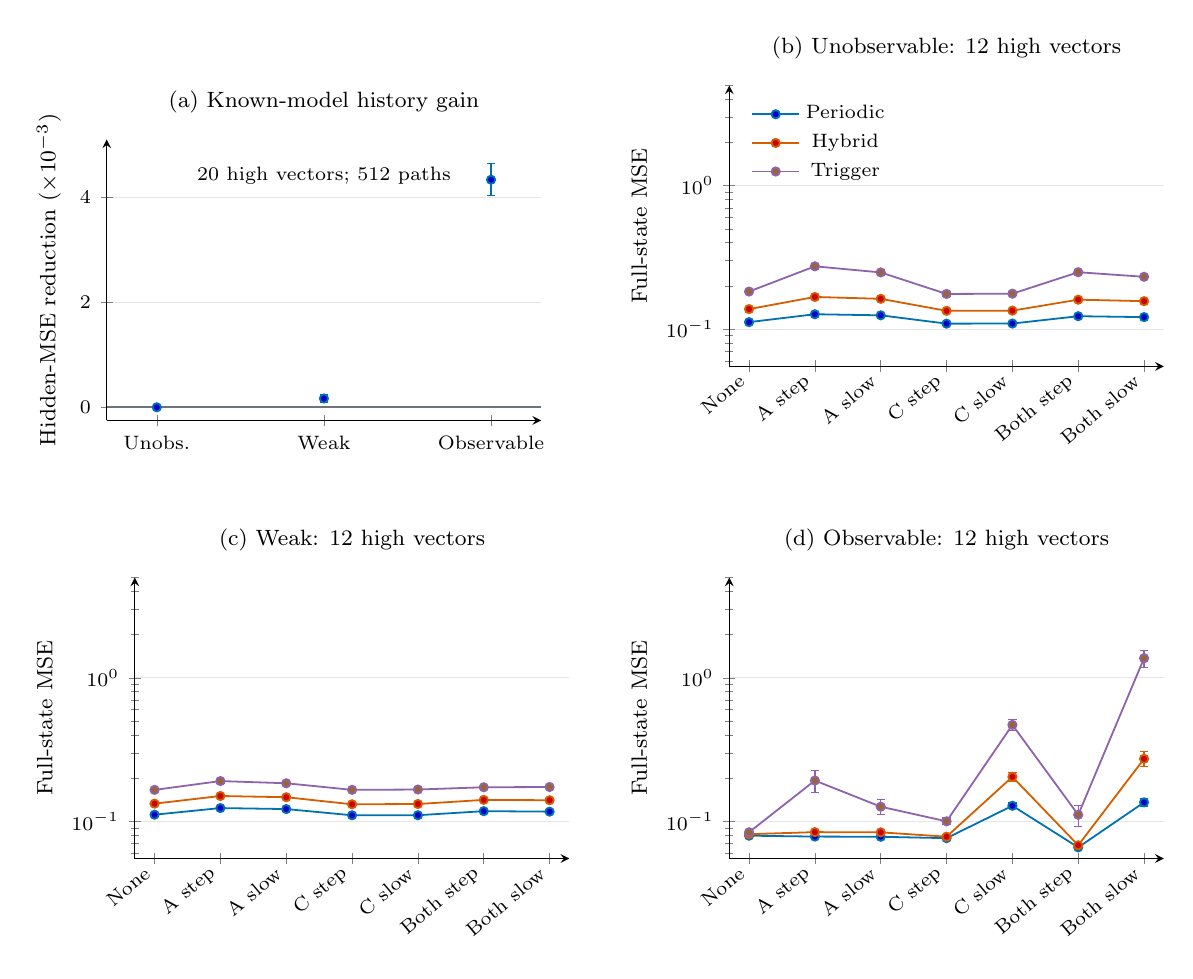
\begin{tikzpicture}
\begin{axis}[at={(0cm,6.25cm)},anchor=outer south west,width=7.1cm,height=5.15cm,font=\fontsize{8}{9.5}\selectfont,tick label style={font=\fontsize{7.5}{9}\selectfont},title style={align=left,font=\fontsize{8.5}{10}\selectfont},title={(a) Known-model history gain},axis x line=bottom,axis y line=left,ymajorgrids=true,grid style={gray!20},legend style={font=\fontsize{7}{8}\selectfont,draw=none,fill=none},xmin=-.3,xmax=2.3,ymin=-.25,ymax=5.1,xtick={0,1,2},xticklabels={Unobs.,Weak,Observable},ylabel={Hidden-MSE reduction ($\times10^{-3}$)}]
\addplot[color={rgb,255:red,109;green,116;blue,123},solid,no marks,forget plot,line width=.7pt] coordinates {(-0.3,0) (2.3,0)};
\addplot+[color={rgb,255:red,0;green,114;blue,178},mark=*,mark size=1.5pt,line width=.65pt,only marks,error bars/.cd,y dir=both,y explicit,error bar style={line width=.45pt}] coordinates {(0,0) += (0,0) -= (0,0) (1,0.167609403779) += (0,0.0680504166762) -= (0,0.0680504166762) (2,4.332730854) += (0,0.306018324936) -= (0,0.306018324936)};
\node[font=\fontsize{7.5}{9}\selectfont] at (rel axis cs:.5,.87) {20 high vectors; 512 paths};
\end{axis}
\begin{axis}[at={(7.55cm,6.25cm)},anchor=outer south west,width=7.1cm,height=5.15cm,font=\fontsize{8}{9.5}\selectfont,tick label style={font=\fontsize{7.5}{9}\selectfont},title style={align=left,font=\fontsize{8.5}{10}\selectfont},title={(b) Unobservable: 12 high vectors},axis x line=bottom,axis y line=left,ymajorgrids=true,grid style={gray!20},legend style={font=\fontsize{7}{8}\selectfont,draw=none,fill=none},ymode=log,ymin=.055,ymax=5,xmin=-.3,xmax=6.3,xtick={0,1,2,3,4,5,6},xticklabels={None,A step,A slow,C step,C slow,Both step,Both slow},x tick label style={rotate=40,anchor=east},ylabel={Full-state MSE},legend pos=north west]
\addplot+[color={rgb,255:red,0;green,114;blue,178},mark=*,mark size=1.5pt,line width=.65pt,solid,error bars/.cd,y dir=both,y explicit,error bar style={line width=.45pt}] coordinates {(0,0.111921820526) += (0,0.00183778888753) -= (0,0.00183778888753) (1,0.127039112192) += (0,0.0022123928096) -= (0,0.0022123928096) (2,0.124836295563) += (0,0.00215912445003) -= (0,0.00215912445003) (3,0.109249076179) += (0,0.00185214290965) -= (0,0.00185214290965) (4,0.10941977076) += (0,0.00185207661076) -= (0,0.00185207661076) (5,0.12308368582) += (0,0.00218205887735) -= (0,0.00218205887735) (6,0.121309182842) += (0,0.00213768705728) -= (0,0.00213768705728)};
\addlegendentry{Periodic}
\addplot+[color={rgb,255:red,213;green,94;blue,0},mark=*,mark size=1.5pt,line width=.65pt,solid,error bars/.cd,y dir=both,y explicit,error bar style={line width=.45pt}] coordinates {(0,0.137938855433) += (0,0.00297928948216) -= (0,0.00297928948216) (1,0.167645611254) += (0,0.00411086320026) -= (0,0.00411086320026) (2,0.162730114228) += (0,0.00392683144493) -= (0,0.00392683144493) (3,0.134171305679) += (0,0.00295100210321) -= (0,0.00295100210321) (4,0.134585490327) += (0,0.0029511211513) -= (0,0.0029511211513) (5,0.160504268988) += (0,0.00390518252333) -= (0,0.00390518252333) (6,0.156675047483) += (0,0.00374103933993) -= (0,0.00374103933993)};
\addlegendentry{Hybrid}
\addplot+[color={rgb,255:red,142;green,99;blue,172},mark=*,mark size=1.5pt,line width=.65pt,solid,error bars/.cd,y dir=both,y explicit,error bar style={line width=.45pt}] coordinates {(0,0.182883538194) += (0,0.00611626201807) -= (0,0.00611626201807) (1,0.274131561656) += (0,0.0132750271617) -= (0,0.0132750271617) (2,0.248562458274) += (0,0.0110057257246) -= (0,0.0110057257246) (3,0.175911449286) += (0,0.00602917716844) -= (0,0.00602917716844) (4,0.176673656016) += (0,0.00606718270445) -= (0,0.00606718270445) (5,0.249363122347) += (0,0.0120292007204) -= (0,0.0120292007204) (6,0.231724010653) += (0,0.0101822809109) -= (0,0.0101822809109)};
\addlegendentry{Trigger}
\end{axis}
\begin{axis}[at={(0cm,0cm)},anchor=outer south west,width=7.1cm,height=5.15cm,font=\fontsize{8}{9.5}\selectfont,tick label style={font=\fontsize{7.5}{9}\selectfont},title style={align=left,font=\fontsize{8.5}{10}\selectfont},title={(c) Weak: 12 high vectors},axis x line=bottom,axis y line=left,ymajorgrids=true,grid style={gray!20},legend style={font=\fontsize{7}{8}\selectfont,draw=none,fill=none},ymode=log,ymin=.055,ymax=5,xmin=-.3,xmax=6.3,xtick={0,1,2,3,4,5,6},xticklabels={None,A step,A slow,C step,C slow,Both step,Both slow},x tick label style={rotate=40,anchor=east},ylabel={Full-state MSE},legend pos=north west]
\addplot+[color={rgb,255:red,0;green,114;blue,178},mark=*,mark size=1.5pt,line width=.65pt,solid,error bars/.cd,y dir=both,y explicit,error bar style={line width=.45pt}] coordinates {(0,0.111148254537) += (0,0.00177080103371) -= (0,0.00177080103371) (1,0.123606155249) += (0,0.00211769609442) -= (0,0.00211769609442) (2,0.121656472259) += (0,0.00206182757982) -= (0,0.00206182757982) (3,0.110098998841) += (0,0.0017835889382) -= (0,0.0017835889382) (4,0.110185029522) += (0,0.00178244821691) -= (0,0.00178244821691) (5,0.117617463515) += (0,0.00200140927676) -= (0,0.00200140927676) (6,0.116709215865) += (0,0.00196860621133) -= (0,0.00196860621133)};
\addplot+[color={rgb,255:red,213;green,94;blue,0},mark=*,mark size=1.5pt,line width=.65pt,solid,error bars/.cd,y dir=both,y explicit,error bar style={line width=.45pt}] coordinates {(0,0.132705771415) += (0,0.00284775159955) -= (0,0.00284775159955) (1,0.150050142217) += (0,0.00344412054668) -= (0,0.00344412054668) (2,0.14712123494) += (0,0.00332726115687) -= (0,0.00332726115687) (3,0.131346749933) += (0,0.00284779010285) -= (0,0.00284779010285) (4,0.131923189571) += (0,0.002878906239) -= (0,0.002878906239) (5,0.140938649547) += (0,0.00316411358) -= (0,0.00316411358) (6,0.14018376449) += (0,0.00312872389395) -= (0,0.00312872389395)};
\addplot+[color={rgb,255:red,142;green,99;blue,172},mark=*,mark size=1.5pt,line width=.65pt,solid,error bars/.cd,y dir=both,y explicit,error bar style={line width=.45pt}] coordinates {(0,0.165488711884) += (0,0.00488602784035) -= (0,0.00488602784035) (1,0.190724636573) += (0,0.00618629379729) -= (0,0.00618629379729) (2,0.18405960079) += (0,0.00579614989275) -= (0,0.00579614989275) (3,0.16561991267) += (0,0.00476902424311) -= (0,0.00476902424311) (4,0.166430396888) += (0,0.00488604632639) -= (0,0.00488604632639) (5,0.172614605239) += (0,0.00480035348062) -= (0,0.00480035348062) (6,0.173319855975) += (0,0.0049580912197) -= (0,0.0049580912197)};
\end{axis}
\begin{axis}[at={(7.55cm,0cm)},anchor=outer south west,width=7.1cm,height=5.15cm,font=\fontsize{8}{9.5}\selectfont,tick label style={font=\fontsize{7.5}{9}\selectfont},title style={align=left,font=\fontsize{8.5}{10}\selectfont},title={(d) Observable: 12 high vectors},axis x line=bottom,axis y line=left,ymajorgrids=true,grid style={gray!20},legend style={font=\fontsize{7}{8}\selectfont,draw=none,fill=none},ymode=log,ymin=.055,ymax=5,xmin=-.3,xmax=6.3,xtick={0,1,2,3,4,5,6},xticklabels={None,A step,A slow,C step,C slow,Both step,Both slow},x tick label style={rotate=40,anchor=east},ylabel={Full-state MSE},legend pos=north west]
\addplot+[color={rgb,255:red,0;green,114;blue,178},mark=*,mark size=1.5pt,line width=.65pt,solid,error bars/.cd,y dir=both,y explicit,error bar style={line width=.45pt}] coordinates {(0,0.0793680579857) += (0,0.000918437653456) -= (0,0.000918437653456) (1,0.0782394549221) += (0,0.0012058691832) -= (0,0.0012058691832) (2,0.0779920890865) += (0,0.00105532385136) -= (0,0.00105532385136) (3,0.0762505763332) += (0,0.00102184041767) -= (0,0.00102184041767) (4,0.128273844896) += (0,0.00582626945187) -= (0,0.00582626945187) (5,0.065783617987) += (0,0.000817931887304) -= (0,0.000817931887304) (6,0.135483208359) += (0,0.00826722315149) -= (0,0.00826722315149)};
\addplot+[color={rgb,255:red,213;green,94;blue,0},mark=*,mark size=1.5pt,line width=.65pt,solid,error bars/.cd,y dir=both,y explicit,error bar style={line width=.45pt}] coordinates {(0,0.0812692903438) += (0,0.00117847567291) -= (0,0.00117847567291) (1,0.0840202648001) += (0,0.0033048588736) -= (0,0.0033048588736) (2,0.0837343601902) += (0,0.00224339669838) -= (0,0.00224339669838) (3,0.0780818089355) += (0,0.00126233383612) -= (0,0.00126233383612) (4,0.204160202281) += (0,0.0153845276122) -= (0,0.0153845276122) (5,0.0680232243966) += (0,0.00158662139119) -= (0,0.00158662139119) (6,0.272535038597) += (0,0.0317857299845) -= (0,0.0317857299845)};
\addplot+[color={rgb,255:red,142;green,99;blue,172},mark=*,mark size=1.5pt,line width=.65pt,solid,error bars/.cd,y dir=both,y explicit,error bar style={line width=.45pt}] coordinates {(0,0.0838173316969) += (0,0.00150597884905) -= (0,0.00150597884905) (1,0.192322401516) += (0,0.0346227480129) -= (0,0.0346227480129) (2,0.126378671392) += (0,0.0156564697759) -= (0,0.0156564697759) (3,0.0998990821877) += (0,0.00552393503905) -= (0,0.00552393503905) (4,0.469731142852) += (0,0.0417096651771) -= (0,0.0417096651771) (5,0.11090083062) += (0,0.0183457277476) -= (0,0.0183457277476) (6,1.37062203452) += (0,0.190739608309) -= (0,0.190739608309)};
\end{axis}
\end{tikzpicture}
\caption{History and acquisition schedules address different questions. (a) Hidden-coordinate MSE with only the current low observation minus MSE with the complete low history, conditional on the same high history, in the known-model experiment (512 trajectories; high observations every 12 steps, giving 20 follow-up vectors). (b--d) The schedule comparison includes all 21 changing-system conditions with the joint $3\times3$ candidate filter, with 512 trajectories per condition and exactly 12 follow-up high vectors for each policy. Periodic releases occur at 10,30,...,230; the hybrid uses six fixed releases plus six causal or budget-forced releases; the trigger also uses forced releases to exhaust its budget. Step and slow denote abrupt and gradual changes. Bars show the stored descriptive 95\% trajectory intervals; the history interval is paired. State estimates precede the current high release. Dense initialization is separate from these follow-up budgets; panels (b--d) use logarithmic MSE axes.}
\label{fig:dynamics-history-schedules}
\end{figure}

A local exact-mixture check compares explicit short-horizon branch enumeration with moment-matched interaction from the same fixed starting trajectories. Among 126 three-step comparisons, exact-mixture realized state MSE was lower in 45 and higher in 81. This local result distinguishes approximation of a likelihood or posterior from its effect on each realized error; it does not supply an exact posterior for the whole 240-step follow-up.

The subsequent matched-prior generation uses the same reflected diffusion and reset mechanism as the continuous fitted prior. The original abrupt paths represent a separate mechanism. Later finite-parameter-information and fitted-prior studies reuse 32 saved paths for each observable mechanism and four algorithm seeds. State paths, low observations, high observations, and initial posteriors remain paired across those interventions. Each path contributes one seed-averaged endpoint to descriptive intervals. The time steps and four seeds do not increase the number of independent paths.

When a privileged reference receives the exact current value of a parameter coordinate, the unknown coordinate follows the reset prior conditional on the supplied value. For reset probability $q=0.01$, supplied coordinate $v_t$, and reflected-diffusion density $f_{\mathrm{reflected}}$, the conditional reset probability is
\begin{equation}
 \frac{q}{q+(1-q)f_{\mathrm{reflected}}(v_t\mid v_{t-1})}.
\end{equation}
Conditioning on this value changes both the proposal and the known observation or dynamics matrix. The same fitted conditional rule is used for deterministic-change paths, for which it is not the true generating posterior.

The final prior scan changes the baseline diffusion standard deviation 0.05 to 0.025 or 0.10, or the baseline joint-reset probability 0.01 to 0.005 or 0.02. The four numerical criteria compare 2,048 with 4,096 particles: absolute mean-MSE change divided by true-parameter reference MSE no greater than 0.01; mean squared state-estimate change divided by that reference no greater than 0.01; the larger of the two parameter-coordinate mean squared changes no greater than $10^{-4}$; and four-seed state-estimate variance at 4,096 particles divided by reference MSE no greater than 0.01. The criteria passed in 5/20, 4/20, 0/20, and 7/20 cells, respectively. No cell passed all four. Figure~\ref{fig:dynamics-prior-stability} shows the paired prior effects and each numerical criterion separately. The protocol stops at 4,096 particles, without selecting additional counts after examining the outcomes.

\begin{table}[h]
\centering\small
\caption{Prior control using the same paths: state MSE at 4,096 particles, averaged over four seeds within each of 32 paths. The first two rows use a matched generating mechanism; the final two use abrupt changes.}
\label{tab:priors}
\begin{tabular}{@{}llrrrrr@{}}
\toprule
Mechanism & High observations & Baseline & $\sigma/2$ & $2\sigma$ & $q/2$ & $2q$\\
\midrule
Matched & None & .337423 & .337665 & .459594 & .330161 & .329937\\
Matched & Periodic 12 & .136503 & .149275 & .149805 & .136414 & .136262\\
Abrupt & None & .347017 & .429282 & .289624 & .360677 & .352857\\
Abrupt & Periodic 12 & .127192 & .098319 & .153625 & .127329 & .128090\\
\bottomrule
\end{tabular}
\end{table}

\begin{figure}[p]
\centering
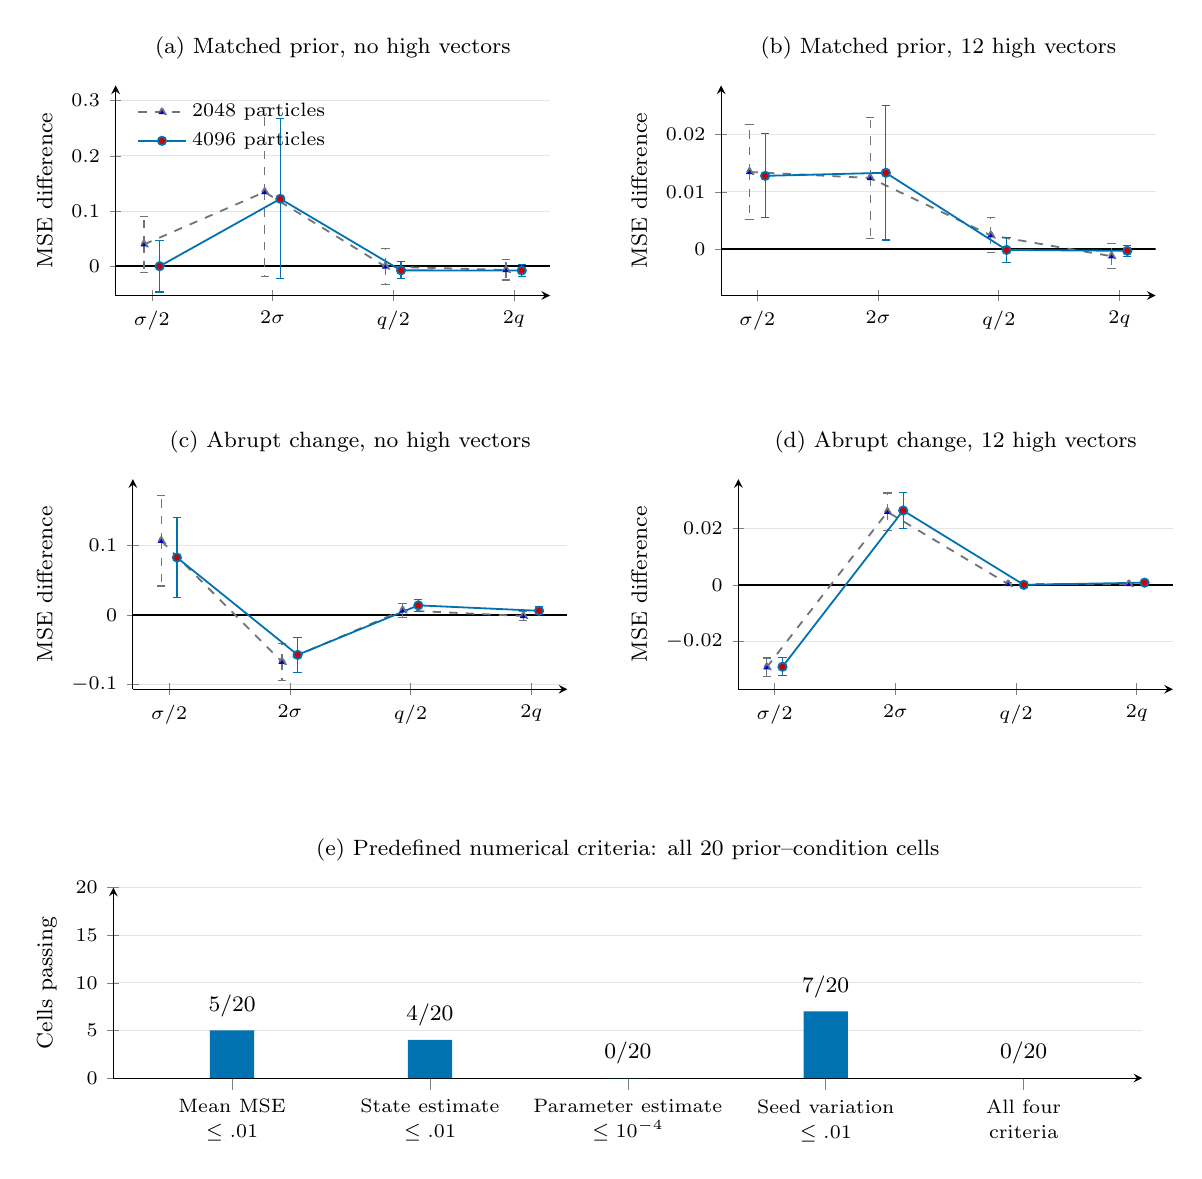
\begin{tikzpicture}
\begin{axis}[at={(0.0cm,10.3cm)},anchor=outer south west,width=7.1cm,height=4.25cm,font=\fontsize{8}{9.5}\selectfont,tick label style={font=\fontsize{7.5}{9}\selectfont},title style={align=left,font=\fontsize{8.5}{10}\selectfont},title={(a) Matched prior, no high vectors},axis x line=bottom,axis y line=left,ymajorgrids=true,grid style={gray!20},legend style={font=\fontsize{7}{8}\selectfont,draw=none,fill=none},xmin=-.3,xmax=3.3,ymin=-0.05279692374777496,ymax=0.3273217037157826,xtick={0,1,2,3},xticklabels={$\sigma/2$,$2\sigma$,$q/2$,$2q$},ylabel={MSE difference},legend pos=north west,scaled y ticks=false,y tick label style={/pgf/number format/fixed,/pgf/number format/precision=3}]
\addplot[color={rgb,255:red,0;green,0;blue,0},solid,no marks,forget plot,line width=.7pt] coordinates {(-0.3,0) (3.3,0)};
\addplot+[color={rgb,255:red,109;green,116;blue,123},mark=triangle*,mark size=1.5pt,line width=.65pt,dashed,error bars/.cd,y dir=both,y explicit,error bar style={line width=.45pt}] coordinates {(-0.065,0.0396734384974) += (0,0.0507479578215) -= (0,0.0507479578215) (0.935,0.134478684045) += (0,0.15264561746) -= (0,0.15264561746) (1.935,-0.000467472933968) += (0,0.0322236640713) -= (0,0.0322236640713) (2.935,-0.00656771223841) += (0,0.0182139771026) -= (0,0.0182139771026)};
\addlegendentry{2048 particles}
\addplot+[color={rgb,255:red,0;green,114;blue,178},mark=*,mark size=1.5pt,line width=.65pt,solid,error bars/.cd,y dir=both,y explicit,error bar style={line width=.45pt}] coordinates {(0.065,0.000241923785928) += (0,0.0465550147927) -= (0,0.0465550147927) (1.065,0.122170716114) += (0,0.144952321475) -= (0,0.144952321475) (2.065,-0.00726262149767) += (0,0.0152657551781) -= (0,0.0152657551781) (3.065,-0.00748604498928) += (0,0.0105127675038) -= (0,0.0105127675038)};
\addlegendentry{4096 particles}
\end{axis}
\begin{axis}[at={(7.55cm,10.3cm)},anchor=outer south west,width=7.1cm,height=4.25cm,font=\fontsize{8}{9.5}\selectfont,tick label style={font=\fontsize{7.5}{9}\selectfont},title style={align=left,font=\fontsize{8.5}{10}\selectfont},title={(b) Matched prior, 12 high vectors},axis x line=bottom,axis y line=left,ymajorgrids=true,grid style={gray!20},legend style={font=\fontsize{7}{8}\selectfont,draw=none,fill=none},xmin=-.3,xmax=3.3,ymin=-0.008,ymax=0.02846921962394228,xtick={0,1,2,3},xticklabels={$\sigma/2$,$2\sigma$,$q/2$,$2q$},ylabel={MSE difference},legend pos=north west,scaled y ticks=false,y tick label style={/pgf/number format/fixed,/pgf/number format/precision=3}]
\addplot[color={rgb,255:red,0;green,0;blue,0},solid,no marks,forget plot,line width=.7pt] coordinates {(-0.3,0) (3.3,0)};
\addplot+[color={rgb,255:red,109;green,116;blue,123},mark=triangle*,mark size=1.5pt,line width=.65pt,dashed,error bars/.cd,y dir=both,y explicit,error bar style={line width=.45pt}] coordinates {(-0.065,0.0134455922793) += (0,0.00818876785496) -= (0,0.00818876785496) (0.935,0.0124006810202) += (0,0.0105233639367) -= (0,0.0105233639367) (1.935,0.00244142501268) += (0,0.00302655001837) -= (0,0.00302655001837) (2.935,-0.00117461981264) += (0,0.00214450094883) -= (0,0.00214450094883)};
\addplot+[color={rgb,255:red,0;green,114;blue,178},mark=*,mark size=1.5pt,line width=.65pt,solid,error bars/.cd,y dir=both,y explicit,error bar style={line width=.45pt}] coordinates {(0.065,0.0127720830125) += (0,0.00730464076982) -= (0,0.00730464076982) (1.065,0.0133024634453) += (0,0.0116705362248) -= (0,0.0116705362248) (2.065,-8.87051234036e-05) += (0,0.00211987124003) -= (0,0.00211987124003) (3.065,-0.000240877955153) += (0,0.000980541524051) -= (0,0.000980541524051)};
\end{axis}
\begin{axis}[at={(0.0cm,5.3cm)},anchor=outer south west,width=7.1cm,height=4.25cm,font=\fontsize{8}{9.5}\selectfont,tick label style={font=\fontsize{7.5}{9}\selectfont},title style={align=left,font=\fontsize{8.5}{10}\selectfont},title={(c) Abrupt change, no high vectors},axis x line=bottom,axis y line=left,ymajorgrids=true,grid style={gray!20},legend style={font=\fontsize{7}{8}\selectfont,draw=none,fill=none},xmin=-.3,xmax=3.3,ymin=-0.10666898155478284,ymax=0.19474988487370345,xtick={0,1,2,3},xticklabels={$\sigma/2$,$2\sigma$,$q/2$,$2q$},ylabel={MSE difference},legend pos=north west,scaled y ticks=false,y tick label style={/pgf/number format/fixed,/pgf/number format/precision=3}]
\addplot[color={rgb,255:red,0;green,0;blue,0},solid,no marks,forget plot,line width=.7pt] coordinates {(-0.3,0) (3.3,0)};
\addplot+[color={rgb,255:red,109;green,116;blue,123},mark=triangle*,mark size=1.5pt,line width=.65pt,dashed,error bars/.cd,y dir=both,y explicit,error bar style={line width=.45pt}] coordinates {(-0.065,0.106106470198) += (0,0.0647267621474) -= (0,0.0647267621474) (0.935,-0.0673768960726) += (0,0.026192385993) -= (0,0.026192385993) (1.935,0.00644693862059) += (0,0.00969633974827) -= (0,0.00969633974827) (2.935,-0.00159426168325) += (0,0.00590827440938) -= (0,0.00590827440938)};
\addplot+[color={rgb,255:red,0;green,114;blue,178},mark=*,mark size=1.5pt,line width=.65pt,solid,error bars/.cd,y dir=both,y explicit,error bar style={line width=.45pt}] coordinates {(0.065,0.0822647436795) += (0,0.0568934838492) -= (0,0.0568934838492) (1.065,-0.0573928437096) += (0,0.0247165249073) -= (0,0.0247165249073) (2.065,0.0136601023119) += (0,0.00823557899449) -= (0,0.00823557899449) (3.065,0.00583983135154) += (0,0.00587807952195) -= (0,0.00587807952195)};
\end{axis}
\begin{axis}[at={(7.55cm,5.3cm)},anchor=outer south west,width=7.1cm,height=4.25cm,font=\fontsize{8}{9.5}\selectfont,tick label style={font=\fontsize{7.5}{9}\selectfont},title style={align=left,font=\fontsize{8.5}{10}\selectfont},title={(d) Abrupt change, 12 high vectors},axis x line=bottom,axis y line=left,ymajorgrids=true,grid style={gray!20},legend style={font=\fontsize{7}{8}\selectfont,draw=none,fill=none},xmin=-.3,xmax=3.3,ymin=-0.036825505158714765,ymax=0.037556678183386184,xtick={0,1,2,3},xticklabels={$\sigma/2$,$2\sigma$,$q/2$,$2q$},ylabel={MSE difference},legend pos=north west,scaled y ticks=false,y tick label style={/pgf/number format/fixed,/pgf/number format/precision=3}]
\addplot[color={rgb,255:red,0;green,0;blue,0},solid,no marks,forget plot,line width=.7pt] coordinates {(-0.3,0) (3.3,0)};
\addplot+[color={rgb,255:red,109;green,116;blue,123},mark=triangle*,mark size=1.5pt,line width=.65pt,dashed,error bars/.cd,y dir=both,y explicit,error bar style={line width=.45pt}] coordinates {(-0.065,-0.0290409181783) += (0,0.0032621565223) -= (0,0.0032621565223) (0.935,0.0259452216953) += (0,0.00668269576082) -= (0,0.00668269576082) (1.935,0.000396608967364) += (0,0.000650518292903) -= (0,0.000650518292903) (2.935,0.0003851280798) += (0,0.000577204190036) -= (0,0.000577204190036)};
\addplot+[color={rgb,255:red,0;green,114;blue,178},mark=*,mark size=1.5pt,line width=.65pt,solid,error bars/.cd,y dir=both,y explicit,error bar style={line width=.45pt}] coordinates {(0.065,-0.0288732798259) += (0,0.00320473060349) -= (0,0.00320473060349) (1.065,0.0264332481667) += (0,0.00651120638011) -= (0,0.00651120638011) (2.065,0.000137253647797) += (0,0.00051200072024) -= (0,0.00051200072024) (3.065,0.000898228950276) += (0,0.000390367988916) -= (0,0.000390367988916)};
\end{axis}
\begin{axis}[at={(0cm,0cm)},anchor=outer south west,width=14.65cm,height=4.0cm,font=\fontsize{8}{9.5}\selectfont,tick label style={font=\fontsize{7.5}{9}\selectfont},title style={align=left,font=\fontsize{8.5}{10}\selectfont},title={(e) Predefined numerical criteria: all 20 prior--condition cells},axis x line=bottom,axis y line=left,ymajorgrids=true,grid style={gray!20},legend style={font=\fontsize{7}{8}\selectfont,draw=none,fill=none},ybar,bar width=16pt,ymin=0,ymax=20,ytick={0,5,10,15,20},xmin=-.6,xmax=4.6,xtick={0,1,2,3,4},xticklabels={{Mean MSE\\$\leq.01$},{State estimate\\$\leq.01$},{Parameter estimate\\$\leq10^{-4}$},{Seed variation\\$\leq.01$},{All four\\criteria}},x tick label style={align=center},ylabel={Cells passing}]
\addplot[fill={rgb,255:red,0;green,114;blue,178},draw=none] coordinates {(0,5) (1,4) (2,0) (3,7)};
\node[anchor=south,font=\fontsize{8}{9}\selectfont] at (axis cs:0,5.4) {5/20};
\node[anchor=south,font=\fontsize{8}{9}\selectfont] at (axis cs:1,4.4) {4/20};
\node[anchor=south,font=\fontsize{8}{9}\selectfont] at (axis cs:2,0.4) {0/20};
\node[anchor=south,font=\fontsize{8}{9}\selectfont] at (axis cs:3,7.4) {7/20};
\node[anchor=south,font=\fontsize{8}{9}\selectfont] at (axis cs:4,0.4) {0/20};
\end{axis}
\end{tikzpicture}
\caption{Prior sensitivity using the same paths and the predefined numerical stopping rule. (a--d) Altered-prior minus baseline full-state MSE, with stored paired 95\% trajectory intervals, at 2,048 and 4,096 particles. Each cell uses the same 32 true paths and four algorithm seeds averaged within path. The baseline has reflected-diffusion standard deviation $\sigma=0.05$ and joint-reset probability $q=0.01$; one parameter is halved or doubled. Only the matched-prior mechanism has a baseline generating law that matches this prior. (e) Counts show how often the four fixed criteria pass across five priors and four mechanism--observation cells. Mean-MSE change, state-estimate squared change, and four-seed state variance are divided by true-parameter-reference MSE, with threshold 0.01. The parameter criterion takes the larger of the two coordinate mean squared changes, with threshold $10^{-4}$. The first three criteria compare 2,048 with 4,096 particles; seed variance is evaluated at 4,096. No cell passes all four. These counts describe numerical checks, not statistical rejection rates; particle count stops at 4,096.}
\label{fig:dynamics-prior-stability}
\end{figure}

The saved true-path seed is 2026100802. The four paired algorithm seeds are 2026100903, 2026100913, 2026100923, and 2026100933. The paths and random streams are reused; they do not constitute newly generated independent confirmation data.

Changes in the corresponding prior effects from 2,048 to 4,096 particles were within 1\% of reference MSE for the four abrupt-periodic contrasts and exceeded that scale for the other twelve contrasts. This descriptive resolution check does not replace the four numerical criteria. Across generating mechanisms, absolute error also reflects differences in true path difficulty and therefore cannot isolate the cost of prior misspecification.

\subsection{Full parameter-information and numerical comparisons}
\label{sec:parameters}


The later continuous-parameter experiments distinguish missing parameter information from the number of observations. With observable coupling, a matched generating prior, no new high-state observations, and 512 particles, mean state MSE was 0.433887 when both parameters were unknown and 0.076492 when $C$ was supplied at every time. The difference was $-0.357395$ ($[-0.407235,-0.307554]$). The privileged parameter reference changes the available information, rather than computation alone.

A finite-measurement control retained part of that gain. On the same 32 matched-prior paths with 4,096 particles and no new high-state observations, MSE was 0.337423 with unknown parameters, 0.147803 with twelve exact $C$ measurements, and 0.172380 with twelve noisy $C$ measurements. The difference between exact measurements and no measurements was $-0.189620$ ($[-0.266954,-0.112286]$). The exact-measurement contrast remained negative at all three tested particle counts and in the four retained mechanism--observation cells. The twelve parameter measurements form a separate budget in addition to the high-state observations. Figure~\ref{fig:dynamics-parameter-information} shows the finite-measurement comparison at all three particle counts on the same 32 saved paths, with privileged references labeled separately.

\begin{figure}[p]
\centering
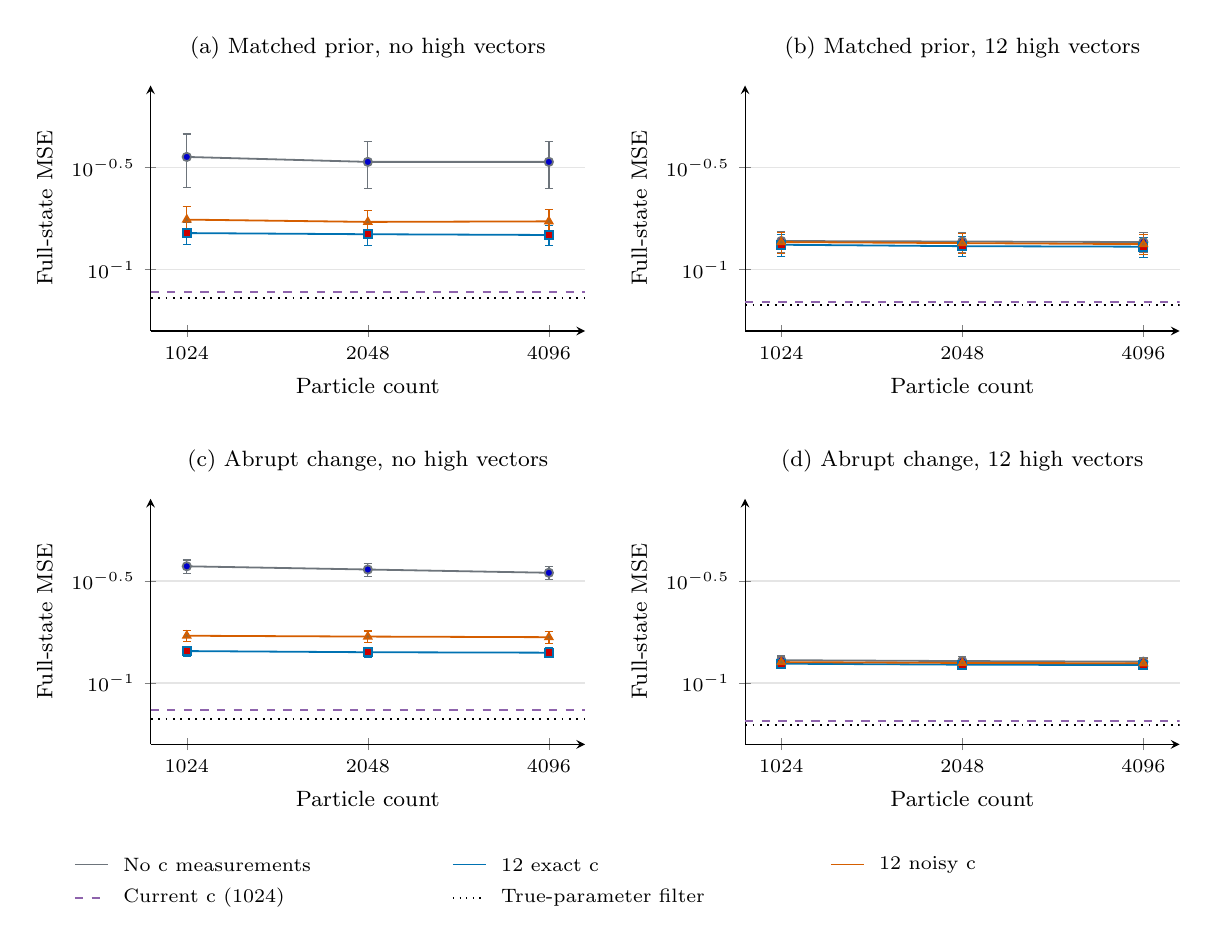
\begin{tikzpicture}
\begin{axis}[at={(0.0cm,5.75cm)},anchor=outer south west,width=7.1cm,height=4.7cm,font=\fontsize{8}{9.5}\selectfont,tick label style={font=\fontsize{7.5}{9}\selectfont},title style={align=left,font=\fontsize{8.5}{10}\selectfont},title={(a) Matched prior, no high vectors},axis x line=bottom,axis y line=left,ymajorgrids=true,grid style={gray!20},legend style={font=\fontsize{7}{8}\selectfont,draw=none,fill=none},ymode=log,ymin=.05,ymax=.8,xmin=-.2,xmax=2.2,xtick={0,1,2},xticklabels={1024,2048,4096},xlabel={Particle count},ylabel={Full-state MSE}]
\addplot+[color={rgb,255:red,109;green,116;blue,123},mark=*,mark size=1.5pt,line width=.65pt,solid,error bars/.cd,y dir=both,y explicit,error bar style={line width=.45pt}] coordinates {(0,0.356783481059) += (0,0.105405838101) -= (0,0.105405838101) (1,0.337384463503) += (0,0.0868503057975) -= (0,0.0868503057975) (2,0.337423142897) += (0,0.0885949945282) -= (0,0.0885949945282)};
\addplot+[color={rgb,255:red,0;green,114;blue,178},mark=square*,mark size=1.5pt,line width=.65pt,solid,error bars/.cd,y dir=both,y explicit,error bar style={line width=.45pt}] coordinates {(0,0.151000146697) += (0,0.0189203427679) -= (0,0.0189203427679) (1,0.149053395828) += (0,0.0179803730813) -= (0,0.0179803730813) (2,0.147803432124) += (0,0.0170648740099) -= (0,0.0170648740099)};
\addplot+[color={rgb,255:red,213;green,94;blue,0},mark=triangle*,mark size=1.5pt,line width=.65pt,solid,error bars/.cd,y dir=both,y explicit,error bar style={line width=.45pt}] coordinates {(0,0.175805319198) += (0,0.027101029198) -= (0,0.027101029198) (1,0.171321619817) += (0,0.0234660784047) -= (0,0.0234660784047) (2,0.172379513632) += (0,0.0238266999098) -= (0,0.0238266999098)};
\addplot[color={rgb,255:red,142;green,99;blue,172},dashed,no marks,forget plot,line width=.7pt] coordinates {(-0.2,0.07753744222986775) (2.2,0.07753744222986775)};
\addplot[color={rgb,255:red,0;green,0;blue,0},dotted,no marks,forget plot,line width=.7pt] coordinates {(-0.2,0.07273908832759599) (2.2,0.07273908832759599)};
\end{axis}
\begin{axis}[at={(7.55cm,5.75cm)},anchor=outer south west,width=7.1cm,height=4.7cm,font=\fontsize{8}{9.5}\selectfont,tick label style={font=\fontsize{7.5}{9}\selectfont},title style={align=left,font=\fontsize{8.5}{10}\selectfont},title={(b) Matched prior, 12 high vectors},axis x line=bottom,axis y line=left,ymajorgrids=true,grid style={gray!20},legend style={font=\fontsize{7}{8}\selectfont,draw=none,fill=none},ymode=log,ymin=.05,ymax=.8,xmin=-.2,xmax=2.2,xtick={0,1,2},xticklabels={1024,2048,4096},xlabel={Particle count},ylabel={Full-state MSE}]
\addplot+[color={rgb,255:red,109;green,116;blue,123},mark=*,mark size=1.5pt,line width=.65pt,solid,error bars/.cd,y dir=both,y explicit,error bar style={line width=.45pt}] coordinates {(0,0.138031807755) += (0,0.0162590579205) -= (0,0.0162590579205) (1,0.137299459735) += (0,0.0154343436317) -= (0,0.0154343436317) (2,0.136502600606) += (0,0.014945403974) -= (0,0.014945403974)};
\addplot+[color={rgb,255:red,0;green,114;blue,178},mark=square*,mark size=1.5pt,line width=.65pt,solid,error bars/.cd,y dir=both,y explicit,error bar style={line width=.45pt}] coordinates {(0,0.13235151917) += (0,0.0159547487753) -= (0,0.0159547487753) (1,0.130238220252) += (0,0.0145604209382) -= (0,0.0145604209382) (2,0.129503591012) += (0,0.0144786308565) -= (0,0.0144786308565)};
\addplot+[color={rgb,255:red,213;green,94;blue,0},mark=triangle*,mark size=1.5pt,line width=.65pt,solid,error bars/.cd,y dir=both,y explicit,error bar style={line width=.45pt}] coordinates {(0,0.136405591851) += (0,0.016096766709) -= (0,0.016096766709) (1,0.134836088472) += (0,0.0153656750135) -= (0,0.0153656750135) (2,0.1332810785) += (0,0.0146437295056) -= (0,0.0146437295056)};
\addplot[color={rgb,255:red,142;green,99;blue,172},dashed,no marks,forget plot,line width=.7pt] coordinates {(-0.2,0.06959728463581043) (2.2,0.06959728463581043)};
\addplot[color={rgb,255:red,0;green,0;blue,0},dotted,no marks,forget plot,line width=.7pt] coordinates {(-0.2,0.06685826411633457) (2.2,0.06685826411633457)};
\end{axis}
\begin{axis}[at={(0.0cm,0.5cm)},anchor=outer south west,width=7.1cm,height=4.7cm,font=\fontsize{8}{9.5}\selectfont,tick label style={font=\fontsize{7.5}{9}\selectfont},title style={align=left,font=\fontsize{8.5}{10}\selectfont},title={(c) Abrupt change, no high vectors},axis x line=bottom,axis y line=left,ymajorgrids=true,grid style={gray!20},legend style={font=\fontsize{7}{8}\selectfont,draw=none,fill=none},ymode=log,ymin=.05,ymax=.8,xmin=-.2,xmax=2.2,xtick={0,1,2},xticklabels={1024,2048,4096},xlabel={Particle count},ylabel={Full-state MSE}]
\addplot+[color={rgb,255:red,109;green,116;blue,123},mark=*,mark size=1.5pt,line width=.65pt,solid,error bars/.cd,y dir=both,y explicit,error bar style={line width=.45pt}] coordinates {(0,0.373389115047) += (0,0.0276630167858) -= (0,0.0276630167858) (1,0.360077820803) += (0,0.0267498513844) -= (0,0.0267498513844) (2,0.347017132013) += (0,0.0263813574851) -= (0,0.0263813574851)};
\addplot+[color={rgb,255:red,0;green,114;blue,178},mark=square*,mark size=1.5pt,line width=.65pt,solid,error bars/.cd,y dir=both,y explicit,error bar style={line width=.45pt}] coordinates {(0,0.143352592111) += (0,0.00780689672326) -= (0,0.00780689672326) (1,0.141497163196) += (0,0.00794714485384) -= (0,0.00794714485384) (2,0.140783597821) += (0,0.00792161975653) -= (0,0.00792161975653)};
\addplot+[color={rgb,255:red,213;green,94;blue,0},mark=triangle*,mark size=1.5pt,line width=.65pt,solid,error bars/.cd,y dir=both,y explicit,error bar style={line width=.45pt}] coordinates {(0,0.17044165982) += (0,0.0106435149261) -= (0,0.0106435149261) (1,0.168857264332) += (0,0.0108559380336) -= (0,0.0108559380336) (2,0.167700105984) += (0,0.0108542881357) -= (0,0.0108542881357)};
\addplot[color={rgb,255:red,142;green,99;blue,172},dashed,no marks,forget plot,line width=.7pt] coordinates {(-0.2,0.07377495644632073) (2.2,0.07377495644632073)};
\addplot[color={rgb,255:red,0;green,0;blue,0},dotted,no marks,forget plot,line width=.7pt] coordinates {(-0.2,0.0668910768328071) (2.2,0.0668910768328071)};
\end{axis}
\begin{axis}[at={(7.55cm,0.5cm)},anchor=outer south west,width=7.1cm,height=4.7cm,font=\fontsize{8}{9.5}\selectfont,tick label style={font=\fontsize{7.5}{9}\selectfont},title style={align=left,font=\fontsize{8.5}{10}\selectfont},title={(d) Abrupt change, 12 high vectors},axis x line=bottom,axis y line=left,ymajorgrids=true,grid style={gray!20},legend style={font=\fontsize{7}{8}\selectfont,draw=none,fill=none},ymode=log,ymin=.05,ymax=.8,xmin=-.2,xmax=2.2,xtick={0,1,2},xticklabels={1024,2048,4096},xlabel={Particle count},ylabel={Full-state MSE}]
\addplot+[color={rgb,255:red,109;green,116;blue,123},mark=*,mark size=1.5pt,line width=.65pt,solid,error bars/.cd,y dir=both,y explicit,error bar style={line width=.45pt}] coordinates {(0,0.129309875029) += (0,0.00621233301664) -= (0,0.00621233301664) (1,0.12806825954) += (0,0.00633394307316) -= (0,0.00633394307316) (2,0.127192155298) += (0,0.00627279526811) -= (0,0.00627279526811)};
\addplot+[color={rgb,255:red,0;green,114;blue,178},mark=square*,mark size=1.5pt,line width=.65pt,solid,error bars/.cd,y dir=both,y explicit,error bar style={line width=.45pt}] coordinates {(0,0.124291873457) += (0,0.00638521632489) -= (0,0.00638521632489) (1,0.122922994664) += (0,0.00651484102614) -= (0,0.00651484102614) (2,0.122389347101) += (0,0.00651213933059) -= (0,0.00651213933059)};
\addplot+[color={rgb,255:red,213;green,94;blue,0},mark=triangle*,mark size=1.5pt,line width=.65pt,solid,error bars/.cd,y dir=both,y explicit,error bar style={line width=.45pt}] coordinates {(0,0.126551720198) += (0,0.00632797351919) -= (0,0.00632797351919) (1,0.125356615012) += (0,0.00642263603365) -= (0,0.00642263603365) (2,0.124863994112) += (0,0.0064820700428) -= (0,0.0064820700428)};
\addplot[color={rgb,255:red,142;green,99;blue,172},dashed,no marks,forget plot,line width=.7pt] coordinates {(-0.2,0.0652864148382444) (2.2,0.0652864148382444)};
\addplot[color={rgb,255:red,0;green,0;blue,0},dotted,no marks,forget plot,line width=.7pt] coordinates {(-0.2,0.06206152299021828) (2.2,0.06206152299021828)};
\end{axis}
\draw[color={rgb,255:red,109;green,116;blue,123},solid] (0.6,-0.12) -- (1.02,-0.12);
\node[anchor=west,font=\fontsize{7.5}{9}\selectfont] at (1.0899999999999999,-0.12) {No c measurements};
\draw[color={rgb,255:red,0;green,114;blue,178},solid] (5.3999999999999995,-0.12) -- (5.819999999999999,-0.12);
\node[anchor=west,font=\fontsize{7.5}{9}\selectfont] at (5.89,-0.12) {12 exact c};
\draw[color={rgb,255:red,213;green,94;blue,0},solid] (10.2,-0.12) -- (10.62,-0.12);
\node[anchor=west,font=\fontsize{7.5}{9}\selectfont] at (10.69,-0.12) {12 noisy c};
\draw[color={rgb,255:red,142;green,99;blue,172},dashed] (0.6,-0.54) -- (1.02,-0.54);
\node[anchor=west,font=\fontsize{7.5}{9}\selectfont] at (1.0899999999999999,-0.54) {Current c (1024)};
\draw[color={rgb,255:red,0;green,0;blue,0},dotted] (5.3999999999999995,-0.54) -- (5.819999999999999,-0.54);
\node[anchor=west,font=\fontsize{7.5}{9}\selectfont] at (5.89,-0.54) {True-parameter filter};
\end{tikzpicture}
\caption{Finite parameter information evaluated on the same 32 saved observable trajectories per generating mechanism, with four algorithm seeds averaged within each trajectory. Points and bars show stored mean MSE values and descriptive 95\% trajectory intervals at 1,024, 2,048, and 4,096 particles. All three particle curves infer both $a$ and $c$. Exact and noisy arms receive 12 scalar measurements of $c$ at 10,30,...,230 after the current main estimate; noisy measurements have independent Gaussian standard deviation 0.1. The scalar-measurement budget is additional to the high-state-vector budget stated in the panel title. The dashed reference receives the current exact $c$ before prediction at all 240 steps and uses 1,024 particles; it is not a same-information or same-computation comparator at every plotted count. The dotted true-parameter filter receives both current parameters. Both references use the same 32 paths, and the lines show their means. Logarithmic axes are shared. These reused paths are not new confirmations.}
\label{fig:dynamics-parameter-information}
\end{figure}

The reduction in state error did not establish numerical stability. None of the eight parameter-measurement conditions passed all predefined criteria assessing terminal-count MSE change, state-estimate change, parameter-estimate change, and algorithm-seed variation. Consequently, lower average error does not establish a numerically resolved continuous-parameter posterior.

The final control varied only the fitted transition prior, holding true states, parameters, observations, initialization, and random streams fixed. On abrupt-change paths, halving diffusion standard deviation increased MSE by 0.082265 without new high observations ($[0.025371,0.139158]$), but reduced MSE by 0.028873 with twelve periodic observations (difference interval $[-0.032078,-0.025669]$). On matched-prior paths with periodic observations, both halving and doubling diffusion increased MSE. Among the sixteen primary contrasts, six intervals were positive, two were negative, and eight crossed zero. None of the twenty prior--condition combinations passed all four numerical criteria. These comparisons establish the effect of the prior within the finite algorithm, but do not separate exact-posterior misspecification from approximation error.

\section{Reliability reference and verification scope}
\label{app:reliability}

\subsection{Reference-model specifications}

Simulation failure and the low-innovation acquisition trigger are evaluated separately. The original endpoint required three consecutive pointwise threshold violations, with a full-state threshold equal to twice the time-averaged baseline low-only theoretical MSE after dense initialization. A subsequent endpoint uses the maximum ten-step mean standardized state error over the 240-step follow-up. Full-state squared-error sums are divided by the theoretical covariance trace of a known-baseline filter after twenty dense initialization steps and low-only follow-up; hidden-coordinate error uses the corresponding hidden covariance sum. For each observability condition, 4,096 independent no-change, state-only, low-only development trajectories determine the cutoff, defined as the 3,893rd order statistic of their maximum-window values. The cutoff is then evaluated on separate trajectories under that reference. This procedure calibrates a marginal event for the specified no-change filter and observation policy; other algorithms and policies share the cutoff without inheriting a 5\% guarantee.

The EEG reliability reference uses 4,491 initial-training out-of-fold correctness records from three fitted teachers. The teachers are fitted on smaller subsets than the original deployed model. Correctness parameters are inferred separately for each participant and class. The correlated reference is a stationary binary first-order Markov chain within same-class subsequences, with a 100-point grid for correctness probability $p$ and ten nonnegative persistence values $r=0,0.1,\ldots,0.9$. Each parameter draw is held fixed across the diagnostic and follow-up portions of a repetition; chain states reset at session and segment boundaries. The four arms compare a fixed independent posterior-mean probability, an independent probability draw, a correlated-posterior probability draw forced to $r=0$, and that identical probability draw with persistence also drawn. Each participant and arm has 32,768 repetitions. This reference generates correctness sequences without generating drift.

\subsection{Full reliability-reference comparisons}
\label{sec:reliability}


The original simulation failure rule recorded 466 failures among 512 observable no-change trajectories, even with true parameters and periodic high observations. The event therefore indicated repeated error-threshold violations rather than parameter drift. Calibration of a separate maximum-window endpoint on independent no-change trajectories produced full-state exceedances of 20/512, 29/512, and 23/512 under unobservable, weak, and observable coupling. These rates are 3.91\%, 5.66\%, and 4.49\%, close to the intended marginal no-change reference. This endpoint uses the true states available in simulation, distinguishing it from an observable online alarm.

The final EEG reference similarly evaluated how the reliability calculation depends on its assumptions. Across the fixed group of all 62 participants, simulated confirmed-failure probability was 73.348\% with the independent posterior mean fixed, 69.762\% after drawing the independent correctness probability, 69.958\% with correlated-model probability draws forced to independence, and 70.104\% with the identical probability draws and sampled nonnegative persistence. Introducing independent correctness-parameter uncertainty changed the probability by $-3.587$ percentage points (95\% interval $[-6.372,-0.709]$). Introducing persistence while holding the probability draws identical changed it by $+0.145$ points ($[+0.078,+0.216]$).

The group of 29 initially task-eligible participants was fixed before simulation and was not reselected afterward. Their uncertainty contrast was $-2.497$ percentage points ($[-6.169,+1.225]$), and their persistence contrast was $+0.116$ ($[+0.043,+0.197]$). The probabilities average all repetitions within the fixed groups, without conditioning on whether a repetition passes the simulated diagnostic criterion. Because the out-of-fold teachers differ from the original deployed teacher, these values cannot be subtracted from the original empirical failures to estimate a drift contribution or an actual EEG false-alarm rate.

Figure~\ref{fig:dynamics-reliability-reference} shows the four reference arms and their two controlled contrasts separately, with all-participant groups and fixed eligible subgroups on separate rows.

\begin{figure}[p]
\centering
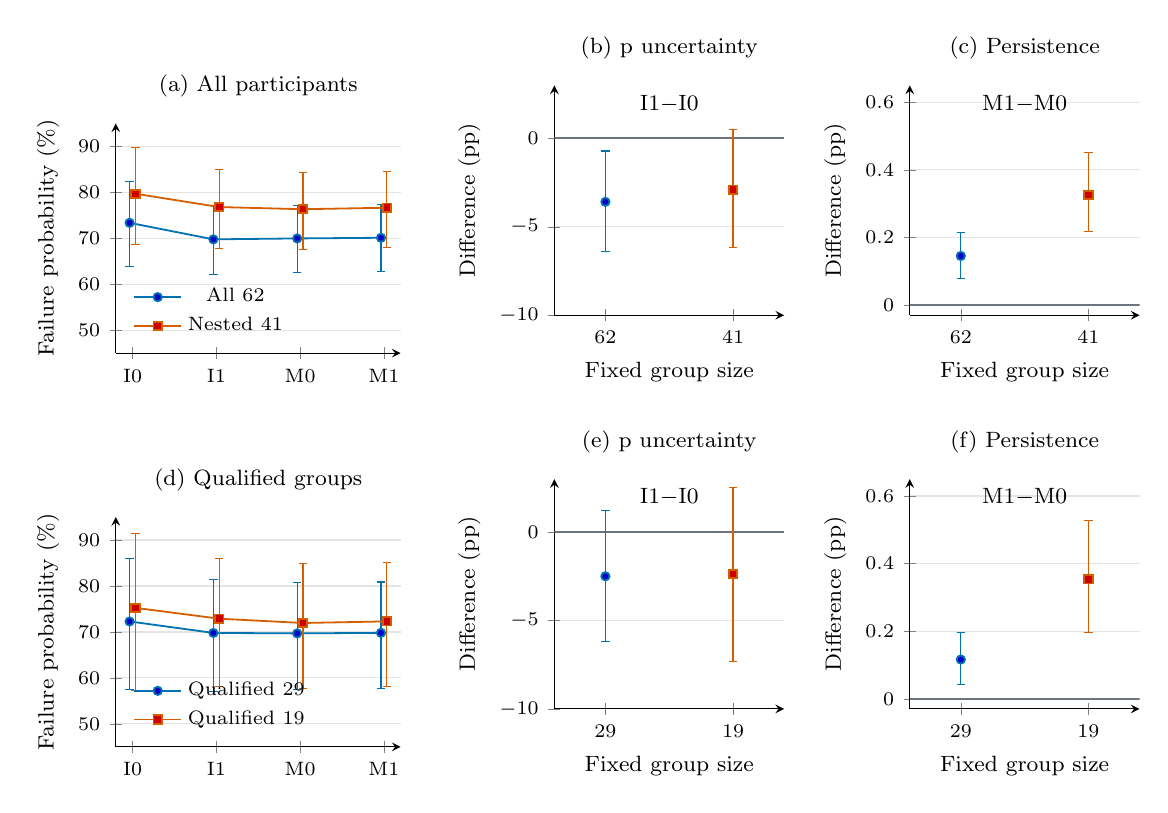
\begin{tikzpicture}
\begin{axis}[at={(0cm,5.0cm)},anchor=outer south west,width=5.2cm,height=4.5cm,font=\fontsize{8}{9.5}\selectfont,tick label style={font=\fontsize{7.5}{9}\selectfont},title style={align=left,font=\fontsize{8.5}{10}\selectfont},title={(a) All participants},axis x line=bottom,axis y line=left,ymajorgrids=true,grid style={gray!20},legend style={font=\fontsize{7}{8}\selectfont,draw=none,fill=none},xmin=-.2,xmax=3.2,ymin=45,ymax=95,ytick={50,60,70,80,90},xtick={0,1,2,3},xticklabels={I0,I1,M0,M1},ylabel={Failure probability (\%)},legend pos=south west]
\addplot+[color={rgb,255:red,0;green,114;blue,178},mark=*,mark size=1.5pt,line width=.65pt,solid,error bars/.cd,y dir=both,y explicit,error bar style={line width=.45pt}] coordinates {(-0.035,73.3484083606) += (0,8.92564712032) -= (0,9.40573292394) (0.965,69.7617069367) += (0,7.35917737407) -= (0,7.69910504741) (1.965,69.9582992061) += (0,7.23951278194) -= (0,7.45005822951) (2.965,70.1036022555) += (0,7.18811281266) -= (0,7.39289314516)};
\addlegendentry{All 62}
\addplot+[color={rgb,255:red,213;green,94;blue,0},mark=square*,mark size=1.5pt,line width=.65pt,solid,error bars/.cd,y dir=both,y explicit,error bar style={line width=.45pt}] coordinates {(0.035,79.6788657584) += (0,9.9948175942) -= (0,11.0875943812) (1.035,76.7872880145) += (0,8.12571083627) -= (0,8.94864710366) (2.035,76.3164241139) += (0,7.90821726729) -= (0,8.69049258348) (3.035,76.6422923018) += (0,7.82882876512) -= (0,8.58981248809)};
\addlegendentry{Nested 41}
\end{axis}
\begin{axis}[at={(5.35cm,5.0cm)},anchor=outer south west,width=4.5cm,height=4.5cm,font=\fontsize{8}{9.5}\selectfont,tick label style={font=\fontsize{7.5}{9}\selectfont},title style={align=left,font=\fontsize{8.5}{10}\selectfont},title={(b) p uncertainty},axis x line=bottom,axis y line=left,ymajorgrids=true,grid style={gray!20},legend style={font=\fontsize{7}{8}\selectfont,draw=none,fill=none},xmin=-.4,xmax=1.4,xtick={0,1},xticklabels={62,41},xlabel={Fixed group size},ylabel={Difference (pp)},ymin=-10,ymax=3,scaled y ticks=false,y tick label style={/pgf/number format/fixed,/pgf/number format/precision=2}]
\addplot[color={rgb,255:red,109;green,116;blue,123},solid,no marks,forget plot,line width=.7pt] coordinates {(-0.4,0) (1.4,0)};
\addplot+[color={rgb,255:red,0;green,114;blue,178},mark=*,mark size=1.5pt,line width=.65pt,only marks,error bars/.cd,y dir=both,y explicit,error bar style={line width=.45pt}] coordinates {(0,-3.58670142389) += (0,2.87743722239) -= (0,2.78496034684)};
\addplot+[color={rgb,255:red,213;green,94;blue,0},mark=square*,mark size=1.5pt,line width=.65pt,only marks,error bars/.cd,y dir=both,y explicit,error bar style={line width=.45pt}] coordinates {(1,-2.8915777439) += (0,3.41129582103) -= (0,3.28037541087)};
\node[font=\fontsize{8}{9}\selectfont] at (rel axis cs:.5,.92) {I1$-$I0};
\end{axis}
\begin{axis}[at={(10.0cm,5.0cm)},anchor=outer south west,width=4.5cm,height=4.5cm,font=\fontsize{8}{9.5}\selectfont,tick label style={font=\fontsize{7.5}{9}\selectfont},title style={align=left,font=\fontsize{8.5}{10}\selectfont},title={(c) Persistence},axis x line=bottom,axis y line=left,ymajorgrids=true,grid style={gray!20},legend style={font=\fontsize{7}{8}\selectfont,draw=none,fill=none},xmin=-.4,xmax=1.4,xtick={0,1},xticklabels={62,41},xlabel={Fixed group size},ylabel={Difference (pp)},ymin=-0.03,ymax=0.65,scaled y ticks=false,y tick label style={/pgf/number format/fixed,/pgf/number format/precision=2}]
\addplot[color={rgb,255:red,109;green,116;blue,123},solid,no marks,forget plot,line width=.7pt] coordinates {(-0.4,0) (1.4,0)};
\addplot+[color={rgb,255:red,0;green,114;blue,178},mark=*,mark size=1.5pt,line width=.65pt,only marks,error bars/.cd,y dir=both,y explicit,error bar style={line width=.45pt}] coordinates {(0,0.145303049395) += (0,0.0705866659841) -= (0,0.0670894499748)};
\addplot+[color={rgb,255:red,213;green,94;blue,0},mark=square*,mark size=1.5pt,line width=.65pt,only marks,error bars/.cd,y dir=both,y explicit,error bar style={line width=.45pt}] coordinates {(1,0.325868187881) += (0,0.125494235899) -= (0,0.108895650724)};
\node[font=\fontsize{8}{9}\selectfont] at (rel axis cs:.5,.92) {M1$-$M0};
\end{axis}
\begin{axis}[at={(0cm,0cm)},anchor=outer south west,width=5.2cm,height=4.5cm,font=\fontsize{8}{9.5}\selectfont,tick label style={font=\fontsize{7.5}{9}\selectfont},title style={align=left,font=\fontsize{8.5}{10}\selectfont},title={(d) Qualified groups},axis x line=bottom,axis y line=left,ymajorgrids=true,grid style={gray!20},legend style={font=\fontsize{7}{8}\selectfont,draw=none,fill=none},xmin=-.2,xmax=3.2,ymin=45,ymax=95,ytick={50,60,70,80,90},xtick={0,1,2,3},xticklabels={I0,I1,M0,M1},ylabel={Failure probability (\%)},legend pos=south west]
\addplot+[color={rgb,255:red,0;green,114;blue,178},mark=*,mark size=1.5pt,line width=.65pt,solid,error bars/.cd,y dir=both,y explicit,error bar style={line width=.45pt}] coordinates {(-0.035,72.284566945) += (0,13.6243649187) -= (0,14.789594453) (0.965,69.7878081223) += (0,11.5282755885) -= (0,12.6548346158) (1.965,69.6866791824) += (0,11.1261722959) -= (0,12.2646279171) (2.965,69.8028564453) += (0,11.0736741691) -= (0,12.2025772621)};
\addlegendentry{Qualified 29}
\addplot+[color={rgb,255:red,213;green,94;blue,0},mark=square*,mark size=1.5pt,line width=.65pt,solid,error bars/.cd,y dir=both,y explicit,error bar style={line width=.45pt}] coordinates {(0.035,75.243176912) += (0,16.1551144249) -= (0,18.0749471564) (1.035,72.8844893606) += (0,13.13958419) -= (0,14.7893042313) (2.035,71.946796618) += (0,12.9590566535) -= (0,14.3441210295) (3.035,72.2999974301) += (0,12.8553892437) -= (0,14.2397950825)};
\addlegendentry{Qualified 19}
\end{axis}
\begin{axis}[at={(5.35cm,0cm)},anchor=outer south west,width=4.5cm,height=4.5cm,font=\fontsize{8}{9.5}\selectfont,tick label style={font=\fontsize{7.5}{9}\selectfont},title style={align=left,font=\fontsize{8.5}{10}\selectfont},title={(e) p uncertainty},axis x line=bottom,axis y line=left,ymajorgrids=true,grid style={gray!20},legend style={font=\fontsize{7}{8}\selectfont,draw=none,fill=none},xmin=-.4,xmax=1.4,xtick={0,1},xticklabels={29,19},xlabel={Fixed group size},ylabel={Difference (pp)},ymin=-10,ymax=3,scaled y ticks=false,y tick label style={/pgf/number format/fixed,/pgf/number format/precision=2}]
\addplot[color={rgb,255:red,109;green,116;blue,123},solid,no marks,forget plot,line width=.7pt] coordinates {(-0.4,0) (1.4,0)};
\addplot+[color={rgb,255:red,0;green,114;blue,178},mark=*,mark size=1.5pt,line width=.65pt,only marks,error bars/.cd,y dir=both,y explicit,error bar style={line width=.45pt}] coordinates {(0,-2.49675882274) += (0,3.72220269565) -= (0,3.67200654129)};
\addplot+[color={rgb,255:red,213;green,94;blue,0},mark=square*,mark size=1.5pt,line width=.65pt,only marks,error bars/.cd,y dir=both,y explicit,error bar style={line width=.45pt}] coordinates {(1,-2.3586875514) += (0,4.90419488204) -= (0,4.96039139597)};
\node[font=\fontsize{8}{9}\selectfont] at (rel axis cs:.5,.92) {I1$-$I0};
\end{axis}
\begin{axis}[at={(10.0cm,0cm)},anchor=outer south west,width=4.5cm,height=4.5cm,font=\fontsize{8}{9.5}\selectfont,tick label style={font=\fontsize{7.5}{9}\selectfont},title style={align=left,font=\fontsize{8.5}{10}\selectfont},title={(f) Persistence},axis x line=bottom,axis y line=left,ymajorgrids=true,grid style={gray!20},legend style={font=\fontsize{7}{8}\selectfont,draw=none,fill=none},xmin=-.4,xmax=1.4,xtick={0,1},xticklabels={29,19},xlabel={Fixed group size},ylabel={Difference (pp)},ymin=-0.03,ymax=0.65,scaled y ticks=false,y tick label style={/pgf/number format/fixed,/pgf/number format/precision=2}]
\addplot[color={rgb,255:red,109;green,116;blue,123},solid,no marks,forget plot,line width=.7pt] coordinates {(-0.4,0) (1.4,0)};
\addplot+[color={rgb,255:red,0;green,114;blue,178},mark=*,mark size=1.5pt,line width=.65pt,only marks,error bars/.cd,y dir=both,y explicit,error bar style={line width=.45pt}] coordinates {(0,0.116177262931) += (0,0.0806111302869) -= (0,0.073347420528)};
\addplot+[color={rgb,255:red,213;green,94;blue,0},mark=square*,mark size=1.5pt,line width=.65pt,only marks,error bars/.cd,y dir=both,y explicit,error bar style={line width=.45pt}] coordinates {(1,0.353200812089) += (0,0.174925954718) -= (0,0.156767995734)};
\node[font=\fontsize{8}{9}\selectfont] at (rel axis cs:.5,.92) {M1$-$M0};
\end{axis}
\end{tikzpicture}
\caption{Correctness uncertainty and same-class persistence in the training-only EEG reliability reference. The rows separate all 62 participants and the nested 41 from the fixed initially task-qualified groups of 29 and 19. (a,d) I0 fixes the independent posterior-mean correctness probability; I1 draws it from the independent posterior; M0 uses a probability drawn from the Markov posterior but sets persistence to zero; M1 uses exactly the same probability draws and sampled persistence. (b,e) I1 minus I0 isolates the specified correctness-parameter uncertainty. (c,f) M1 minus M0 isolates the specified same-class persistence at identical probability draws. The two contrast columns use different scales. Points and bars show the stored means and conditional 95\% participant-bootstrap intervals (10,000 resamples; teachers and posteriors fixed), not Monte Carlo intervals or a full shared-training uncertainty analysis. Each arm uses 32,768 repetitions per participant; probabilities include every repetition in each fixed group, without reselecting participants according to simulated diagnostic success. Nested groups are not independent confirmations. These surrogate teachers do not calibrate the deployed teacher or estimate actual EEG drift.}
\label{fig:dynamics-reliability-reference}
\end{figure}

The maximum-window simulation cutoff is the value at rank 3,893 among 4,096 independent calibration values. Under a continuous exchangeable reference, its marginal exceedance probability is $(4097-3893)/4097\approx4.98\%$. Validation reports exceedance counts and binomial intervals by observability condition. The error statistic depends on known simulation state, whereas the acquisition trigger depends on observed innovation. Calibrating one therefore does not calibrate the other.

The original pointwise threshold is twice the mean theoretical baseline low-only variance per coordinate over follow-up after dense initialization. Three successive exceedances confirm failure, with onset and confirmation stored separately. For the calibrated endpoint, failure is recorded at the end of the first ten-step window that exceeds the cutoff; ten successive acceptable windows confirm recovery. The start of a window is not interpreted as an estimate of change onset.

The EEG correlated reference contains 124 participant--class units and 1,605 within-class transitions after segmentation. Transition counts range from 1 to 36, with median 12. The finite-grid calculation evaluates the likelihood of all segment starts and transitions. For state $b\in\{0,1\}$ and correctness probability $p$, the stationary persistence parameterization uses
\begin{equation}
 P(B_{t+1}=1\mid B_t=1)=p+r(1-p),\qquad
 P(B_{t+1}=1\mid B_t=0)=p(1-r).
\end{equation}
The analysis examines only nonnegative persistence values. The model addresses order in same-class subsequences, not waveform autocorrelation, physical-time dependence, or cross-day persistence. The finite-grid posterior is exact for the chosen grid and likelihood, but not for all continuous or nonstationary alternatives.

Probability locations are $p_k=(k+0.5)/100$, $k=0,\ldots,99$, with prior mass proportional to $[p_k(1-p_k)]^{-1/2}$. Persistence has uniform prior mass over its ten grid values, independently of correctness probability. Training segments break at participant, session, teacher fold, recording run, or task changes and at gaps in original trial ordinal. Evaluation uses the same segmentation rules except for teacher-fold boundaries. Separate same-class subsequences are formed within each intact segment, with opposite-class trials allowed between adjacent members of a class subsequence. Segment starts are independent Bernoulli draws at the sampled class probability; parameters persist across sessions, but chain state does not.

The three out-of-fold teachers yield 1,511, 1,501, and 1,479 evaluated rows, with base fitting subsets of 2,358, 2,366, and 2,382 rows after excluding the outer fold and its internal holdout block. Parameter and event-innovation streams use PCG64DXSM seeds 2026101101 and 2026101102; participant resampling uses seed 2026101111, using the participant, class, arm, and repetition indexing specified in the protocol.

Table~\ref{tab:reliability} reports results for all four fixed population definitions. Within each group, probabilities average all repetitions, including those that fail the simulated diagnostic eligibility criterion. Teachers and posteriors remain fixed during participant resampling. The historical independent reference for the original deployed teacher had failure probabilities 14.469\% in the initially eligible 29 and 22.415\% in the eligible nested 19. Those teacher-specific references obtain correctness estimates from a different source than the out-of-fold reference below; their difference therefore does not estimate correlation or drift.

\begin{table}[h]
\centering\small
\caption{Changes in simulated confirmed-failure probability, in percentage points. The uncertainty contrast subtracts the result with the independent posterior mean fixed from the result with an independent probability draw. The persistence contrast uses identical probability draws in both arms. Intervals are conditional 95\% participant-bootstrap intervals.}
\label{tab:reliability}
\begin{tabular}{@{}lrr@{}}
\toprule
Fixed participant group & Uncertainty contrast & Persistence contrast\\
\midrule
All 62 & $-3.587\;[-6.372,-0.709]$ & $+0.145\;[+0.078,+0.216]$\\
Initial task-eligible 29 & $-2.497\;[-6.169,+1.225]$ & $+0.116\;[+0.043,+0.197]$\\
Nested 41 & $-2.892\;[-6.172,+0.520]$ & $+0.326\;[+0.217,+0.451]$\\
Initial task-eligible nested 19 & $-2.359\;[-7.319,+2.546]$ & $+0.353\;[+0.196,+0.528]$\\
\bottomrule
\end{tabular}
\end{table}

Independent verification reconstructs available-information identities, split exclusions, prediction order, parameter chains, and metrics within the scopes specified in the archive. The final dynamics prior study contains 5,120 method paths. A separate CPU implementation fully replays 1,280 paths from the fixed trajectory subset, while stored-metric checks cover all 5,120 paths. Baseline arrays are also checked against previously sealed files. Reliability verification recomputes the finite-grid likelihoods, controlled draw identities, event logic, and aggregated quantities. These checks establish consistency between the protocol and saved artifacts within the stated scopes. They provide neither a second raw EEG collection nor a proof that finite inference equals an exact continuous posterior.


Reliability adds a decision rule to the prediction problem. The original repeated-error event occurred frequently even in a no-change simulation; the calibrated maximum-window event addresses a specified no-change reference. Failure probabilities in the EEG correctness reference likewise changed with parameter uncertainty or same-class persistence. Its out-of-fold teachers differ from the deployed teacher, so these reference effects cannot be subtracted from empirical failures to estimate biological drift or an actual EEG alarm rate. A reliability statement must identify its event, reference population, model assumptions, and follow-up unit.

\begin{thebibliography}{99}

\bibitem{vidaurre2011}
C. Vidaurre, M. Kawanabe, P. von B{\"u}nau, B. Blankertz, and K. R. M{\"u}ller.
Toward Unsupervised Adaptation of LDA for Brain--Computer Interfaces.
\emph{IEEE Transactions on Biomedical Engineering}, 58(3):587--597, 2011.
\href{https://doi.org/10.1109/TBME.2010.2093133}{doi:10.1109/TBME.2010.2093133}.

\bibitem{lotte2018}
F. Lotte, L. Bougrain, A. Cichocki, M. Clerc, M. Congedo, A. Rakotomamonjy, and F. Yger.
A review of classification algorithms for EEG-based brain--computer interfaces: a 10 year update.
\emph{Journal of Neural Engineering}, 15(3):031005, 2018.
\href{https://doi.org/10.1088/1741-2552/aab2f2}{doi:10.1088/1741-2552/aab2f2}.

\bibitem{jayaram2016}
V. Jayaram, M. Alamgir, Y. Altun, B. Sch{\"o}lkopf, and M. Grosse-Wentrup.
Transfer Learning in Brain-Computer Interfaces.
\emph{IEEE Computational Intelligence Magazine}, 11(1):20--31, 2016.
\href{https://doi.org/10.1109/MCI.2015.2501545}{doi:10.1109/MCI.2015.2501545}.

\bibitem{barachant2012}
A. Barachant, S. Bonnet, M. Congedo, and C. Jutten.
Multiclass Brain--Computer Interface Classification by Riemannian Geometry.
\emph{IEEE Transactions on Biomedical Engineering}, 59(4):920--928, 2012.
\href{https://doi.org/10.1109/TBME.2011.2172210}{doi:10.1109/TBME.2011.2172210}.

\bibitem{zanini2018}
P. Zanini, M. Congedo, C. Jutten, S. Said, and Y. Berthoumieu.
Transfer Learning: A Riemannian Geometry Framework With Applications to Brain--Computer Interfaces.
\emph{IEEE Transactions on Biomedical Engineering}, 65(5):1107--1116, 2018.
\href{https://doi.org/10.1109/TBME.2017.2742541}{doi:10.1109/TBME.2017.2742541}.

\bibitem{rodrigues2019}
P. L. C. Rodrigues, C. Jutten, and M. Congedo.
Riemannian Procrustes Analysis: Transfer Learning for Brain--Computer Interfaces.
\emph{IEEE Transactions on Biomedical Engineering}, 66(8):2390--2401, 2019.
\href{https://doi.org/10.1109/TBME.2018.2889705}{doi:10.1109/TBME.2018.2889705}.

\bibitem{vapnik2009}
V. Vapnik and A. Vashist.
A new learning paradigm: Learning using privileged information.
\emph{Neural Networks}, 22(5--6):544--557, 2009.
\href{https://doi.org/10.1016/j.neunet.2009.06.042}{doi:10.1016/j.neunet.2009.06.042}.

\bibitem{lopezpaz2016}
D. Lopez-Paz, L. Bottou, B. Sch\"olkopf, and V. Vapnik.
Unifying distillation and privileged information.
In \emph{Proceedings of the International Conference on Learning Representations}, 2016.
\href{https://www.iclr.cc/archive/www/2016.html}{Published conference record}.

\bibitem{kirkpatrick2017}
J. Kirkpatrick et al.
Overcoming catastrophic forgetting in neural networks.
\emph{Proceedings of the National Academy of Sciences}, 114(13):3521--3526, 2017.
\href{https://doi.org/10.1073/pnas.1611835114}{doi:10.1073/pnas.1611835114}.

\bibitem{li2018}
Z. Li and D. Hoiem.
Learning without Forgetting.
\emph{IEEE Transactions on Pattern Analysis and Machine Intelligence}, 40(12):2935--2947, 2018.
\href{https://doi.org/10.1109/TPAMI.2017.2773081}{doi:10.1109/TPAMI.2017.2773081}.

\bibitem{lopezpaz2017}
D. Lopez-Paz and M. Ranzato.
Gradient Episodic Memory for Continual Learning.
\emph{Advances in Neural Information Processing Systems}, 30, 2017.
\href{https://proceedings.nips.cc/paper_files/paper/2017/hash/f87522788a2be2d171666752f97ddebb-Abstract.html}{Published proceedings}.

\bibitem{jayaram2018}
V. Jayaram and A. Barachant.
MOABB: trustworthy algorithm benchmarking for BCIs.
\emph{Journal of Neural Engineering}, 15(6):066011, 2018.
\href{https://doi.org/10.1088/1741-2552/aadea0}{doi:10.1088/1741-2552/aadea0}.

\bibitem{mikkelsen2017}
K. B. Mikkelsen, P. Kidmose, and L. K. Hansen.
On the Keyhole Hypothesis: High Mutual Information between Ear and Scalp EEG.
\emph{Frontiers in Human Neuroscience}, 11:341, 2017.
\href{https://doi.org/10.3389/fnhum.2017.00341}{doi:10.3389/fnhum.2017.00341}.

\bibitem{fan2023}
C. Fan, N. Hahn, F. Kamdar, D. Avansino, G. H. Wilson, L. Hochberg, K. V. Shenoy, J. M. Henderson, and F. R. Willett.
Plug-and-Play Stability for Intracortical Brain-Computer Interfaces: A One-Year Demonstration of Seamless Brain-to-Text Communication.
\emph{Advances in Neural Information Processing Systems}, 36:42258--42270, 2023.
\href{https://proceedings.neurips.cc/paper_files/paper/2023/hash/83a14a36de4502bac5b580db36e81858-Abstract-Conference.html}{Published proceedings}. \href{https://doi.org/10.52202/075280-1831}{doi:10.52202/075280-1831}.

\bibitem{karpowicz2025}
B. M. Karpowicz et al.
Stabilizing brain-computer interfaces through alignment of latent dynamics.
\emph{Nature Communications}, 16:4662, 2025.
\href{https://doi.org/10.1038/s41467-025-59652-y}{doi:10.1038/s41467-025-59652-y}.

\bibitem{ramakrishnan2016}
A. G. Ramakrishnan and J. V. Satyanarayana.
Reconstruction of EEG from limited channel acquisition using estimated signal correlation.
\emph{Biomedical Signal Processing and Control}, 27:164--173, 2016.
\href{https://doi.org/10.1016/j.bspc.2016.02.004}{doi:10.1016/j.bspc.2016.02.004}.

\bibitem{duan2024}
T. Duan, Z. Wang, F. Li, G. Doretto, D. A. Adjeroh, Y. Yin, and C. Tao.
Online continual decoding of streaming EEG signal with a balanced and informative memory buffer.
\emph{Neural Networks}, 176:106338, 2024.
\href{https://doi.org/10.1016/j.neunet.2024.106338}{doi:10.1016/j.neunet.2024.106338}.

\bibitem{stieger2021}
J. R. Stieger, S. A. Engel, and B. He.
Continuous sensorimotor rhythm based brain computer interface learning in a large population.
\emph{Scientific Data}, 8:98, 2021.
\href{https://doi.org/10.1038/s41597-021-00883-1}{doi:10.1038/s41597-021-00883-1}.

\bibitem{lee2019}
M.-H. Lee, O.-Y. Kwon, Y.-J. Kim, H.-K. Kim, Y.-E. Lee, J. Williamson, S. Fazli, and S.-W. Lee.
EEG dataset and OpenBMI toolbox for three BCI paradigms: an investigation into BCI illiteracy.
\emph{GigaScience}, 8(5):giz002, 2019.
\href{https://doi.org/10.1093/gigascience/giz002}{doi:10.1093/gigascience/giz002}.

\bibitem{yang2025}
B. Yang, F. Rong, Y. Xie, D. Li, J. Zhang, F. Li, G. Shi, and X. Gao.
A multi-day and high-quality EEG dataset for motor imagery brain-computer interface.
\emph{Scientific Data}, 12:488, 2025.
\href{https://doi.org/10.1038/s41597-025-04826-y}{doi:10.1038/s41597-025-04826-y}.

\bibitem{farabbi2020}
A. Farabbi, F. Ghiringhelli, L. Mainardi, J. M. Sanches, P. Moreno, J. Santos-Victor, P. Figueiredo, and A. Vourvopoulos.
Motor-Imagery EEG Dataset During Robot-Arm Control. Version 1, Zenodo, 2020.
\href{https://doi.org/10.5281/zenodo.5882500}{doi:10.5281/zenodo.5882500}.

\bibitem{delong1988}
E. R. DeLong, D. M. DeLong and D. L. Clarke-Pearson.
Comparing the Areas under Two or More Correlated Receiver Operating Characteristic Curves: A Nonparametric Approach.
\emph{Biometrics}, 44(3):837--845, 1988.
\href{https://doi.org/10.2307/2531595}{doi:10.2307/2531595}.

\bibitem{reve2025}
Y. El Ouahidi, J. Lys, P. Th\"olke, N. Farrugia, B. Pasdeloup, V. Gripon, K. Jerbi, and G. Lioi.
REVE: A Foundation Model for EEG---Adapting to Any Setup with Large-Scale Pretraining on 25,000 Subjects.
\emph{Advances in Neural Information Processing Systems}, 38, 2025.
\href{https://proceedings.neurips.cc/paper_files/paper/2025/hash/20a917f77773ac0fa8bea2bdd6606b66-Abstract-Conference.html}{Published proceedings}.

\bibitem{blankertz2011}
B. Blankertz, S. Lemm, M. Treder, S. Haufe, and K.-R. M{\"u}ller.
Single-trial analysis and classification of ERP components --- A tutorial.
\emph{NeuroImage}, 56(2):814--825, 2011.
\href{https://doi.org/10.1016/j.neuroimage.2010.06.048}{doi:10.1016/j.neuroimage.2010.06.048}.

\bibitem{chen2010}
Y. Chen, A. Wiesel, Y. C. Eldar and A. O. Hero.
Shrinkage Algorithms for MMSE Covariance Estimation.
\emph{IEEE Transactions on Signal Processing}, 58(10):5016--5029, 2010.
\href{https://doi.org/10.1109/TSP.2010.2053029}{doi:10.1109/TSP.2010.2053029}.

\bibitem{efron1979}
B. Efron.
Bootstrap Methods: Another Look at the Jackknife.
\emph{The Annals of Statistics}, 7(1):1--26, 1979.
\href{https://doi.org/10.1214/aos/1176344552}{doi:10.1214/aos/1176344552}.

\bibitem{sannelli2019}
C. Sannelli, C. Vidaurre, K.-R. M{\"u}ller, and B. Blankertz.
A large scale screening study with a SMR-based BCI: Categorization of BCI users and differences in their SMR activity.
\emph{PLOS ONE}, 14(1):e0207351, 2019.
\href{https://doi.org/10.1371/journal.pone.0207351}{doi:10.1371/journal.pone.0207351}.

\bibitem{chaudhry2018}
A. Chaudhry, P. K. Dokania, T. Ajanthan, and P. H. S. Torr.
Riemannian Walk for Incremental Learning: Understanding Forgetting and Intransigence.
In \emph{Computer Vision--ECCV 2018}, Lecture Notes in Computer Science, vol. 11215, pp. 556--572, 2018.
\href{https://doi.org/10.1007/978-3-030-01252-6_33}{doi:10.1007/978-3-030-01252-6\_33}.

\bibitem{delange2022}
M. De Lange, R. Aljundi, M. Masana, S. Parisot, X. Jia, A. Leonardis, G. Slabaugh, and T. Tuytelaars.
A Continual Learning Survey: Defying Forgetting in Classification Tasks.
\emph{IEEE Transactions on Pattern Analysis and Machine Intelligence}, 44(7):3366--3385, 2022.
\href{https://doi.org/10.1109/TPAMI.2021.3057446}{doi:10.1109/TPAMI.2021.3057446}.

\bibitem{rebuffi2017}
S.-A. Rebuffi, A. Kolesnikov, G. Sperl, and C. H. Lampert.
iCaRL: Incremental Classifier and Representation Learning.
In \emph{2017 IEEE Conference on Computer Vision and Pattern Recognition}, pp. 5533--5542, 2017.
\href{https://doi.org/10.1109/CVPR.2017.587}{doi:10.1109/CVPR.2017.587}.

\bibitem{hermann1977}
R. Hermann and A. J. Krener.
Nonlinear Controllability and Observability.
\emph{IEEE Transactions on Automatic Control}, 22(5):728--740, 1977.
\href{https://doi.org/10.1109/TAC.1977.1101601}{doi:10.1109/TAC.1977.1101601}.

\bibitem{sinopoli2004}
B. Sinopoli, L. Schenato, M. Franceschetti, K. Poolla, M. I. Jordan, and S. S. Sastry.
Kalman Filtering With Intermittent Observations.
\emph{IEEE Transactions on Automatic Control}, 49(9):1453--1464, 2004.
\href{https://doi.org/10.1109/TAC.2004.834121}{doi:10.1109/TAC.2004.834121}.

\bibitem{sandberg2008}
H. Sandberg, M. Rabi, M. Skoglund, and K. H. Johansson.
Estimation over Heterogeneous Sensor Networks.
In \emph{Proceedings of the 47th IEEE Conference on Decision and Control}, pp. 4898--4903, 2008.
\href{https://doi.org/10.1109/CDC.2008.4739474}{doi:10.1109/CDC.2008.4739474}.

\bibitem{ahdab2025}
M. Al Ahdab, J. Leth, and Z.-H. Tan.
Optimal Sensor Scheduling and Selection for Continuous-Discrete Kalman Filtering with Auxiliary Dynamics.
In \emph{Proceedings of the 42nd International Conference on Machine Learning}, PMLR 267:703--729, 2025.
\href{https://proceedings.mlr.press/v267/ahdab25a.html}{Published proceedings}.

\bibitem{yao2024}
D. Yao, D. Xu, S. Lachapelle, S. Magliacane, P. Taslakian, G. Martius, J. von K\"ugelgen, and F. Locatello.
Multi-View Causal Representation Learning with Partial Observability.
In \emph{Proceedings of the International Conference on Learning Representations}, 2024.
\href{https://proceedings.iclr.cc/paper_files/paper/2024/hash/956e5427549a82a7472e02adc88360e9-Abstract-Conference.html}{Published proceedings}.

\bibitem{kalman1960}
R. E. Kalman.
A New Approach to Linear Filtering and Prediction Problems.
\emph{Journal of Basic Engineering}, 82(1):35--45, 1960.
\href{https://doi.org/10.1115/1.3662552}{doi:10.1115/1.3662552}.

\bibitem{doucet2000}
A. Doucet, S. Godsill and C. Andrieu.
On sequential Monte Carlo sampling methods for Bayesian filtering.
\emph{Statistics and Computing}, 10(3):197--208, 2000.
\href{https://doi.org/10.1023/A:1008935410038}{doi:10.1023/A:1008935410038}.

\end{thebibliography}

\end{document}
